%!TEX TS-program = xelatex

%!TEX root = ../Thesis.tex

% This information is used in titlepage, colophon, preface and hyperref setup (pdf metainfo), and other options.

%\def\thesistypeabbr{B.Eng.}
%\def\thesistype    {Bachelor of Engineering}
%\def\thesistypeabbr{B.Sc.Eng.}
%\def\thesistype    {Bachelor of Science in Engineering}
\def\thesistypeabbr{Ph.D.}
\def\thesistype    {Doctor of Philosophy}

\def\thesisauthor  {Jesper S{\"o}ren Dramsch}
\def\thesistitle   {Machine Learning in\\ 4D Seismic Data Analysis}
\def\thesissubtitle{Deep Neural Networks in Geophysics}
\def\thesislocation{Kongens Lyngby}

\def\papersize    {a4paper} % Final papersize (b5paper/a4paper), recommended papersize for DTU Compute is b5paper
\def\showtrims    {false} % Print on larger paper than \papersize and show trim marks (true/false)?

\def\showtodos    {false}  % Show todos (true/false)?
\def\confidential {false} % Confidential thesis (true/false)?


%!TEX root = ../Thesis.tex
\RequirePackage[l2tabu,orthodox]{nag} % Old habits die hard

\newcommand{\papersizeswitch}[3]{\ifnum\strcmp{\papersize}{#1}=0#2\else#3\fi}
\papersizeswitch{b5paper}{\def\classfontsize{10pt}}{\def\classfontsize{12pt}}

\documentclass[\classfontsize,\papersize,twoside,showtrims,extrafontsizes]{memoir}
\RequireXeTeX

\showtrimsoff
\papersizeswitch{b5paper}{
    % Stock and paper layout
    \pagebv
    \setlrmarginsandblock{26mm}{20mm}{*}
    \setulmarginsandblock{35mm}{30mm}{*}
    \setheadfoot{8mm}{10mm}
    \setlength{\headsep}{7mm}
    \setlength{\marginparwidth}{18mm}
    \setlength{\marginparsep}{2mm}
}{
    \papersizeswitch{a4paper}{
        \pageaiv
        \setlength{\trimtop}{0pt}
        \setlength{\trimedge}{\stockwidth}
        \addtolength{\trimedge}{-\paperwidth}
        \settypeblocksize{634pt}{448.13pt}{*}
        \setulmargins{4cm}{*}{*}
        \setlrmargins{*}{*}{0.66}
        \setmarginnotes{17pt}{51pt}{\onelineskip}
        \setheadfoot{\onelineskip}{2\onelineskip}
        \setheaderspaces{*}{2\onelineskip}{*}
    }{
    }
}
\ifnum\strcmp{\showtrims}{true}=0
    % For printing B5 on A4 with trimmarks
    \showtrimson
    \papersizeswitch{b5paper}{\stockaiv}{\stockaiii}
    \setlength{\trimtop}{\stockheight}
    \addtolength{\trimtop}{-\paperheight}
    \setlength{\trimtop}{0.5\trimtop}
    \setlength{\trimedge}{\stockwidth}
    \addtolength{\trimedge}{-\paperwidth}
    \setlength{\trimedge}{0.5\trimedge}
    
    % bigger todos if trim marks
    \setmarginnotes{10pt}{95pt}{\onelineskip}

    \trimLmarks
    
    % put jobname in left top trim mark
    \renewcommand*{\tmarktl}{%
      \begin{picture}(0,0)
        \unitlength 1mm
        \thinlines
        \put(-2,0){\line(-1,0){18}}
        \put(0,2){\line(0,1){18}}
        \put(3,15){\normalfont\ttfamily\fontsize{8bp}{10bp}\selectfont\jobname\ \
          \today\ \ 
          \printtime\ \ 
          Page \thepage}
      \end{picture}}

    % Remove middle trim marks for cleaner layout
    \renewcommand*{\tmarktm}{}
    \renewcommand*{\tmarkml}{}
    \renewcommand*{\tmarkmr}{}
    \renewcommand*{\tmarkbm}{}
\fi

\checkandfixthelayout                 % Check if errors in paper format!
\sideparmargin{outer}                 % Put sidemargins in outer position (why the fuck is this option not default by the class?)

% Large environments
\usepackage{microtype}
\usepackage{mathtools}
\usepackage{listings}                 % Source code printer for LaTeX
\usepackage{tikz}

% Links
\usepackage[hyphens]{url}             % Allow hyphens in URL's
\usepackage[unicode=false,psdextra]{hyperref}                 % References package

% Graphics and colors
\usepackage{graphicx}                 % Including graphics and using colours
\usepackage{xcolor}                   % Defined more color names
\usepackage{eso-pic}                  % Watermark and other bag
\usepackage{svg}
\usepackage{preamble/dtucolors}
\graphicspath{{graphics/}}

% Language
\usepackage{polyglossia}    % multilingual typesetting and appropriate hyphenation
\setdefaultlanguage{english}
\usepackage{csquotes}       % language sensitive quotation facilities


% Bibliography (references)
\usepackage[backend=biber,
            style=authoryear,
            %backref=true,
            dashed=false,
            %abbreviate=false,
            %dateabbrev=false,
            natbib=true,
            uniquename=false,
            giveninits=true,
            %citetracker=true,
            %useprefix=false,
            %uniquelist=false,
            minnames=1,
            alldates=long,
            sorting=nyt,
            maxnames=2,
            maxbibnames=99]{biblatex}

\preto\fullcite{\AtNextCite{\defcounter{maxnames}{99}}}


% Floating objets, captions and references
\usepackage{flafter}  % floats is positioned after or where it is defined! 
%\setfloatlocations{figure}{bhtp}   % Set floats for all figures
%\setfloatlocations{table}{bhtp}    % Set floats for all tables
%\setFloatBlockFor{section}         % Typeset floats before each section
\usepackage[noabbrev,nameinlink,capitalise]{cleveref} % Clever references. Options: "fig. !1!" --> "!Figure 1!"
\hangcaption
\captionnamefont{\bfseries}
\subcaptionlabelfont{\bfseries}
\newsubfloat{figure}
\newsubfloat{table}
%\letcountercounter{figure}{table}         % Consecutive table and figure numbering
%\letcountercounter{lstlisting}{table}     % Consecutive table and listings numbering
\captiontitlefinal{.}
% strip things from equation references, making them "(1)" instead of "Equation~1"
% from http://tex.stackexchange.com/questions/122174/how-to-strip-eq-from-cleveref
\crefformat{equation}{(#2#1#3)}
\crefrangeformat{equation}{(#3#1#4) to~(#5#2#6)}
\crefmultiformat{equation}{(#2#1#3)}%
{ and~(#2#1#3)}{, (#2#1#3)}{ and~(#2#1#3)}

% Table of contents (TOC)
\setcounter{tocdepth}{1}              % Depth of table of content
\setcounter{secnumdepth}{2}           % Depth of section numbering
\setcounter{maxsecnumdepth}{3}        % Max depth of section numbering

% Todos
\usepackage{totcount}                 % For total counting of counters
\def\todoshowing{}
\ifnum\strcmp{\showtodos}{false}=0
    \def\todoshowing{disable}
\fi
\usepackage[colorinlistoftodos,\todoshowing]{todonotes} % Todonotes package for nice todos
\newtotcounter{todocounter}           % Creates counter in todo
\let\oldtodo\todo
\newcommand*{\newtodo}[2][]{\stepcounter{todocounter}\oldtodo[#1]{\thesection~(\thetodocounter)~#2}}
\let\todo\newtodo
\let\oldmissingfigure\missingfigure
\newcommand*{\newmissingfigure}[2][]{\stepcounter{todocounter}\oldmissingfigure[#1]{\thesection~(\thetodocounter)~#2}}
\let\missingfigure\newmissingfigure
\makeatletter
\newcommand*{\mylistoftodos}{% Only show list if there are todos
\if@todonotes@disabled
\else
    \ifnum\totvalue{todocounter}>0
        \markboth{\@todonotes@todolistname}{\@todonotes@todolistname}
        \phantomsection\todototoc
        \listoftodos
    \else
    \fi
\fi
}
\makeatother
\newcommand{\lesstodo}[2][]{\todo[color=green!40,#1]{#2}}
\newcommand{\moretodo}[2][]{\todo[color=red!40,#1]{#2}}

% Chapterstyle
\makeatletter
\makechapterstyle{mychapterstyle}{
    \chapterstyle{default}
    \def\format{\normalfont\sffamily}

    \setlength\beforechapskip{0mm}

    \renewcommand*{\chapnamefont}{\format\HUGE}
    \renewcommand*{\chapnumfont}{\format\fontsize{54}{54}\selectfont}
    \renewcommand*{\chaptitlefont}{\format\fontsize{42}{42}\selectfont}

    \renewcommand*{\printchaptername}{\chapnamefont\MakeUppercase{\@chapapp}}
    \patchcommand{\printchaptername}{\begingroup\color{dtugray}}{\endgroup}
    \renewcommand*{\chapternamenum}{\space\space}
    \patchcommand{\printchapternum}{\begingroup\color{dtured}}{\endgroup}
    \renewcommand*{\printchapternonum}{%
        \vphantom{\printchaptername\chapternamenum\chapnumfont 1}
        \afterchapternum
    }

    \setlength\midchapskip{1ex}

    \renewcommand*{\printchaptertitle}[1]{\raggedleft \chaptitlefont ##1}
    \renewcommand*{\afterchaptertitle}{\vskip0.5\onelineskip \hrule \vskip1.3\onelineskip}
}
\makeatother
\chapterstyle{mychapterstyle}

% Header and footer
\def\hffont{\sffamily\small}
\makepagestyle{myruled}
\makeheadrule{myruled}{\textwidth}{\normalrulethickness}
\makeevenhead{myruled}{\hffont\thepage}{}{\hffont\leftmark}
\makeoddhead{myruled}{\hffont\rightmark}{}{\hffont\thepage}
\makeevenfoot{myruled}{}{}{}
\makeoddfoot{myruled}{}{}{}
\makepsmarks{myruled}{
    \nouppercaseheads
    \createmark{chapter}{both}{shownumber}{}{\space}
    \createmark{section}{right}{shownumber}{}{\space}
    \createplainmark{toc}{both}{\contentsname}
    \createplainmark{lof}{both}{\listfigurename}
    \createplainmark{lot}{both}{\listtablename}
    \createplainmark{bib}{both}{\bibname}
    \createplainmark{index}{both}{\indexname}
    \createplainmark{glossary}{both}{\glossaryname}
}
\pagestyle{myruled}
\copypagestyle{cleared}{myruled}      % When \cleardoublepage, use myruled instead of empty
\makeevenhead{cleared}{\hffont\thepage}{}{} % Remove leftmark on cleared pages

\makeevenfoot{plain}{}{}{}            % No page number on plain even pages (chapter begin)
\makeoddfoot{plain}{}{}{}             % No page number on plain odd pages (chapter begin)

% \*section, \*paragraph font styles
\setsecheadstyle              {\huge\sffamily\raggedright}
\setsubsecheadstyle           {\LARGE\sffamily\raggedright}
\setsubsubsecheadstyle        {\Large\sffamily\raggedright}
%\setparaheadstyle             {\normalsize\sffamily\itseries\raggedright}
%\setsubparaheadstyle          {\normalsize\sffamily\raggedright}


% Hypersetup
\hypersetup{
    pdfauthor={\thesisauthor{}},
    pdftitle={\thesistitle{}},
    pdfsubject={\thesissubtitle{}},
    pdfdisplaydoctitle,
    bookmarksnumbered=true,
    bookmarksopen,
    breaklinks,
    linktoc=all,
    plainpages=false,
    unicode=true,
    colorlinks=false,
    citebordercolor=dtured,           % color of links to bibliography
    filebordercolor=dtured,           % color of file links
    linkbordercolor=dtured,           % color of internal links (change box color with linkbordercolor)
    urlbordercolor=s13,               % color of external links
    hidelinks,                        % Do not show boxes or colored links.
}
% Hack to make right pdfbookmark link. The normal behavior links just below the chapter title. This hack put the link just above the chapter like any other normal use of \chapter.
% Another solution can be found in http://tex.stackexchange.com/questions/59359/certain-hyperlinks-memoirhyperref-placed-too-low
\makeatletter
\renewcommand{\@memb@bchap}{%
  \ifnobibintoc\else
    \phantomsection
    \addcontentsline{toc}{chapter}{\bibname}%
  \fi
  \chapter*{\bibname}%
  \bibmark
  \prebibhook
}
\let\oldtableofcontents\tableofcontents
\newcommand{\newtableofcontents}{
    \@ifstar{\oldtableofcontents*}{
        \phantomsection\addcontentsline{toc}{chapter}{\contentsname}\oldtableofcontents*}}
\let\tableofcontents\newtableofcontents
\makeatother

% Confidential
\newcommand{\confidentialbox}[1]{
    \put(0,0){\parbox[b][\paperheight]{\paperwidth}{
        \begin{vplace}
            \centering
            \scalebox{1.3}{
                \begin{tikzpicture}
                    \node[very thick,draw=red!#1,color=red!#1,
                          rounded corners=2pt,inner sep=8pt,rotate=-20]
                          {\sffamily \HUGE \MakeUppercase{Confidential}};
                \end{tikzpicture}
            }
        \end{vplace}
    }}
}

% Prefrontmatter
\newcommand{\prefrontmatter}{
    \pagenumbering{alph}
    \ifnum\strcmp{\confidential}{true}=0
        \AddToShipoutPictureBG{\confidentialbox{10}}   % 10% classified box in background on each page
        \AddToShipoutPictureFG*{\confidentialbox{100}} % 100% classified box in foreground on first page
    \fi
}

% DTU frieze
\newcommand{\frieze}{%
    \AddToShipoutPicture*{
        \put(0,0){
            \parbox[b][\paperheight]{\paperwidth}{%
                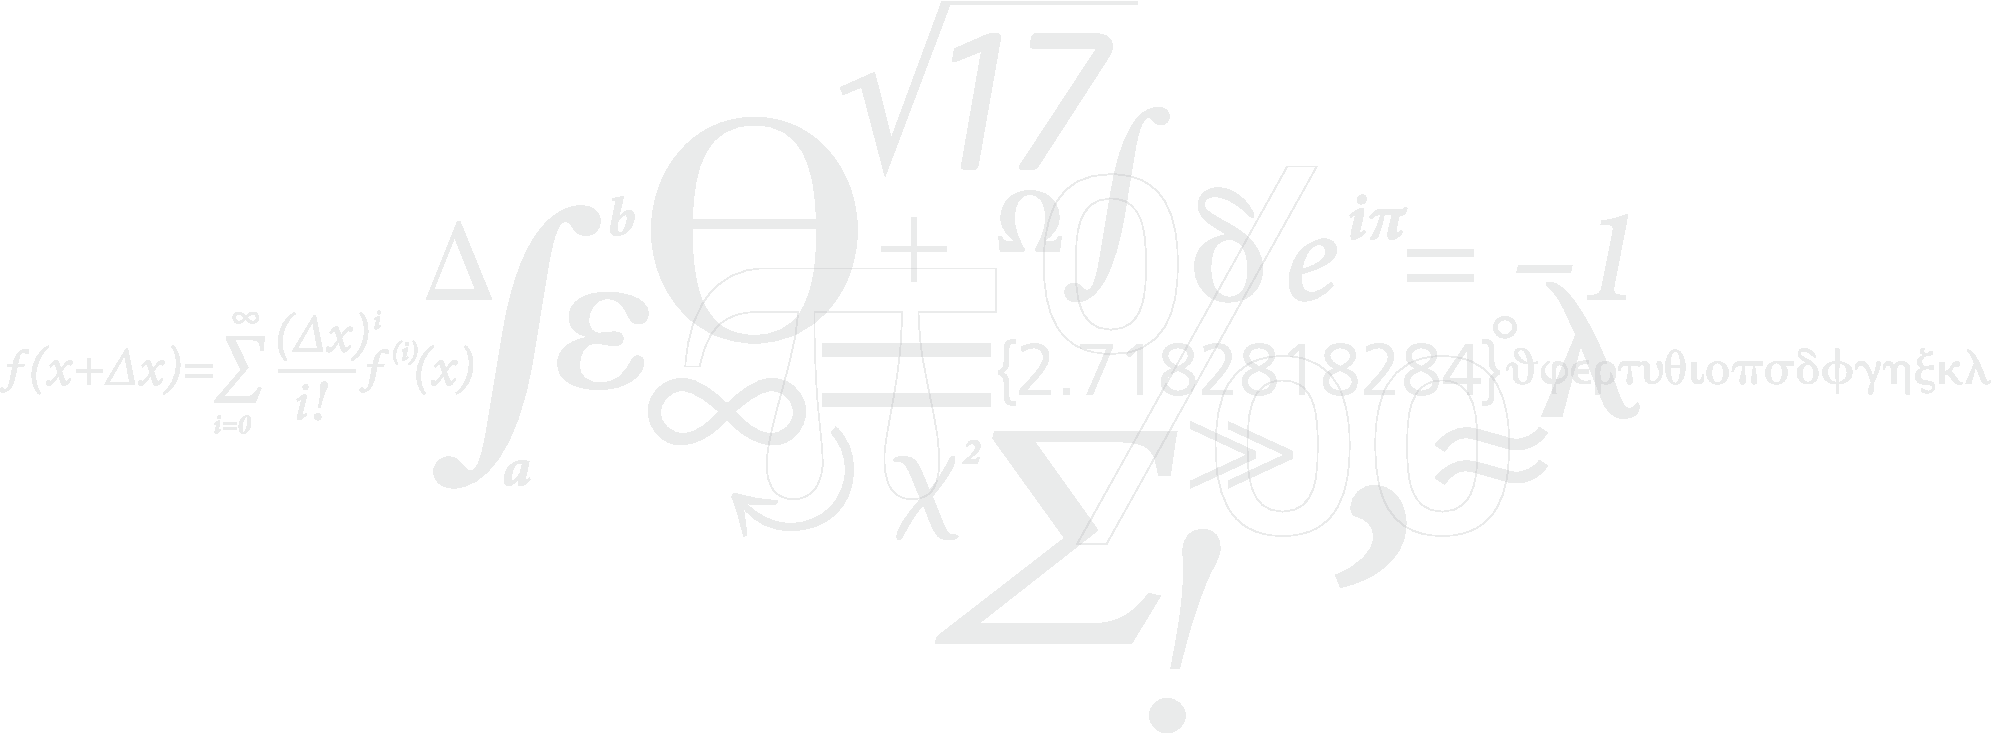
\includegraphics[trim=130mm 0 0 0,width=0.9\textwidth]{DTU-frise-SH-15}
                \vspace*{2.5cm}
            }
        }
    }
}

% This is a double sided book. If there is a last empty page lets use it for some fun e.g. the frieze.
% NB: For a fully functional hack the \clearpage used in \include does some odd thinks with the sequence numbering. Thefore use \input instead of \include at the end of the book. If bibliography is used at last everything should be ok.
\makeatletter
% Adjust so gatherings is allowd for single sheets too! (hacking functions in memoir.dtx)
\patchcmd{\leavespergathering}{\ifnum\@memcnta<\tw@}{\ifnum\@memcnta<\@ne}{
    \leavespergathering{1}
    % Insert the frieze
    \patchcmd{\@memensuresigpages}{\repeat}{\repeat\frieze}{}{}
}{}
\makeatother

%!TEX root = ../Thesis.tex

% Text fonts (http://www.macfreek.nl/memory/Fonts_in_LaTeX)
% Install fonts from /usr/local/texlive/<version>/texmf-dist/fonts/opentype/public
\usepackage{fontspec}

% Sans-serif font
\setsansfont[
    Ligatures=TeX,
    Extension=.otf,
    UprightFont=*-regular,
    BoldFont=*-bold,
    ItalicFont=*-italic,
    BoldItalicFont=*-bolditalic,
    %SlantedFont=,
    %BoldSlantedFont=,
    %SmallCapsFont=
    Scale=0.8      % Adjustmens when using math in sections
]{texgyreadventor}
%\setsansfont[Ligatures=TeX]{Neo Sans Intel}    % Neo Sans Intel – Like DTU font but more symbols
%\setsansfont[
%    Ligatures=TeX,
%    Scale=0.8
%]{NeoSans}           % NeoSans – DTU font (missing `+' symbols and other)
%\setsansfont[Ligatures=TeX]{CMU Sans Serif}    % Computer Modern Unicode font
%\setsansfont[Ligatures=TeX]{Latin Modern Sans} % Latin Modern Sans serif font

% Use this for more convienent sans serif font in math mode.
%\setmathsf{Latin Modern Sans}


%!TEX root = ../Thesis.tex

% Content specific packages.
\usepackage{grffile}
\usepackage[final]{pdfpages}
\usepackage{blindtext}
\usepackage{algorithm}
\usepackage{algpseudocode}
\usepackage{tabularx}
\usepackage{breakcites}
\usepackage[withpage]{acronym}
\usepackage{amsmath}
%\usepackage{pgfplots}                 % Plot tools
%\usetikzlibrary{
%    arrows,
%    matrix,
%    positioning,
%    shapes,
%    topaths,
%}
%\pgfplotsset{compat=1.7}

% Listings
\lstset{
    basicstyle=\footnotesize\ttfamily,% the size of the fonts that are used for the code
    breakatwhitespace=false,          % sets if automatic breaks should only happen at whitespace
    breaklines=true,                  % sets automatic line breaking
    captionpos=b,                     % sets the caption-position to bottom
    commentstyle=\color{s14a},        % comment style
    deletekeywords={},                % if you want to delete keywords from the given language
    escapeinside={\%*}{*)},           % if you want to add LaTeX within your code
    frame=single,                     % adds a frame around the code
    keywordstyle=\bfseries\ttfamily\color{s09}, % keyword style
    language=Python,                  % the language of the code
    morekeywords={*,...},             % if you want to add more keywords to the set
    numbers=left,                     % where to put the line-numbers; possible values are (none, left, right)
    numbersep=5pt,                    % how far the line-numbers are from the code
    numberstyle=\sffamily\tiny\color{dtugray}, % the style that is used for the line-numbers
    rulecolor=\color{dtugray},        % if not set, the frame-color may be changed on line-breaks within not-black text (e.g. comments (green here))
    showspaces=false,                 % show spaces everywhere adding particular underscores; it overrides 'showstringspaces'
    showstringspaces=false,           % underline spaces within strings only
    showtabs=false,                   % show tabs within strings adding particular underscores
    stepnumber=1,                     % the step between two line-numbers. If it's 1, each line will be numbered
    stringstyle=\color{s07},          % string literal style
    tabsize=2,                        % sets default tabsize to 2 spaces
    title=\lstname,                   % show the filename of files included with \lstinputlisting; also try caption instead of title
}


\addbibresource{bibliography/MyPapers.bib}
\addbibresource{bibliography/Bibliography.bib}
\addbibresource{bibliography/DTW-Paper.bib}
\begin{document}

\prefrontmatter
%!TEX root = ../Thesis.tex 
\thispagestyle{empty}             % No page numbers
\calccentering{\unitlength}
\begin{adjustwidth*}{\unitlength}{-\unitlength}
    \begin{adjustwidth}{-0.5cm}{-0.5cm}
        \sffamily
        \begin{flushright}
            \thesistypeabbr{} Thesis\\*[0cm]
            \thesistype{}\\
        \end{flushright}
        \vspace*{\fill}
        \noindent
        
\includegraphics[width=0.75\textwidth]{fysik_uk}\\*[0.5cm]
        \HUGE \thesistitle{}\\*[0.2cm]
        \Huge \thesissubtitle{}\\*[1.2cm]
        \parbox[b]{0.5\linewidth}{%
            \LARGE 
            \thesisauthor{}\\*[1.2cm]
            \Large
            \thesislocation{} \the\year
        }
        \hfill
\includegraphics[scale=0.7]{DTU-logo-CMYK}
    \end{adjustwidth}
\end{adjustwidth*}
\normalfont
\normalsize

\cleartoevenpage
%!TEX root = ../Thesis.tex
\thispagestyle{empty} % No page numbers
\frieze
\vspace*{\fill}
\noindent
\sffamily
\small
\textbf{DTU Physics}\\
\textbf{Department of Physics}\\
\textbf{Technical University of Denmark}\\
\\
Fysikvej\\
Building 311\\
2800 Kgs. Lyngby, Lyngby\\ 
info@fysik.dtu.dk\\ 
Tel.: +45 4525 3344\\ 
https://www.fysik.dtu.dk\\
\normalsize
\normalfont
\vspace*{2.5cm}

\clearforchapter

\frontmatter
%!TEX root = ../Thesis.tex
\chapter{Abstract}
Machine Learning provides an important tool for the modelling and analysis of geoscientific data. I have placed recent developments in deep learning into the greater context of machine learning by prefacing my work with a comprehensive history of machine learning and have reviewed the approaches and challenges of the use of machine learning in geoscience specifically. I have compiled a synopsis of the following chapters that contain topical peer-reviewed papers. 

This thesis follows the full data science workflow, starting with familiarization of the data domain in one published journal article, one published conference paper and one published workshop paper. It is followed by groundwork on machine learning and data processing on 4D seismic data in two submitted journal articles, one published conference paper and one published workshop paper. Based on this groundwork, I present a method for 4D seismic inversion in two published workshop papers. Finally, I present a novel unsupervised 3D time-shift extraction method for 4D seismic in one submitted journal paper. 

The aim of this thesis is to apply recent developments in computer vision systems and neural networks to physical data, particularly 4D seismic analysis. Neural networks are a type of machine learning that has made significant contributions to modern artificial intelligence and automatization. The applicability of neural networks for their capability of being a universal function approximator was recognized within geophysics from an early stage. With the deep learning boom, neural networks have experienced a renaissance in geoscience applications, particularly automatic seismic interpretation, inversion processes and sequence modelling.

The data for this thesis was acquired in the Danish North Sea, which contains chalk deposits, a sedimentologically distinct feature in the seismic data. The hydrocarbon-reservoir within the chalk has been subject to well-log analysis and core sampling in addition to seismic interpretation and 4D seismic analysis. During familiarization with the data, a new method to delineate chalk sediment in back-scatter scanning electron microscopy is introduced. Moreover, core fracture patterns, well imaging and seismic data are analyzed and compiled into a new workflow to ensure alignment of local and regional stress regimes.

Considering the wide interest in machine learning, my research investigates the following assumptions. The first paper shows that using pre-trained neural networks on natural images can reduce the data necessary for transfer learning to geoscience problems. I go on to analyze aliasing in neural networks and built a framework for complex-valued convolutional and dense neural networks to test the assumption that phase information can be implicitly learnt by real-valued neural networks. I further show that complex-valued convolutions can stabilize training and data compression on non-stationary physical data.

During the external research stay, a collaboration with an expert on Bayesian inversion for pressure-saturation inversion from 4D seismic amplitude difference maps resulted in a novel deep dense sample-based encoder-decoder network that learns the inversion process. The network contains a low-assumption physical basis (AVO) and learns the residual for the inversion process. My work shows that transfer from simulation data to field data is possible.

Finally, an unsupervised method is devised to extract 3D time-shifts from two 4D seismic cubes. The network extracts these 3D time-shifts with the inclusion of uncertainty measures. Commonly, time-shifts are extracted in 1D, due to processing speed, computational cost and poor performance of 3D methods. Within the training loop, the stationary velocity field is numerically integrated to obtain a diffeomorphic warp field that constrains the topology in a geologically consistent manner. The unsupervised implementation of the network structure ensures that biases from other time-shift extraction methods are not implicitly included in the network.

Overall, this thesis presents two new methods for the application of deep learning in 4D seismic analysis. Moreover, this thesis dives into information-theoretical implications of neural networks for non-stationary data such as seismic, and presents several ways to apply deep learning in a data regime, where ground truth is expensive, sparse, and sometimes impossible to obtain. These include transfer learning of pre-trained networks and transfer from simulation to field data. Additionally, we show an application of unsupervised learning, by devising a way of behaviour for the network to follow instead of supplying ground truth labels. Moreover, this results in a way to increase trust in the system, by limiting the extraction process to the deep learning system and performing well-defined operations within the network to automate the training, therefore, making the process transparent.


\chapter{Dansk Resum\'e}
Maskinl{\ae}ring (’machine learning’) er et vigtigt redskab til modellering og analyse af geovidenskabelige data. Jeg har sat den seneste udvikling inden for dyb l{\ae}ring (’deep learning’) ind i en st{\o}rre sammenh{\ae}ng via et forord, der gennemg{\aa}r maskinl{\ae}ringens historie, samt metoderne til og udfordringerne ved brug af maskinl{\ae}ring, specifikt inden for geovidenskab. Afhandlingen best{\aa}r af en synopsis af de publicerede og indsendte peer-reviewed afhandlinger i de derefter f{\o}lgende kapitler. 

Denne afhandling starter med at give overblik over af data via en publiceret tidsskriftsartikel, en publiceret konferenceartikel og en publiceret workshopartikel. Dern{\ae}st f{\o}lger forarbejdet til maskinl{\ae}ring og databehandling af 4D seismiske data i to indsendte tidsskriftsartikler, en publiceret konferenceartikel og en publiceret workshopartikel. P{\aa} baggrund af dette forarbejde, pr{\ae}senterer jeg en metode til 4D seismisk inversion i to publicerede workshopartikler. Endelig pr{\ae}senterer jeg en ny, 3D ekstraktionsmetode med tidsforskydning (’time shift’) for 4D seismiske data med brug af unsupervised learning i en indsendt tidsskriftartikel. 

Form{\aa}let med denne afhandling er, at anvende den seneste udvikling inden for systemer for computer vision og neurale netv{\ae}rk for fysiske data, is{\ae}r 4D seismisk analyse. Neurale netv{\ae}rk er en type maskinl{\ae}ring, der har bidraget stort inden for moderne, kunstig intelligens og automatisering. Det blev p{\aa} et tidligt tidspunkt anerkendt inden for geofysik, at neurale netv{\ae}rk var anvendelige. Med fremgangen inden for dyb l{\ae}ring, har neurale netv{\ae}rk oplevet en ren{\ae}ssance inden for geovidenskabelige anvendelser, is{\ae}r automatisk seismisk tolkning, inversionsprocesser og sekvensmodellering.

Data til denne afhandling, er indhentet fra den danske del af Nords{\o}en, der indeholder kridtaflejringer, hvilket er et sedimentologisk distinkt udtryk i de seismiske data. Kulbrinte-reservoiret i kridtet har v{\ae}ret genstand for borehulsanalyse og kernepr{\o}vetagning samt seismisk tolkning og 4D seismisk analyse. I forbindelse med arbejdet blev en ny metode til afgr{\ae}nsning af kridtsediment i scanning-elektronmikroskopi med tilbagespredning (’BSEM’) introduceret. Desuden blev kernefrakturm{\o}nstre, borehulsbilleder og seismiske data analyseret og samlet i en ny arbejdsgang for at justere lokale- og regionale stressregimer.

Set i lyset af den store interesse for maskinl{\ae}ring, unders{\o}ger min forskning flere omr{\aa}der. Den f{\o}rste artikel viser, at brugen af tr{\ae}nede neurale netv{\ae}rk p{\aa} billeder, kan reducere de data, der er n{\o}dvendige for at overf{\o}re l{\ae}ring til geovidenskabelige problemer. Jeg forts{\ae}tter med at analysere aliasing i neurale netv{\ae}rk og udvikler et computerprogram til at bygge neurale netv{\ae}rk, som bruger komplekse tal. Jeg sammenligner dette med netv{\ae}rk, som kun bruger ikke-komplekse tal, for at teste gendannelse af data og datakomprimering af ikke-station{\ae}re fysiske data.

Under det eksterne forskningsophold kom et samarbejde i stand, der udarbejder et nyt dybt, t{\ae}t pr{\o}vebaseret indkoder-dekoder-netv{\ae}rk, der l{\ae}rer inversionsprocesser. Netv{\ae}rket indeholder et fysisk grundlag, for selv at l{\ae}re resten af inversionsprocessen. Mit arbejde viser, at overf{\o}rsel fra indhentet data til simulationsdata er muligt.

Endelig blev der udviklet en ’unsupervised’ metode, til at udregne 3D-tidsforskydninger fra to 4D seismiske kuber. P{\aa} grund af de beregningsm{\ae}ssige omkostninger og d{\aa}rlige kvalitet, bliver disse normalt kun beregnet i 1D. Det neurale netv{\ae}rket beregner 3D tidsforskydningerne inklusiv usikkerhedsm{\aa}linger og er brugt p{\aa} tre forskellige seismiske datas{\ae}t. Den ’unsupervised’ implementering af netv{\ae}rksstrukturen sikrer, at bias fra andre tidsforskydnings ekstraktionsmetoder ikke implicit indg{\aa}r i netv{\ae}rket.

Samlet set, pr{\ae}senterer denne afhandling nye metoder inden for anvendelsen af dyb l{\ae}ring i 4D seismisk analyse. Desuden ser afhandlingen p{\aa} de informationsteoretiske konsekvenser af neurale netv{\ae}rk til ikke-station{\ae}re data, s{\aa}som seismik, og pr{\ae}senterer flere m{\aa}der at anvende dyb l{\ae}ring p{\aa} i et dataregime, hvor faktiske data er dyre at indsamle, af d{\aa}rlig kvalitet og nogle gange umulige at fremskaffe. Disse inkluderer overf{\o}rsel af l{\ae}ring i pr{\ae}-tr{\ae}nede (’pre-trained’) netv{\ae}rk og overf{\o}rsel fra simulationsdata til m{\aa}lt/indsamlet data.
%!TEX root = ../Thesis.tex
\chapter{Preface}
This xxx thesis was prepared at the department of Applied Mathematics and Computer Science at the Technical University of Denmark in fulfillment of the requirements for acquiring a yyy degree in zzz.

\vfill

{
\centering
    \thesislocation{}, \today\\[1cm]
    \hspace{3cm}
\includegraphics[scale=0.4]{Signature}\\[1cm]
\begin{flushright}
    \thesisauthor{}
\end{flushright}
}
%!TEX root = ../Thesis.tex
\chapter{Acknowledgements}

% Mikael
% Anders
% Colin

% Marie Daphne
% Toni

% Kirstie
% Anna

% Tim
% Matze
% Manuela
% Brian

% Florian
% Tala
% Fred

% Swung
% Lukas
% Matt
% Rob
%!TEX root = ../Thesis.tex
\chapter{Publication List}
\begin{refsection}

\nocite{*}
\newrefcontext[sorting=ynt]
\printbibliography[keyword={meins}, type=article, title={Journal Articles}, heading=subbibliography]

\printbibliography[keyword={meins}, keyword={conference}, type=inproceedings, title={Peer-Reviewed Conference Proceedings}, heading=subbibliography]

\printbibliography[keyword={meins}, keyword={workshop}, type=inproceedings, title={Peer-Reviewed Workshop Proceedings}, heading=subbibliography]

\printbibliography[keyword={meins}, keyword={other}, title={Not Peer Reviewed}, heading=subbibliography]
\end{refsection}

%!TEX root = ../Thesis.tex
\chapter{Presentation List}
\begin{refsection}[bibliography/MyPapers.bib]

\renewcommand*{\mkbibnamegiven}[1]{%
  \ifitemannotation{highlight}
    {\textbf{#1}}
    {#1}}

\renewcommand*{\mkbibnamefamily}[1]{%
  \ifitemannotation{highlight}
    {\textbf{#1}}
    {#1}}

\nocite{*}
\newrefcontext[sorting=ydnt]

\printbibliography[keyword={presentation}, keyword={meins}, keyword={conference}, type=inproceedings, title={Conference Presentation}, heading=subbibliography]

\printbibliography[keyword={presentation}, keyword={meins}, keyword={workshop}, type=inproceedings, title={Workshop Presentation}, heading=subbibliography]

\printbibliography[keyword={poster}, keyword={meins}, keyword={conference}, type=inproceedings, title={Conference Poster}, heading=subbibliography]

\printbibliography[keyword={poster}, keyword={meins}, keyword={workshop}, type=inproceedings, title={Workshop Poster}, heading=subbibliography]

\printbibliography[keyword={presentation}, keyword={other}, keyword={meins}, notkeyword={invited}, title={Other Presentations}, heading=subbibliography]

\printbibliography[keyword={poster}, keyword={other}, keyword={meins}, title={Other Posters}, heading=subbibliography]

\printbibliography[keyword={invited}, keyword={meins}, keyword={other}, title={Invited Presentation}, heading=subbibliography]

\renewcommand*{\mkbibnamegiven}[1]{%
  \ifitemannotation{highlight}
    {#1}
    {#1}}

\renewcommand*{\mkbibnamefamily}[1]{%
  \ifitemannotation{highlight}
    {#1}
    {#1}}

\end{refsection}

\clearforchapter
\tableofcontents
\clearforchapter
\mylistoftodos

\mainmatter
%!TEX root = ../Thesis.tex
\chapter{Introduction}


%!TEX root = ../Thesis.tex
\chapter{Methods \& Theory}
\todo{Write about Self-Supervision Extensively}

\todo{Talk about metrics and norms!}
% Geoscience
\todo{Write geoscience intro}

% 4D Seismic
\section{4D seismic}

4D seismic is the analysis of seismic data that was acquired over the same location after some calendar time has passed. The repeated imaging of the same subsurface location, highlights changes in the subsurface that can lead to improved understanding of subsurface processes and fluid movement. E\&P companies in particular have an interest in imaging hydrocarbon reservoirs \citep{Johnston2013-jg}, however 4D seismic imaging wide applications for subsurface characterization, such as observing volcanic activitiy \citep{londono20184d} or CO2 sequestration monitoring \citep{Arts2004-ym}. 

The main applications of 4D seismic analysis according to \citet{Yilmaz2003-hp,Johnston2013-qg} include:
\begin{itemize}
\item Tracking fluid movement (steam, gas, and water)
\item Monitoring pressure depletion and validating depletion plans
\item Fault property estimation i.e. sealing or leaking faults
\item Locating Bypassed oil imaging in heterogeneous reservoirs
\item Validating and updating geological and reservoir-simulation models
\end{itemize}

4D seismic data analysis suffers from the superposition of multiple effects on the seismic imaging. These effects include changes in the acquisition equipment due to technological advances, changes in acquisition geometry (source-receiver mismatch), as well as physical changes in the subsurface \citet{Yilmaz2003-hp, Johnston2013-jg}. These physical changes are in part due to fluid movement in the subsurface \citep{lumley1995seismic}, as well as, changes in the geology due to compaction and expansion \citep{Hatchell2005-op}. These geomechanical effects change the position of the reflectors, the thickness of stratigraphy and the physical properties such as density and wave velocity \citep{Herwanger2015-qz}.

Succesfull 4D applications rely on careful acquisition planning, closely matching the mismatch of source ($\Delta S$) and receiver ($\Delta R$). This awareness has generally improved the repeatability of seismic acquisition, however, the \ac{nrms} remains to be an important measure of noise sources that deteriorate the 4D seismic analysis. Moreover, 4D seismic analysis has brought to light that some 3D seismic processing workflows are not as repeatable and amplitude-preserving as they were thought to be \citep{Lumley2001-kx}. Modern processing flows include co-processing of the base and monitor seismic volumes with specialized tools to reduce differences from processing \citep{Johnston2013-qg}.

% Amplitude Differencing
% Time Shift Analysis
The standard analysis tool in 4D seismic interpretation are amplitude differences \citep{Johnston2013-jg}. Differences can stem from fluid movement or replacement and changes in the rock matrix due to compaction or temperature changes. Additionally, by-passed oil zones in heterogeneous reservoirs can be identified by "low difference zones" in generally mobile reflector packets \citep{Yilmaz2003-hp}. Usually, a simple difference of the 3D seismic volumes will not yield satisfactory results due to small-scale fluctuations in both arrival times and amplitudes, making time-shift analysis an important process to match the reflection events. These time-shift values have been shown to be a valuable source of information themselves \citep{Hall2002-dt,Hatchell2005-eg}, considering their sole dependence on wavefield kinematics, time shifts tend to be a more robust measurement than amplitude differences \citep{Johnston2013-jg}.

Considering normal incidence on a horizontal layer of thickness $z$ and a P-wave velocity $v$ with a traveltime $t$, we can express the changes in traveltime as:

\begin{equation}
    \frac{\Delta t}{t} = \frac{\Delta z}{z} - \frac{\Delta v}{v},
    \label{eq:timestrain}
\end{equation}

for homogeneous isotropic $v$ and small changes in $z$ and $v$. Originally developed in \citet{Hatchell2005-eg}, with a rigorous integral derivation presented in \citet{macbeth2019post}.

The vertical strain $\frac{\Delta z}{z}$ directly relates to the geomechanical strain $\epsilon_{zz}$, describing the vertical strain on the vertical surface of a infinitesemal element \citep{Herwanger2015-qz}. Independently \citet{Hatchell2005-eg} and \citet{roste2006estimation} developed a single-parameter solution to relate velocity changes and vertical strain

\begin{equation}
    \frac{\Delta v}{v} = - R \epsilon_{zz}
    \label{eq:R}
\end{equation}
with $R$ being the single parameter \ac{hbr} \citep{Hatchell2005-op, macbeth2019post}. The \ac{hbr} being a lithological constant, we can relate \cref{eq:R} and \cref{eq:timestrain} and obtain a direct relationship between the vertical strain $\epsilon_{zz}$ and the time shift $\Delta t$ for a given lithology with property $R$

\begin{equation}
    \Delta t = t \cdot (1 + R) \cdot \epsilon_{zz}.
\end{equation}

Contingent on the assumption of zero-offset incidence, homogeneous velocity and isotropy, time shift extraction is mostly performed in z-direction by comparing traces directly. Prominently, the 1D windowed cross-correlation is used due to its computational speed and general lack of limiting underlying assumptions \citep{Rickett2001-nx}. The main drawback of this method is, however, that the result is highly dependent on the window-size and susceptible to noise. Other methods for post-stack seismic time shift extraction include \ac{dtw} \citep{Hale2013} and inversion-based approaches \citep{Rickett2007-yo}. 

More recently research into pre-stack time shift extraction and 3D-based methods is conducted. These methods relax the constraints of some assumptions of 1D applications \citep{ghaderi2005pre, hall2002time}. 3D time shifts have the ability to capture subsurface movement of reflectors and account for 3D effects of the $\Delta R / \Delta S$ acquisition mismatch, which effect seismic illumination.

\acf{qi} extends the interpretation of 4D changes to estimate fluid saturation and pressure changes within the reservoir. The subsurface changes recorded by the seismic data can be related to subsurface changes. These changes include fluid saturation and pressure changes, with the inversion process being non-unique and often reliant on prior information. The decoupling of pressure and saturation changes is non-trivial and relies on pre-stack or angle-stack information \citep{Landro2001-rz}.

Active areas of research in 4D seismic are the use of 4D seismic data to estimate saturation and pressure changes quantitatively particularly in volumetric applications as opposed to map-based approaches. However, these approaches often depend on reliable rock-physics models, an area of research in model-based approaches. Moreover, there's active research in moving to volumetric approaches in time-shift estimation and quantitative pre-stack analysis. Additional research in extractive data-based methods and model-based approaches investigate how much information is available directly from the data and what information is available from the modelling feedback-loop.

\section{Machine Learning}
%\todo{Write machine learning intro}
\acf{ml} is the discipline of defining a statistical or mathematical models based on data. These \ac{ml} models are either trained in a supervised or unsupervised fashion, which usually results in them learning a decision boundary, or a representation or structure of the data respectively. Historically, \ac{ml} has been an interest in geoscience but has not gained momentum due to sparse data, computational capability, and availability of algorithms. Geoscience data was often not available and still is often not available with a reliable ground truth. However, particularly \acp{nn} have found broad interest in geophysical applications, Bayesian methods are often used in inversion schemes and recent software developments have changed the research entirely.

% Development of Deep Learning
Recently, the subfield \ac{dl} has reignited interest in the wider field of \ac{ml} by outperforming rule-based algorithms on computer vision tasks, such as image classification and segmentation \citep{Bishop2016-mj}. These developments have propelled developments in other non-related fields such as biology \citep{Ching2018-hg}, chemistry \citep{Schutt2017-sh}, medicine \citep{Shen2017-nt} and pharmacology \citep{Kadurin2017-oq}. \ac{dl} utilizes many-layered artificial \ac{nn} to approximate an objective function. In recent years the open source movement, democratization of access to computing power and developments in the field of \ac{dl} have rekindled interest in applications of \ac{ml} to geoscience. The availability of free open source libraries such as skikit-learn \citep{scikit-learn} has made \ac{ml} methods and several tools for the application of rigorous statistical evaluation of experiments without explicit expert knowledge widely available. Furthermore, Tensorflow \citep{tensorflow}, PyTorch \citep{pytorch}, and Keras \citep{keras} have made \acp{nn} easily accessible and provide experimentation capabilities to transfer recent developments in \ac{ml} research to other scientific fields. 


Algorithms and methods in \ac{ml} can be organized in different ways. Two ways to categorize algorithms are based on the training or based on the learned distribution. In training, these algorithms can be categorized into supervised and unsupervised methods, where supervised methods learn the functional mapping from $x$, being the data, to $y$, being the ground truth or label for the data. When the ground truth is not known, unsupervised methods can be applied to determine structures and relationships within the data. Semi-supervised, and weakly supervised try to propagate partial labels to similarly distributed data and then learn the supervised mapping f(x) = y. Alternatively, \ac{ml} algorithms can be categorized into generative methods that learn the joint probability distribution or discriminative methods that learn a decision boundary to optimally separate data. Additionally, methods can be distinguished by application. Assigning labels to data is called classification. The general, continuous application to map data from the input to the output domain is called regression. Finding relationships and agglomerations of data is called clustering. Most algorithms can be applied to several of these categories, such as support vector machines that can function as classifier and regressor. 

Applications in \ac{ml} are quickly evolving and many are improved by mathematical insights, engineering features and increased availability of data. This thesis focuses on the application of \acp{nn}, which come in different implementation details and particularly \ac{nn} architectures are often re-implemented with slight differences that deviate from the original published architecture. Particularly in \ac{nn} we have to focus on the most practical building blocks, to be able to give a comprehensive overview.

\subsection{History of Machine Learning}

\begin{figure}[H]
    \centering
    \hspace*{-1.5cm}
    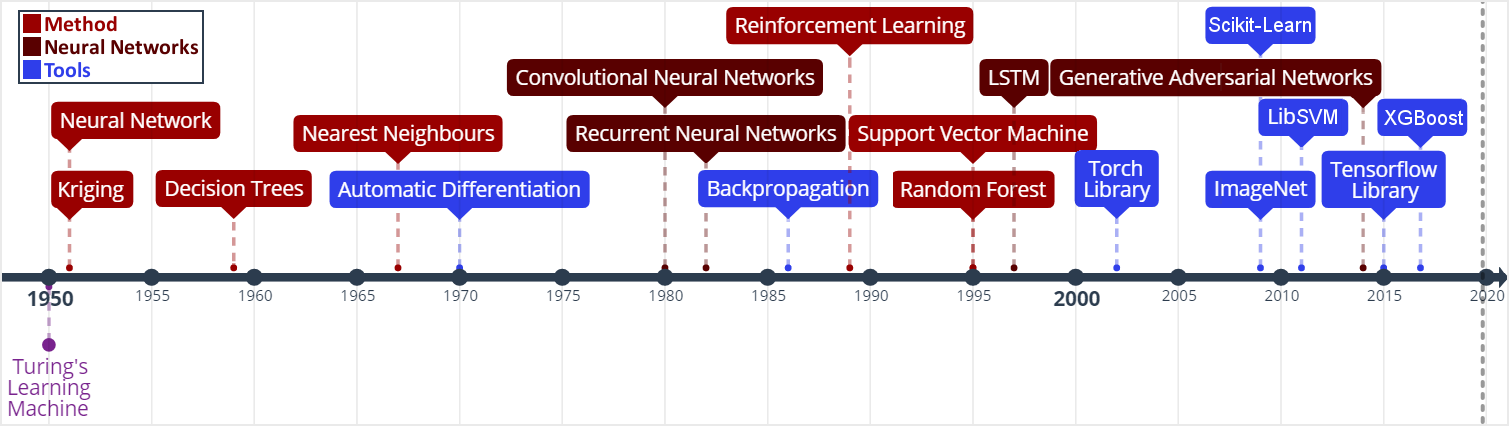
\includegraphics[width=1.15\textwidth]{figures/ML-Timeline.png}
    \caption{Selection of notable milestones in machine learning}
    \label{fig:mltimeline}
\end{figure}

Creativity, learning, and intelligence with regard to computers have been discussed as early as of the first programmer Ada Lovelace \citep{taylor1843scientific}.

\begin{quote}
    "The Anlytical Engine has no pretensions whatever to \textit{originate} any thing. It can do whatever we \textit{know how to order it} to perform. It can \textit{follow} analysis; but it has no power of \textit{anticipating} any analytical relations or truths. Its province is to assist us in making \textit{available} what we are already acquainted with. This it is calculated too effect primarily and chiefly of course, through its executive faculties; but it is likely to exert an \textit{indirect} and reciprocal influence on science itself in another manner." -- Note G, Page 689, Ada A. Lovelace. \citep{taylor1843scientific}; Emphasis taken from source text.
\end{quote}

This notion was challenged by Alan Turing \citep{turing1950} who proposed the "Learning Machine", which specifically predict genetic algorithms, a metaheuristic that finds application in optimization and search problems. Evolutionary computing and genetic algorithms specifically can perform some machine learning tasks \citep{Goldberg1988-ch}. This is generally considered the commencement of \ac{ai} and \ac{ml}, however, they rely heavily on earlier developments in statistics such as the Bayesian theorem \citep{bayes1763lii} and Markov processes \citep{markov1906rasprostranenie,markov1971extension}. The first method, we include on the timeline in \cref{fig:mltimeline} is "kriging" \citep{Krige1951}, which is based on Gaussian Processes, these form an important category of non-parametric machine learning these days. Gaussian processes are often also attributed to work of \citet{kolmogorov1939interpolation} on time series. Another method was developed to mimic the human brain, namely \acfp{nn}. The construction of the first \ac{nn} machine by Minsky \citep{russelnorvig} was soon followed by the "Perceptron", a binary decision boundary learner \citep{rosenblatt1958perceptron}. The decision is made according to

\begin{equation}
\begin{array}{ll}
    o_{j} & = \sigma \left(\sum_i w_{ij} x_{i} + b\right)\\
    & = \begin{cases}1&\sum_i w_{ij} x_{i} + b > 0 \\ 0 &\text{otherwise}   \end{cases}
\end{array}
\end{equation}
which describes a linear system of the input data $x$, the weights $w$ and bias $b$ and a binary activation funtion $\sigma$. The linear system is still used in modern neurons, however, the activation $\sigma$ is usually a Rectifier function. Shortly after, \citet{belson1959matching} describe the first \acf{dt}, which learns hierarchical decision systems. The next method, \ac{knn} search, was introduced by \citet{cover1967nearest} to solve the traveling salesman problem. Two decades later Q-learning \citep{watkins1989learning} introduces a method to reinforcement learning that is still used to this day. The final two methods in the timeline were introduced in 1995. \acfp{rf} \citep{ho1995random} introduce ensemble learning of weak learning \acfp{dt}. \acf{svm} \citep{cortes1995support} introduce a strong learner that aims to maximize the margin between classes.

These methods have been improved upon over the decades. Specific milestones that accelerated further developments in \ac{nn} are automatic differentiation \citep{linnainmaa1970representation} and consequently applying this to backpropagate errors in \acp{dnn} \citep{rumelhart1988learning}. Backpropagation itself as a concept existed earlier \citep{kelley1960gradient, bryson1961gradient}, followed by a simplification by using the chain rule \citep{dreyfus1962numerical}. These enable effective implementation of \acp{nn} today. Moreover, open sourcing the Torch library \citep{collobert2002torch} made and assembling the ImageNet database \citep{deng2009imagenet} has accelerated developments in computer vision and enabled modern developments in deep learning. In the same year of 2009 the library Scikit-Learn \citep{scikit-learn} was established, which introduced a common open source \ac{api} \citep{sklearn_api} for a diverse and growing set of shallow machine learning models (e.g. \acp{svm}, \acp{rf}, \acp{knn}, shallow \acp{nn}). Scikit-learn has had a profound impact on machine learning applications across the sciences and the API is modelled in other open source libraries. \citet{libsvm} introduced a widely used implementation for \acf{svm}, which is also used in Scikit-Learn. Recently, the Tensorflow library \citep{tensorflow} was introduced for open source deep learning models, with some different design choices than Pytorch. In this open environment fueled by competitions (e.g. ImageNet \citep{ILSVRCanalysis_ICCV2013}, Netflix Prize \citep{bennett2007netflix}, Kaggle \citep{goodfellow2013challenges}) XGBoost \citep{xgboost}, a library for extreme gradient tree boosting was developed.

Recent developments in deep learning are based in \acfp{nn}, hence, we highlight some key developments in \cref{fig:mltimeline}. \acfp{cnn} are essential in the modern computational vision systems, they were inspired by the concept of Neocognitron \citep{fukushima1980neocognitron, lecun2015deep}. In the same decade \acfp{rnn} were introduced implemented as Hopfield Networks \citep{hopfield1982neural}. While Hopfield networks are not a general \ac{rnn}, they provide content-adressable memory with the internal state memory. \citet{hochreiter1997long} implement the \acf{lstm}, which contain internal states (i.e. memory) that can process temporal sequences, still used and performing to the state-of-the-art in sequence analysis and \ac{nlp} to this day. Recently, \acf{gan} \citep{goodfellow2014generative} introduced a system of \acp{nn} that can create new samples from a distribution. The \ac{gan} consists of two \acp{nn}, a generator and a discriminator, which generate samples from a noise distribution and judge the validity of the sample respectively. We discuss \acp{nn} in more detail in \cref{section:nn}

\subsection{\acfp{nn}}
\label{section:nn}
\acf{nn} as a class of \ac{ml} algorithms are very diverse and versatile. \acp{nn} have persisted for decades and their nomenclature has changed in this time. \acp{nn} were long called \ac{ann}, which has changed to simply \ac{nn}, usually prepended with the class of \acl{nn}, namely  \acf{rnn}, \acf{cnn}, \acf{dnn}, which I will discuss in more detail.

\begin{figure}[H]
    \centering
    \includesvg[width=\textwidth,height=5cm]{{figures/Single-Layer_Neural_Network}}
    \caption{A simple \ac{nn} \todo{More text}}
    \label{fig:simpleneuralnetwork}
\end{figure}

\acfp{nn} can be approached from several theoretical bases. Mathematically, \acp{nn} are directed acyclical graphs with edges and nodes. In neural computation, these are generally referred to as weights and nodes or neurons. In \cref{fig:simpleneuralnetwork}, we present a simple densely connected \ac{mlp} with three inputs and three outputs. This configuration is equivalent to a linear regression model. The inputs are distributed across the nodes, and each weight is multiplied with a weight inherent to that graph edge. During the training of this machine learning model, these weights get adjusted to obtain a generalizable result. Each node sums the contributions of these weights and possibly a bias, which is trainable but does not take input data. This amounts to each node performing

\begin{equation}
    a_{j} = \sigma \left(\sum_i w_{ij} x_{i} + b\right),
\end{equation}
with $a$ signifying the activation at a node, $i,j$ being the index of the source and target node respectively, $w$ being the trainable weight, and $b$ being the trainable bias, and $\sigma$ representing an activation function. Activation functions are an active topic of research, but the generally perform a non-linear transformation of the activation at the node.

\begin{figure}[H]
    \centering
    \subbottom[Linear activation]{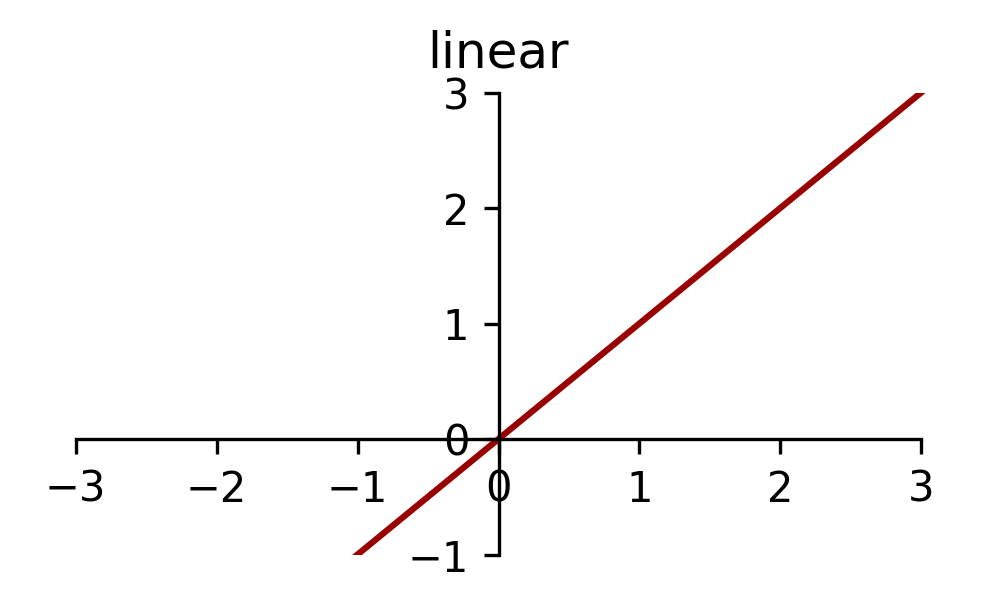
\includegraphics[width=.35\textwidth]{figures/activations/act_linear.png}\label{fig:act_lin}}%
    \subbottom[Sigmoid activation]{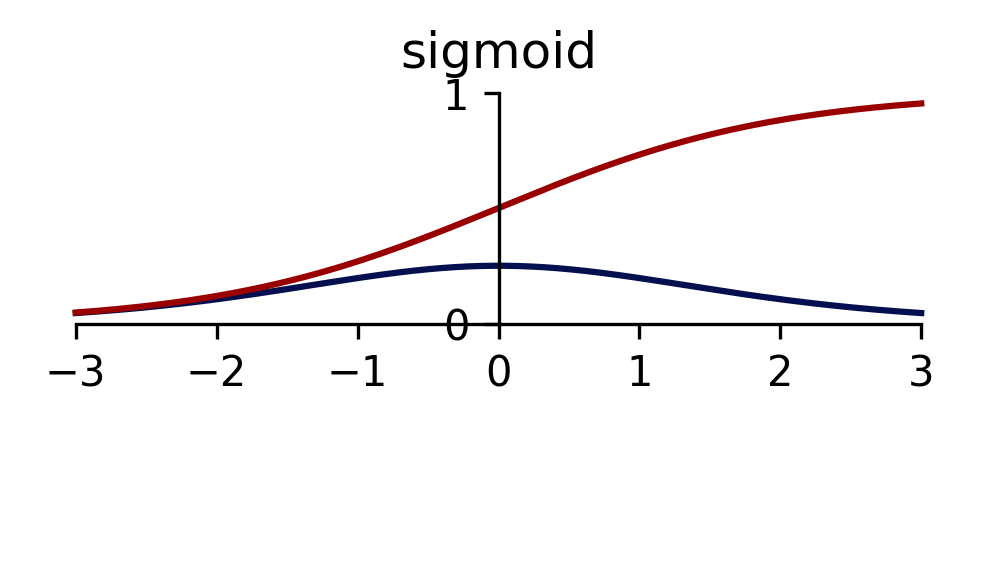
\includegraphics[width=.35\textwidth]{figures/activations/act_sigmoid.png}\label{fig:act_sig}}%
    \subbottom[Tanh activation]{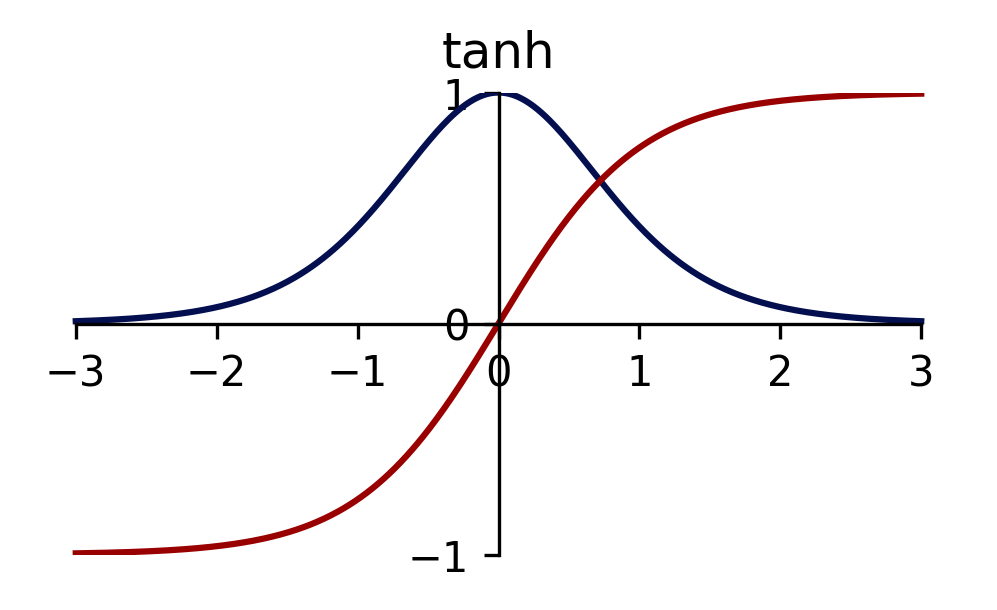
\includegraphics[width=.35\textwidth]{figures/activations/act_tanh.png}\label{fig:act_tanh}}%
    \\
    \subbottom[\ac{relu} activation]{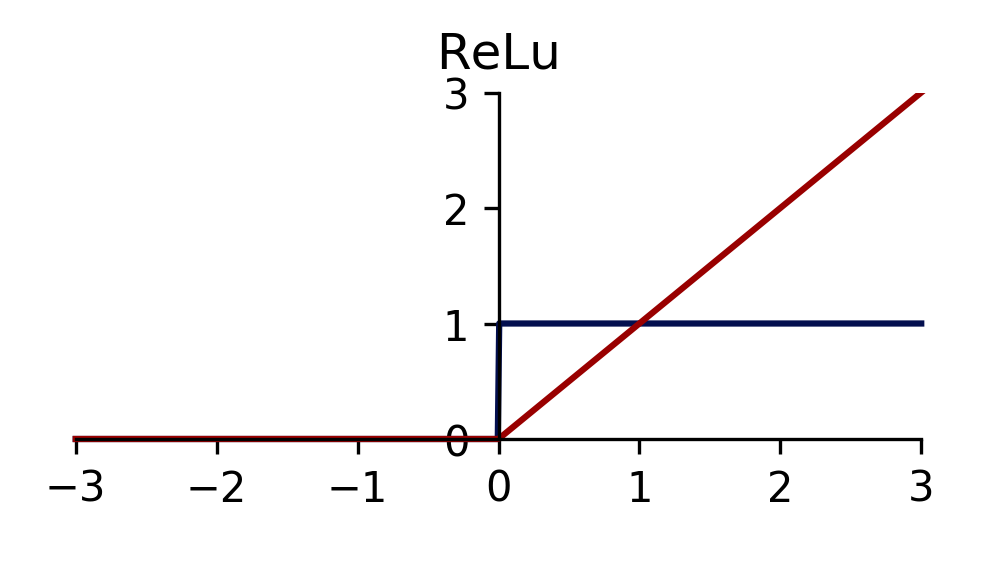
\includegraphics[width=.35\textwidth]{figures/activations/act_relu.png}\label{fig:act_relu}}%
    \subbottom[\ac{prelu} activation ($\alpha=.5$)]{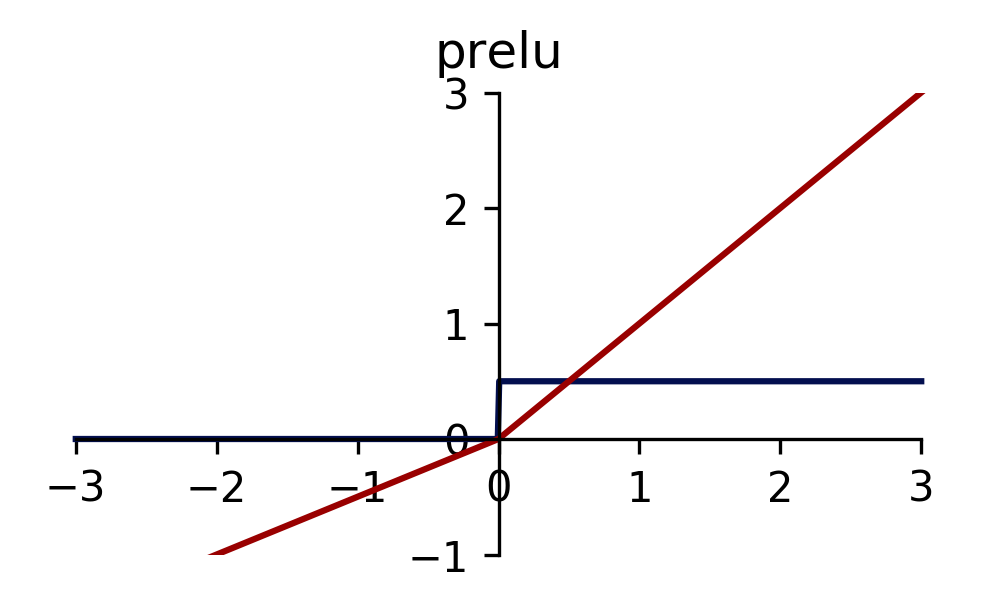
\includegraphics[width=.35\textwidth]{figures/activations/act_prelu.png}\label{fig:act_prelu}}%
    \subbottom[\ac{elu} activation ($\alpha=1$)]{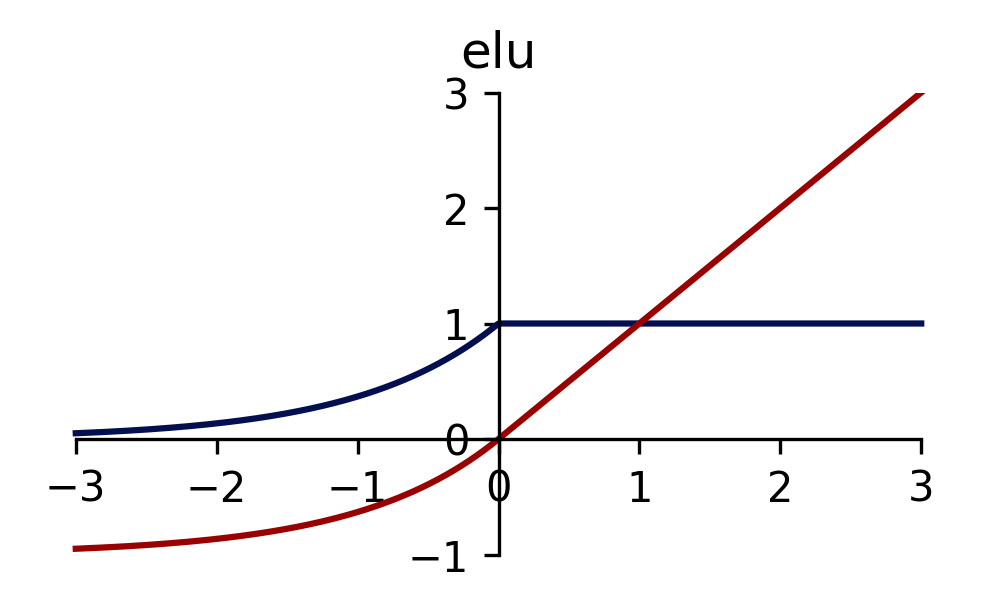
\includegraphics[width=.35\textwidth]{figures/activations/act_elu.png}\label{fig:act_elu}}
    \caption{Common Activation functions (red) and derivatives (blue)}
    \label{fig:activations}
\end{figure}

In \cref{fig:activations} I present common activation functions used in \acp{nn}. The activation functions introduce non-linearities into the network to transform the linearly scaled input to arbitrary non-linear outputs. The mathematical function in \cref{fig:act_sig} and \cref{fig:act_tanh} are used less, because of the vanishing gradient problem \citep{hochreiter1991untersuchungen}. These occur in the extrema of both functions, where the function saturates and the gradient is close to zero for large values of x. Rectifiers presented in \cref{fig:act_relu,fig:act_prelu,fig:act_elu} circumvent this problem by one-sided saturation. 

\paragraph{Training the Model} 
Before training, each weight and bias is assigned an initial number that is drawn from a distribution appropriate to the network architecture and data \citep{lecun2012efficient, glorot2010understanding, he2015delving}. These strategies collectively initialize weights in a pseudo-random way within limits. The data is then passed through the network, which calculates a result. This result is then compared to the ground truth, using a loss function (e.g. \ac{mae}, \ac{mse}). The resulting error $\Delta t$ is then used to correct the weights and biases in the network, calculating the correction per weight $\Delta w_{ij}$ recursively (for many-layered networks).
\begin{equation}
    \Delta w_{ij}= -\eta \dfrac{\partial E}{\partial w_{ij}} = -\eta \delta_{j} a_{i},
\end{equation}
with $\eta$ being the learning rate and $\delta$ being
\begin{equation}
    \delta_{j}=\begin{cases}
\sigma'( \text{net}_{j} ) \Delta t              & \text{if } j \text{ is output node,}\\
\sigma'( \text{net}_{j} ) \sum_{j-1} \delta_{j-1} w_{j(j-1)} & \text{if } j \text{ is hidden node.}
\end{cases}
\end{equation}
Therefore, hidden nodes are reliant on the result $\delta_{j-1}$ of the node at index $j-1$ \citep{deeplearningbook}. The training of the model can be done on a per-sample basis, which is \ac{sgd} or in the case of noisy inputs, the mean error of several samples can be calculated to perform mini-batch gradient descent. Iteration over forward and backward passes adjusts the weights to predict the correct result. 

Modern deep \acp{nn} are trained on \acp{gpu} that are optimized for matrix multiplications instead of \acp{cpu} that are magnitudes slower. However, more recently task-specific hardware such as \acp{fgpa} and \acp{tpu}, which work closely with the \ac{tf} library are being developed and made available in cloud infrastructures.

The optimization of the backpropagation is performed using \ac{sgd} or other gradient-based optimizers such as the Adam optimizer \citep{kingma2014adam}. However, during training of the \ac{nn}, it is important to ensure that the network learns a general relationship instead of memorizing the input data. This memorization is called overtraining, or overfitting. Overfitting can be avoided by regularizations like weight decay \citep{krogh1992simple} and Nesterov momentum \citep{pmlr-v28-sutskever13}, which modify the optimization loop. Alternatively, methods like Dropout \citep{hinton2012improving} and \ac{bn} \citep{ioffe2015batch} modify the network at training time. Moreover, a diverse training set and train-val-test split help avoid overfitting and ensure generalization of the trained model.

The train-val-test split separates the data into three parts. The training and validation set are available during training and hyperparameter tuning, the test set, however, should only be used once to ensure generalization of the model. The train test is used during the optimization loop, the actual training of the model, with the validation set ensuring generalization of the model to unseen data within the loop. In and of itself, the train and validation data would be sufficient, if no other changes to the model were made based on the results of the validation data. Since hyperparameter tuning and model selection are a common procedure today, these present an implicit source of information leakage from the validation set into the data. The hyperparameter tuning will often pose an optimization loop in itself that optimizes based on the results on the "unseen" validation set, essentially implicitly fitting the model to the validation data, therefore, a separate test set is necessary to ensure true generalization.


\subsubsection{Feed Forward Networks}
Feed forward \acfp{nn} or \acp{mlp} are the simplest for of \ac{nn}. In its simplest form it uses a set of linear equations to approximate a function. The network can be described as a graph with edges and nodes. In the neural information community the nodes are often named neurons. These neurons are arranged into layers in \cref{fig:feedneuralnetwork}. The first layer in a \ac{nn} is the input layer with a number of nodes corresponding to the number of input data points. The input nodes are connected to the next layer by the graph's edge. The next node can be the output layer. The weights between subsequent are floating point numbers that scale each input point and determine the value at the output nodes.

\begin{figure}[H]
    \centering
    \includesvg[width=\textwidth,height=5cm]{{figures/Multi-Layer_Neural_Network-Vector}}
    \caption{Feed forward \ac{nn}}
    \label{fig:feedneuralnetwork}
\end{figure}

\acp{nn} gain their powerful learning capabilities from adding layers (see \cref{fig:feedneuralnetwork}) in between the input and output node and applying a non-linear activation function. Non-linear activations scale the input from the edge at each neuron. Historically, these have been straight-forward mathematical functions such as $tanh()$ and $sig()$ (cf. \cref{fig:activations}). These suffer from some short-comings that were overcome to leverage multi-layered \acfp{dnn}.

\subsubsection{\acfp{dnn}}
\label{section:dnn}
Improvements in computational power made it possible to train many-layered \acp{nn} (see \cref{fig:deepneuralnetwork}). These \acfp{dnn} are at the core of recent developments in \acf{dl}, leading to the re-implementation of many algorithms into openly available libraries, which has led to further innovative uses of these building blocks. These networks leverage the combinatorial power of \ac{nn} layers. In deep \acp{nn} gradient propagation led to exploding or vanishing gradients before. New non-saturating activation functions lead to stabilization of training \ac{dnn} (cf. \cref{fig:activations}).

\begin{figure}[H]
    \centering
    \includesvg[width=\textwidth,height=5cm]{{figures/Deep-Multi-Layer_Neural_Network-Vector}}
    \caption{Deep Feed forward \ac{nn}}
    \label{fig:deepneuralnetwork}
\end{figure}

\subsubsection{\acfp{som}}
\acf{som}, also named Kohonen-networks \citep{kohonen1982self} are a special case of networks that do not modify the flow of data from the input to the output nodes. They treat each data point as a node and adjust the weights between each node in on a similarity metric. These tend to perform well on spatially correlated data and find good adoption in geoscience.

\subsubsection{Recurrent Networks}
A special configuration of \ac{nn} is the \acf{rnn}. These networks use edges that feed back into the network. \acp{rnn} are used in two applications in \ac{ml}. They can preserve hidden states, which gives them temporal context sensitivity. Application two is time series analysis similar to feed-forward \acp{nn}, where the input is a time step that can be analyzed within the context of surrounding time steps. These \ac{rnn} represent cyclic directed graphs of computation, as opposed to the other types of \ac{nn} we discuss, which are acyclic directed graphs. 
In \cref{fig:recurrentneuralnetwork} we show the changes of a simple \ac{rnn} graph compared to a feed forward \ac{nn} in \cref{fig:feedneuralnetwork}. The \ac{rnn} loops back into itself, which is often regarded as the internal state or feedback. This internal state enables content addressable memory and good performance on sequential data such as time series and language.

\begin{figure}[H]
    \centering
    \includesvg[width=\textwidth,height=5cm]{{figures/Recurrent-Layer_Neural_Network-Vector-Blank}}
    \caption{Recurrent \ac{nn}}
    \label{fig:recurrentneuralnetwork}
\end{figure}

\paragraph{Hopfield Networks} are one type of recurrent networks that model the human memory. Hopfield networks and their subclasses can be used for pattern recognition. They are guaranteed to find a pattern, however, they are known to converge to local minima. Boltzman machines are configured like Hopfield networks, in contrast to deterministic Hopfield networks, their response to an input is stochastic. Boltzman machines draw from a joint distribution, making them a generative model.

\paragraph{\acf{lstm}} is a type of \ac{rnn} that models memory. Details differ in implementations of \acf{lstm}, however the main criteria are three gates and an inner cell. 
\begin{itemize}
    \item Input Gate
    \item Forget Gate
    \item Output Gate
\end{itemize}
The input gate regulates the contribution of input values to the internal cell. The forget gate regulates the persistence of values in the cell. Finally, the output gate regulates the contribution of the input value to the output value convolved with the cell state. 

\subsubsection{Convolutional Networks}
\label{section:cnn}
\acf{cnn} were developed in computer vision to automatically learn a filter that spatially correlates data. The convolutional kernels are computationally efficient due to weight sharing, making them feasible for very deep networks (cf. \cref{section:dnn}). \acp{cnn} have had the biggest influence on the renaissance of modern \ac{ml}. These building blocks for \acp{nn} are very good for image data and data where spatially correlated information provides valuable context. It has therefore quickly gained attention in seismic interpretation and seismic data analysis. CNNs like other \acp{nn} are optimized by \ac{sgd}, optimizing a defined loss over the chosen task.

\begin{figure}[H]
    \centering
    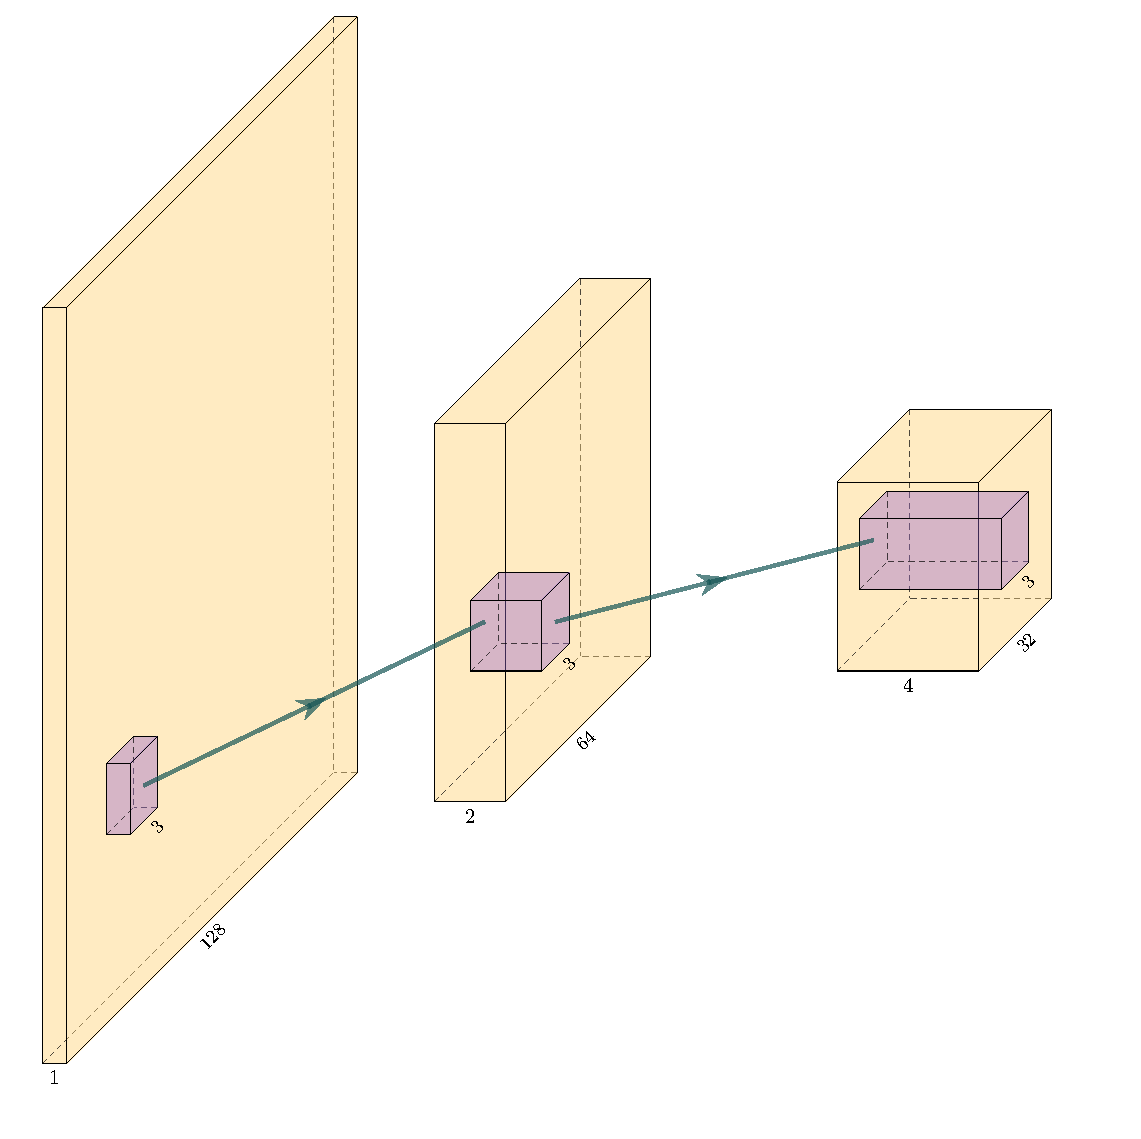
\includegraphics[width=\textwidth,height=5cm,keepaspectratio]{figures/cnn_schema.pdf}
    \caption{Schematic of a \ac{cnn} filter (purple) in the image data (orange)}
    \label{fig:cnn}
\end{figure}

For a two-dimensional \ac{cnn}, the convolution of the $m\times n$-dimensional image $G$ with a filter matrix $f$ can be expressed as:
\begin{equation}
G^{*}(x,y) = \sum_{i=1}^{n} \sum_{j=1}^{m} f(i,j)\cdot G(x-i+c,\; y-j+c),
\end{equation}
resulting in the central result $G^{*}$ around the coordinate $c$. Realistically, the calculation is done in the Fourier domain, due to the Convolution theorem reducing the computational complexity from $\mathcal{O}(n^2)$ to $\mathcal{O}(n \log n)$ with
\begin{equation}
    \mathcal{F}\{f * g\} = k\cdot \mathcal{F}\{f\}\cdot \mathcal{F}\{g\},
\end{equation}
with $\mathcal{F} \{ f\}$ denoting the Fourier transform of $f$ and $k$ being a normalization constant. This reduces the convolution to a simple multiplication in the Fourier domain, sped up by \ac{fft}.

\cref{fig:cnn} shows the schematic of connected convolutional layers in a \ac{cnn}. The network learns a specified number of $3\times3$ filters from the initial image. Strided convolutions with a step-size larger than 1 or Pooling layers are used to reduce the spatial extent of the image. The repeated downsampling of the image and extraction of convolutional filters has been shown to work for computer vision tasks. Historically, the CNN architecture AlexNet \citep{krizhevsky2012imagenet} was the first \ac{cnn} to enter the ImageNet challenge and improved the classification error rate from 25.8~\% to 16.4~\% (top-5 accuracy). This has propelled research in \acp{cnn}, resulting in error rates on ImageNet of 2.25~\% on top-5 accuracy in 2017 \citep{imagenetresults}.

\subsubsection{Generative Adversarial Networks}
\citet{Goodfellow2014-ax} introduced \acf{gan} as a combination of two \acp{cnn}. These \acfp{dcgan} exist in different modifications that draw from the original \ac{gan}, these modifications add more regularization and other feedback loops, as \acp{gan} are notoriously difficult to train without careful fine-tuning. These modifications include Wasserstein losses \citep{arjovsky2017wasserstein}, and gradient penalization \citep{gulrajani2017improved} for regularization, or cycle-consistent loss for unsupervised training \citep{zhu2017unpaired}.

\begin{figure}[H]
    \centering
    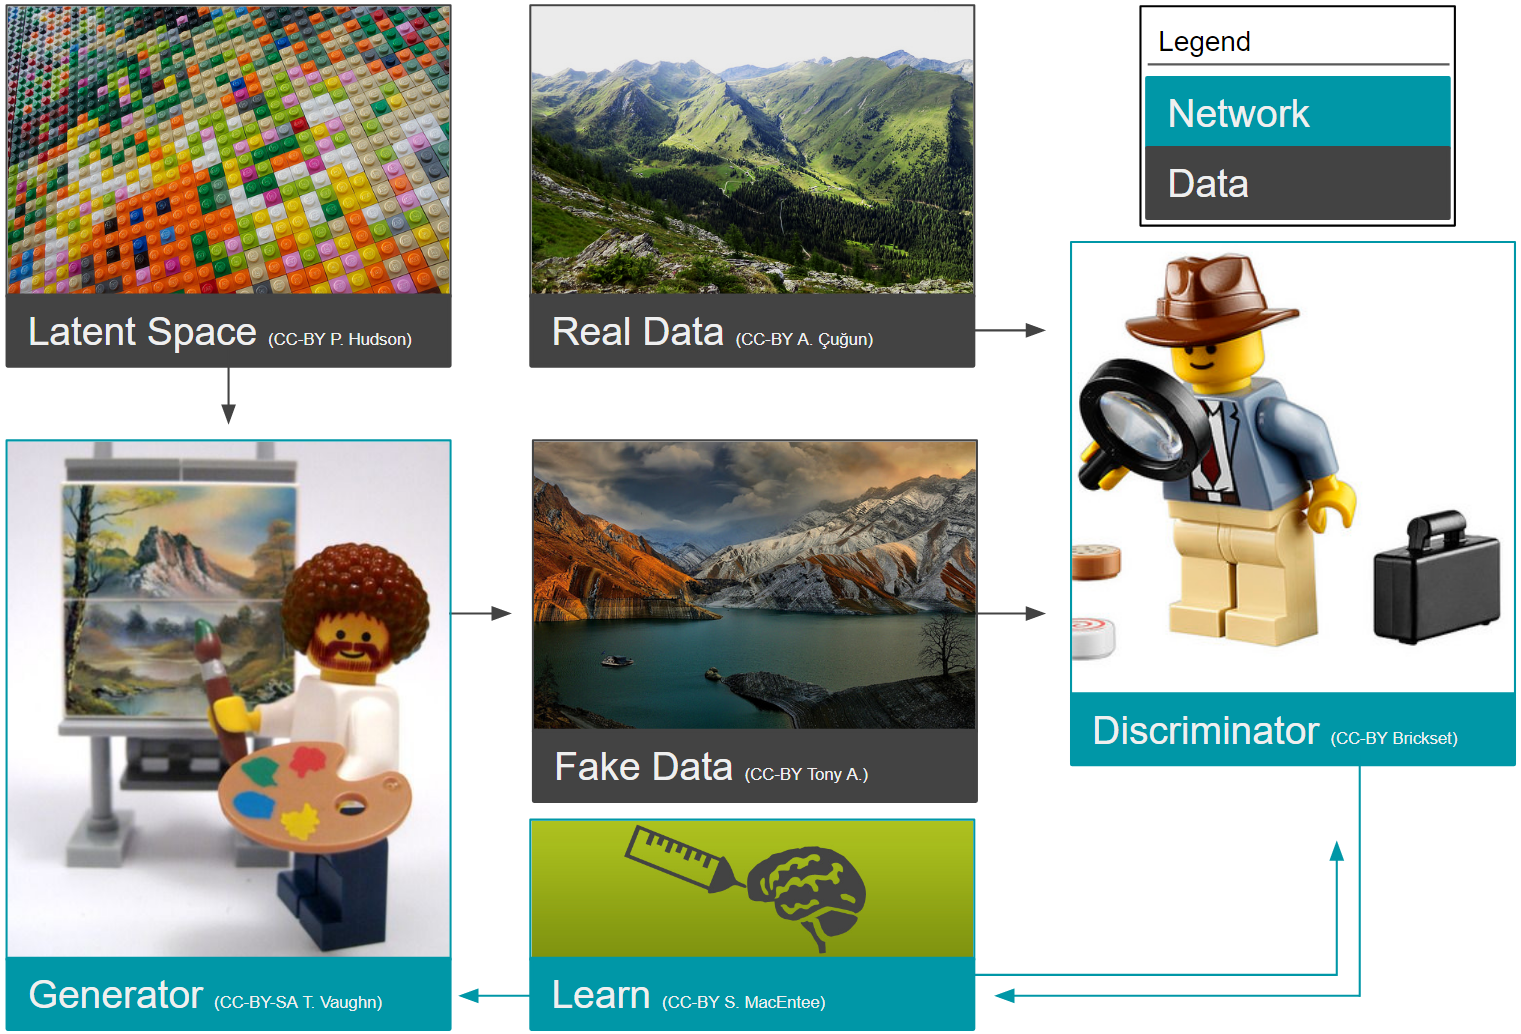
\includegraphics[width=\textwidth]{figures/GAN.PNG}
    \caption{Schematic of a \acl{gan}}
    \label{fig:gan}
\end{figure}

\cref{fig:gan} shows the basic working of \acp{gan}. The arrows are colored in blue and grey, where the blue paths show network feedback and grey shows the progression of data. These networks learn from each other, where the generator draws from latent space (a noise vector) to create a fake version of a target. The discriminator tries to discern whether the presented data is real or generated from the adversarial generator. These networks leverage game theory to outperform each other and comparative networks. They reach a Nash equilibrium during training, which describes the concept on a non-cooperative game reaching steady state \citep{nash1951non}. 

% Considerations for Neural Architectures
\subsection{Neural Architectures}
\aclp{nn} can generally be assembled in different architectures. In \cref{fig:cnnsota} we present reported performances of neural architectures on the classification task of the ImageNet challenge. The colors in this figure express different classes of architectures. Early networks that broke ground as the new \aclp{sota} in image classification are the AlexNet, VGG-16, and VGG-19. These networks clearly do not leverage some tricks that modern CNNs implement, the VGG-16 with a relatively high amount of parameters is known to generalize well on transfer learning tasks however \citep{dramsch2018deep}. 

\begin{figure}[H]
    \centering
    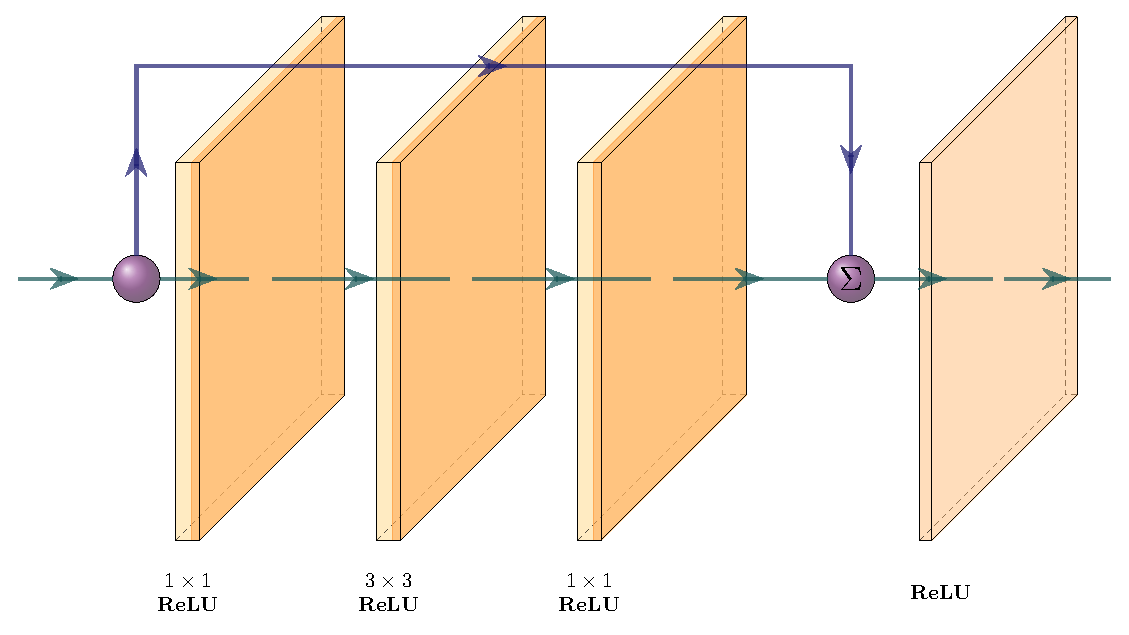
\includegraphics[width=\textwidth,height=5cm,keepaspectratio]{figures/resnet.pdf}
    \caption{Resnet Block with two $1\times1$ convolutional layers that frame a $3\times3$ convolutional layer with \ac{relu} activation each. The result being added with the original data, also known as identity.}
    \label{fig:resnet}
\end{figure}

Research into deep convolutional networks showed that the data in the network would lose signal with increasing depth. Hence, the limitation of VGG at 19 layers. Residual blocks introduced a solution to this problem by implementing a shortcut between the original data and the output from the block. \cref{fig:resnet} presents the original ResNet block architecture, which was used in ResNet-50 and ResNet-101 in \cref{fig:cnnsota} \citep{he2016deep}. Details on ResNet blocks differ, the main take-away being the sum or concatenation of the original data with the block output. DenseNets \citep{huang2017densely} and Inception-style networks \citep{szegedy2015going} are other approaches to build deeper \acp{nn}.

The categories of AmoebaNet, NASNet, and EfficientNet are a more recent development in neural architecture research, based on \acf{nas}. The AmoebaNet is based on Evolutionary Computing and hand-tuning the solution to search for an ideal neural architecture to solve the task \citep{real2019regularized}. The NASNet fixes the overall architecture, but uses a controler \ac{rnn} to modify the blocks within the architecture \citep{zoph2018learning}. The EfficientNet architecture was also acquired by \ac{nas}, by optimizing for both accuracy and FLOPS to reduce the computational cost \citep{tan2019efficientnet}. Moreover, \citet{tan2019efficientnet} derives a method of compound scaling for deep neural networks. While ResNet-50 and ResNet-101 differ only in depth, the authors derive a relationship between depth, width and resolution-scaling of deep neural networks.

\begin{figure}[H]
    \centering
    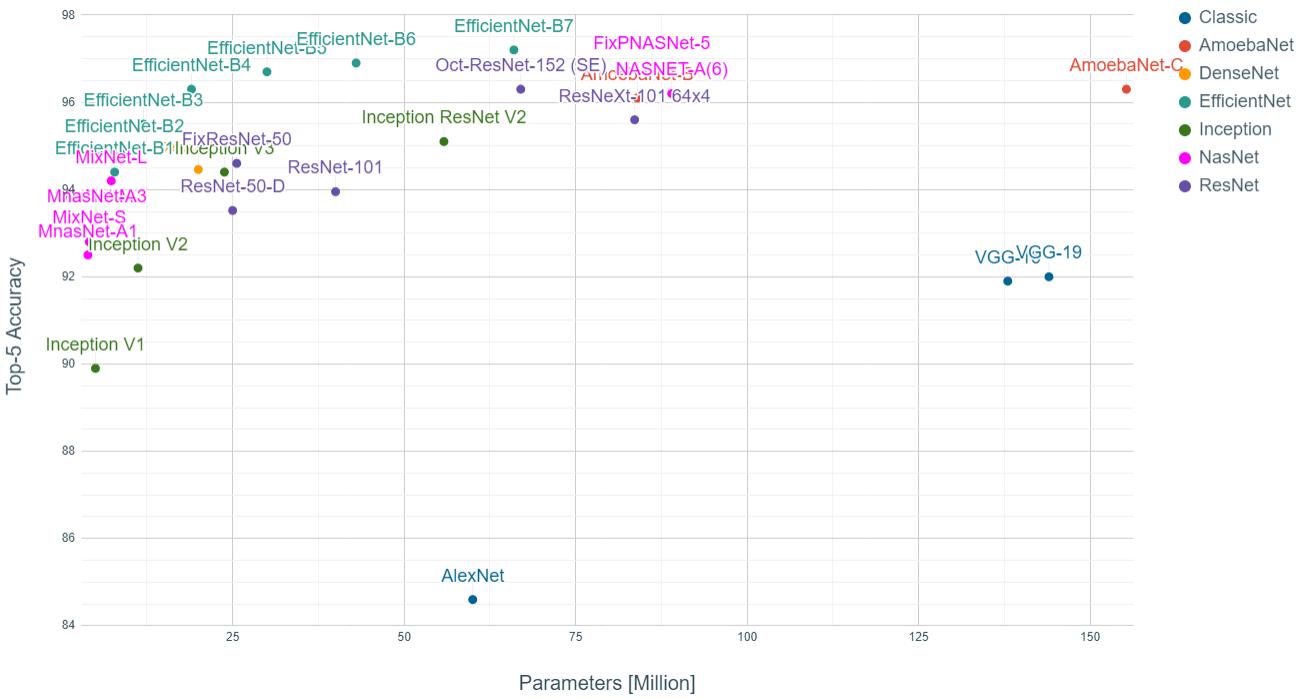
\includegraphics[width=1.1\textwidth]{figures/imagenetsota.png}
    \caption{Top-5 Accuracies of Neural Architectures on ImageNet plotted against Million Parameters, color-coded to similar network type. Data and references shown in \cref{tab:imagenet-sota}}
    \label{fig:cnnsota}
\end{figure}

Apart from building deeper networks for image classification, the neural architectures can serve as a  forcing function to the task the network is built for. Encoder-Decoder networks will compress the data with a combination of downsampling layers, which in the case of a computer vision could either be strided convolutions or pooling layers after convolutional layers. During these operations, the number of filters increases, while the spatial extent is diminished significantly. This encoding operation is equivalent to a lossy compression, with the low-dimensional layer called "code" or "bottleneck". The bottleneck is then upsampled by either strided transpose Convolutions or upsampling layers that perform a specified interpolation. This is the Decoder of the Encoder-Decoder pair. These networks can be used for data compresssion in \acp{ae}, where the decoder restores the original data as good as possible \citep{hinton2006reducing}. Alternatively, the Decoder can learn a dense classification task like semantic segmentation or seismic interpretation.

U-Nets present a special type of encoder-decoder networks, that learn semantic segmentation on from small datasets \citep{ronneberger2015unet}. They form a special kind of \ac{fcn} shown in \cref{fig:unet}. Originally developed on biomedical images, the network found wide acceptance in label sparse disciplines. The Unet implements shortcut connections between convolutional layers of equal extent in the Encoder and Decoder networks. This alleviates the pressure of the network learning and reconstructing the output data from the bottleneck in isolation. 

\begin{figure}[H]
    \centering
    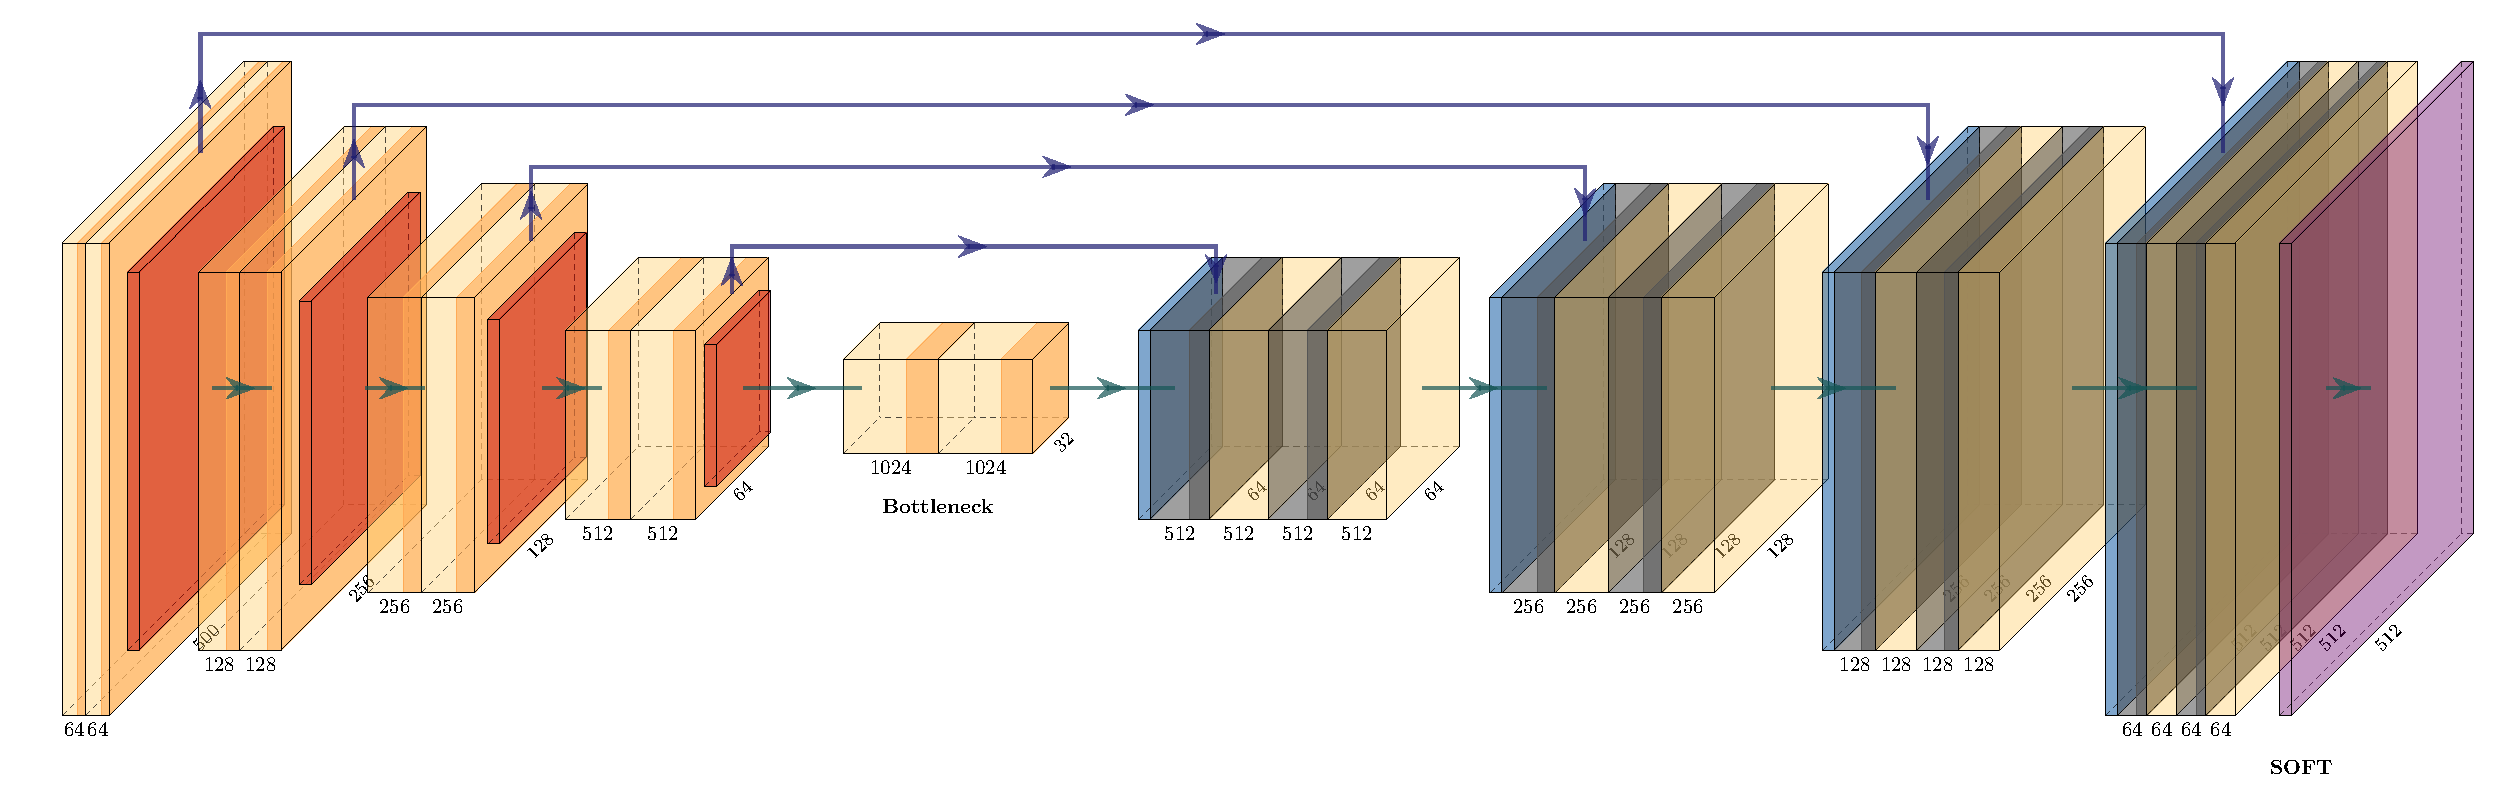
\includegraphics[width=\textwidth,height=5cm,keepaspectratio]{figures/unet.pdf}
    \caption{Unet after \citet{ronneberger2015unet} using 2D convolutional layers (yellow) with \ac{relu} activation (orange) and skip connection between equal-dimensional layers. The Encoder uses pooling (red), while the Decoder uses Upsampling layers (blue), witha final SoftMax layer (purple) for classification / semantic segmentation}
    \label{fig:unet}
\end{figure}

\section{Machine Learning in Geoscience}
The development of the subfield of deep learning has lead to advances in many scientific fields that are not directly related to the larger field of artificial intelligence. This section focuses on historic use-cases of machine learning models in geoscience and evaluate these in the context of recent advances in deep learning. I provide an overview of supervised and unsupervised methods that have persevered. Furthermore, I distinguish implementations of deep neural network topologies and advanced machine learning methods in geoscientific applications. I go on to investigate where these methods differ from previously unsuccessful attempts at application.

Early on \acf{ml} has been reviewed in a geophysical context. Early publications of \ac{ml} in geoscience apply \acp{nn} to geophysical problems. Particularly seismic processing lends itself to explore \acp{nn} as general functional approximator \citep{Hornik1989-bl}. \citet{McCormack1991-pm} review of the emerging tool of neural networks in 1991. He highlights the application of pattern recognition and is very succinct in describing basic math associated with neural computing. The wording of most parts has changed, as compared to today. Generally this gives a good baseline and McCormack gives a good illustration and overview with examples in well log classification and trace editing. As the paper appeared in The Leading Edge, it is not peer reviewed, yet it does give a good historic overview. The author summarizes \ac{nn} applications over the 30 year prior to the review and hightlights automated well-log analysis and seismic trace editing. The review comes to a conclusion that these methods show promise as general approximators. 

\citet{Van_der_Baan2000-jz} review the most recent advancements in \acfp{nn} in geophysical applications. It goes into much detail on the neural networks employed in 2000 and the difficulties in building these models and training them. They identify the following subsurface geoscience applications through history: First-break picking, electromagnetics, magnetotellurics, seismic inversion, shear-wave splitting, well log analysis, trace editing, seismic deconvolution, and event classification. The authors evaluate the application of \acp{nn} as subpar to physics-based approaches. The paper concludes that neural networks are too expensive and complex to be of real value in geoscience. Generally, this review focuses very much on exploration geoscienc. 

\citet{Mjolsness2001-fq} review \ac{ml} in a broader context outside of exploration geoscience. They illustrate recent successes of \ac{ml} in analyzing sattelite data and computer robotic geology. The authors include graphical models, \acp{rmm}, \acp{hmm}, and \acp{svm}. They further highlight limitations to vector data, therefore failing richer data such as graphs and text data. Moreover, the authors from NASA JPL go into detail on pattern recognition in automated rovers to identify geological prospects on Mars. They state:
\begin{quote}
“The scientific need for geological feature catalogs has led to multiyear human surveys of Mars orbital imagery yielding tens of thousands of cataloged, characterized features including impact craters, faults, and ridges.” - \citep{Mjolsness2001-fq}
\end{quote}
The authors evaluate how especially the introduction of \ac{svm} have allowed the identification of geomorphological features without modeling the processes behind. Further they mention recurrent neural networks in gene expression data, a method that has experienced a renaissance in deep learning. The paper is very short and succinct in evaluating prospects without going into detail on the algorithms itself. In contrast, we expect our review to go more into depth and explore the applications in geoscience further.

\subsection{History of Machine Learning in Geoscience}
Machine learning, statistical, and mathematical models have a long history in geoscience. Markov models have been used to describe sedimentology as early as the 1970s \citep{schwarzacher1972semi} and the use of k-means in geoscience as early as 1964 \citep{preston1964fourier}. In geophysics applications of \acp{nn} to perform seismic devonvolution were published in the 1980s \citet{Zhao1988-hu}. Early tree-based methods were chiefly used in economic geology and exploration geophysics for prospectivity mapping with \acfp{dt} \citep{newendorp1976decision,reddy1991decisiontree}. \ac{svm} has early on been applied to AVO classification \cite{Li2004-fk} and geological facies delineation for hydrological analysis \citep{Tartakovsky2004-ml}. Due to some changes in nomenclature of methods through time, it has been difficult to identify all publications. Moreover, this thesis mostly focuses on the application of \acp{nn}, however, we give an additional overview of geoscientific applications of shallow \ac{ml}.

\subsubsection{Neural Networks in Geoscience}
Early applications of neural networks were prominent in seismic data processing and analysis. \citet{Zhao1988-hu} use a \ac{nn} to perform seismic deconvolution early on. An application of seismic inversion with \acp{nn} was published by \citet{Roth1994-na}. Early \ac{ml}-based electromagnetic geophysics performs subsurface localization \citep{Poulton1992-ft} and magnetotelluric inversion via Hopfield \acp{nn} \citep{Zhang1997-yp}. \citet{Feng1998-ck} applied \ac{nn} to model geomechanical microfractures in triaxial compression tests. Interestingly, \citet{Legget1996-nk} used a combination of \acf{som} and back-propagation \acp{nn} that function similar to modern day \acfp{cnn} to perform 3D horizon tracking \citep{Leggett2003-vq}. With the recent \ac{dl} explosion, papers on seismic interpretation have gotten very popular, given the similarity to 2D segmentation tasks (cf. \cref{tab:geonn}).

\begin{table}[]
    \centering
    \begin{tabularx}{\textwidth}{l|X}
\toprule
Topic & Publications \\
\bottomrule
\toprule
First Break Picking & \citet{Murat1992-qs, McCormack1993-ul, Dai1997-ta, Ross2018-kt} \\
\midrule
Ground Penetrating Radar & \citet{Al-Nuaimy2000-sa, Gamba2000-va, Shihab2002-po, Shihab2002-ne, Youn2002-rn, Birkenfeld2010-rd, Cui2010-rn, Maas2013-wb, Nunez-Nieto2014-il, Mertens2016-os, Hansen2017-rq, Kilic2018-to}\\
\midrule
Seismic Deconvolution &  \citet{Zhao1988-hu, Wang1997-is, CalderonMacias1997-pl, Harrigan1991-ij}\\
\midrule
Seismic Horizon Picking & \citet{Huang1990-hj, Legget1996-nk, Zhang2001-hy, Leggett2003-vq}\\
\midrule
Seismic Interpretation & \citet{Meldahl2001-bb, Strecker2002-dp, Klose2006-xh, Zheng2014-il, Marroquin2014-gg, Qi2016-qy, Zhao2016-ya, Roden2015-ek,Huang2017-fk, Lewis2017-ek, Waldeland2017-tx, Guo2017-ij, Zhao2017-gv, Veillard2018-sg, Araya-Polo2017-ky,dramsch2018deep, Chevitarese2018-kd, Gramstad2018-ql, Guitton2018-gd, Purves2018-dy, Shafiq2018-qt, Shafiq2018-ed, Waldeland2018-hj, AlRegib2018-yr, Le_Bouteiller2018-ma, Li2018-bm, Sacrey2018-pk, Shafiq2018-rp, Wu2018-hg}\\
\midrule 
Seismic Inversion & \citet{Roth1994-na, Langer1996-fv, Iturraran-Viveros2012-ta, Ansari2014-ci, Verma2014-jx, Golsanami2015-ul, Schuster2018-sj, Araya-Polo2018-xf, Mosser2018-nf, Mosser2018-hm, Richardson2018-py}\\
\midrule
Seismic Tomography & \citet{Bauer2008-pv, Braeuer2015-yj}\\
\midrule
Seismic Well-Tie & \citet{Chaki2018-mr}\\
\midrule
Well-Log analysis & \citet{Huang1996-eg, Fung1997-kw, Bhatt2002-kj, Helle2002-ju, Asoodeh2014-mm, Anifowose2017-bx, Saporetti2018-sq, Maiti2010-dw, Chang2002-oi, Bauer2015-hy, Emelyanova2017-vy, Carreira2018-bp}\\
\bottomrule
\end{tabularx}
    \caption{Neural Networks in Geophysics}
    \label{tab:geonn}
\end{table}

\subsection{Challenges of machine learning in geoscience}
Statistical methods and machine learning are based on several assumptions and demand some pre-requisites that can cause problems in geoscience. These include the assumption that data is \acf{iid} and the pre-requisite of a ground truth for supervised learning. In this section I discuss these challenges and present some approaches to solve these problems.

% Inherent properties of data
% Talk about IID in geoscience
% imbalanced data
% heterogeneities in geoscience and ml - > distributions

Geoscientific data is known to be very heterogeneous across vastly different scales (mm to km), which makes the system hard to model in general. Additionaly, a core assumption of statistics \ac{iid} is usually in conflict with the geological processes. Regionality of depositional patterns violates the assumption data is identically distributed and time-dependent processes, such as systems tracts in sedimentology, violate the independence assumption of individual samples. This fact has to be taken into account, when choosing models and sampling methods. Expanding on the sedimentology example, the time-varying deposition can be modelled as markovian \citep{schwarzacher1972semi}, instead of treating samples as strictly independent. Moreover, sampling of any data needs to honour the clustering in distribution of samples. Stratified sampling \citep{kish1965survey} can alleviate sampling bias. Additionally, stratified sampling can address the problem that geoscientific data often contains imbalanced data. Imbalanced data implies that the number of samples per class in the label data set is not uniformly distributed. These imbalances can stem from the fact that different depositional regimes cause different thicknesses in the stratigraphic columns, for example commonly leaving thicker sand columns and fine shale layers. Alternatively, imbalances can stem from the data collection process itself, be it that seismic data does not adequately image variations below 1~m or the location where data is collected, considering that e.g. hydrocarbon companies do not choose the location for 3D seismic data acquisition randomly. This imbalance due to non-uniform sampling can not be solved by sampling itself, as the bias is implicit in the available data itself. 

% measurements and data
% availability of data
% Talk about no ground truth


In the computer vision community hand-labelled data sets like ImageNet, CIFAR, and PASCAL-VOC are openly available, which catalyzed the developed new architectures and approaches in deep learning. Geoscientific data is often expensive to acquire and companies are reluctant to make data available, less even for processed or interpreted data. Early machine learning workshops often showed results on the open Dutch F3 dataset, however, national data repositories have started to change this approach to foster innovation. With data becoming more available, the next problem is the lack of ground truth. Obtaining accurate labels for seismic data is impossible, as any inversion process is non-unique and digging is not practical. In other imaging-based fields (e.g. radiology) that rely on interpretation of imaging results, studies investigate both interinterpreter variations, by making several interpretations available and intra-interpreter variability by re-interpreting the dataset after a set time interval \citep{macerlean2013, alikhassi2018comparison,al2010inter}. Additionally, simulations provide a ground truth, but can implicitly include modelling assumptions in the data or commit the inverse crime \citep{wirgin2004inverse}. The inverse crime presents the problem of modelling and inverting data with the same theoretical ingredients.

% Talk about metrics
% Seismic dynamic range (clip = .97)
% noise

In geophysics itself, seismic data presents a unique challenge to computer vision problems, in that the \~3\textsuperscript{rd} percentile of amplitudes occupy large parts of the dynamic range. Displays of seismic data usually clip amplitudes to make most of the seismic amplitude content visible, this has also proven to be a viable preprocessing step before feeding seismic data to computer vision systems, such as convolutional neural networks. Machine learning systems have been known to be vulnerable to noise. This noise can be physical noise (i.e. low SNR) for simpler models or adversarial attacks that reverse engineer more complex models to fool said model. Adversarial attacks include a one-pixel attack on ImageNet classifiers \citep{su2019one}, humanly imperceptible noise \citep{goodfellow2014explaining}, or physical stickers \citep{brown2017adversarial}. In addition, geological data contains regions of geological interest and regions that are inconsequential, this has not been represented in metrics adequately \citep{purves2019towards}.

% solutions?
% talk about transfer learning (myth of big data)
% Self-supervision
% multi+task learning

Realistically, the sparsity of labelled ground truth data can be addressed in different ways. In the case when labels are available but not abundant, transfer learning of highly generalizable models like VGG-16 can be fine-tuned to seismic data. The VGG-16 architecture can also be included in U-Nets as a decoder to leverage the benefits of transfer learning in semantic segmentation tasks \citep{dramsch2018deep}. Moreover, weakly-supervised training can preform label propagation of labeled sections of the full data set to unlabeled sets. Unsupervised or self-supvervised training can be applicable, where no reliable ground truth is available, but a desired operation on the data is known or an internal structure of the data can be exploited \citep{dramsch20193dwarping}. Additionally, multi-task learning has been shown to be able to stabilize network performance in \acl{nlp} \citep{liu2019multi} and \acl{rl} \citep{yu2019meta}.

% explainability and complexity

One caveat of increasingly performant but complex machine learning models is stakeholder buy-in or trust. These issues can be adressed, by benchmarking complex models against simpler models and physics-based solutions. Additionally, model explainability has become an important topic of research \citep{NIPS2017_7062}. \citet{ribeiro2016should} introduce the \acf{lime} method to gain insight into black-box models for individual samples. \citet{shrikumar2017learning} propose a method to propagate activations in \aclp{dnn}. The Grad-CAM algorithm \citep{selvaraju2017grad} provides attention-like explanations for \acp{cnn} in computer vision tasks, to explain the main contributors to a classification output. Additionally, strict adherence to train-val-test splits and exploration of biases within the data can be essential. 





%!TEX root = ../Thesis.tex
\chapter{Synopsis}
\label{sec:synopsis}
The following chapters are comprised of four journal papers that are supplemented with two conference papers and four workshop papers, of which all are peer-reviewed or submitted to peer-reviewed journals. I combine several papers into topical chapters for conciseness. This thesis follows a data science workflow, starting with exploratory data analysis to gain insight to the specific geology and field. I go on to present groundwork on machine learning and data processing on 4D seismic data. Based on this groundwork, I developed a method for 4D seismic inversion a novel unsupervised 3D time-shift extraction method for 4D seismic. This chapter summarizes these papers and places them in the appropriate context for the thesis.

%!TEX root = ../Thesis.tex
\section{Data Preparation}
% aabo2017correlation
% aabo2018integrated
% dramsch2018gaussian

In \cref{sec:dataprep} I include one published journal paper \citep{aabo2018integrated}, one published conference paper \citep{aabo2017correlation}, and one published workshop paper \citep{dramsch2018gaussian}. The published conference paper with the title \citetitle{aabo2017correlation} contains preliminary work contributing to and extended in the journal paper \citetitle{aabo2018integrated}. Whereas, the workshop paper with the title \citetitle{dramsch2018gaussian} is an independent study of backscatter scanning-electron microscopy data on chalk thin slices.

The data for this thesis was acquired in the Danish North Sea. The main hydrocarbon reservoirs in the Danish Central Graben area consist of chalk, a sedimentologically distinct feature in the seismic data. The chalk layer is high in porosity (20-35\%), however, very low in permeability 3~mD to less than 1~mD. In \citet{aabo2017correlation} we presented an integrated fracture study of the Ekofisk chalk Kraka field in the South Central Graben. Within this preliminary study, we performed a localized fracture study along one well-bore to compare fracture measurements from core, well logs and seismic data. Initial analysis of the seismic data showed a maximum vertical resolution of \~40~m, which did not yield sufficient results for comparative study. 
% These data were prepared individually by three researchers, with my contribution being the analysis and preparation of the seismic dataset. 

\begin{figure}[!ht]
    \centering
    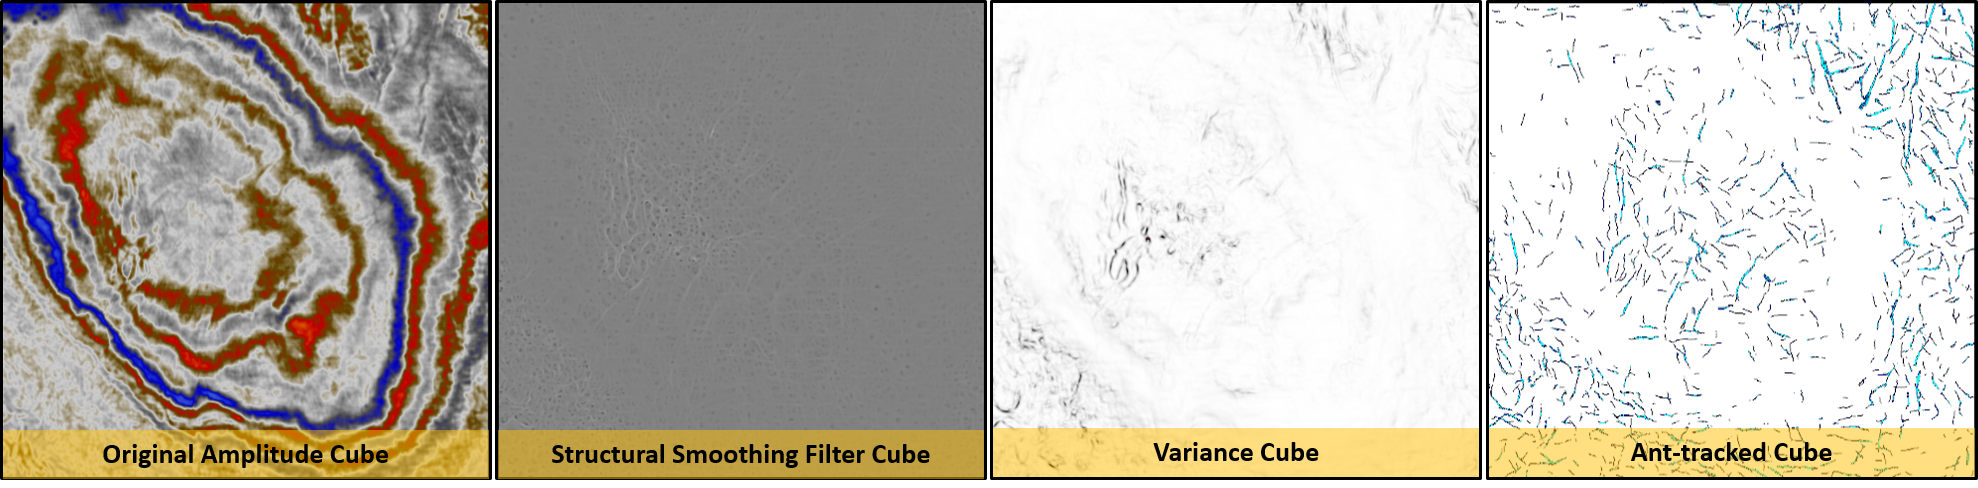
\includegraphics[width=\textwidth]{figures/seismic-comparisons.png}
    \caption{Comparison of seismic data, structural smoothed, variance and ant-track time slice}
    \label{fig:seismic-comparison}
\end{figure}

\cref{fig:seismic-comparison} contains several post-stack seismic attributes to enhance lineaments within the seismic cubes. While the variance and structural cubes yielded some initial promise the following image processing workflow yielded the best results. These were geared towards enhancing vertically coherent structures. This was achieved by a workflow including colorspace transformations and ant-tracking, which is a search algorithm leveraging biologically inspired software agents.

Normally, images are shown in \ac{rgb} colorspace, however, these can be transformed into other space, such as, \ac{cmyk} and \ac{hsv}. The \ac{hsv} colorspace is commonly used in image analysis to detect edges on the gradient of the saturation values. Therefore, it serves as a good target colorspace for image processing. To achieve this, the bit-depth of seismic data has to be increased, considering that natural images displayed on modern monitors contain \~32 million colors with a bit-depth of 24~bit for color representation.
This is achieved by replicating the seismic cubes with a static timeshift to create an \ac{rgb} representation \citep{laake2014structural}. In our case a small shift below 3~ms to avoid loss of small-scale fractures and avoid smearing yielded the best results. 

Consequently, after a colorspace transformation to \ac{hsv}, the biologically inspired ant-track algorithm was applied to the saturation gradient volume. The ant-tracking algorithm implements unsupervised software-agents that search the vicinity in a 3D volume to find spatially coherent features \citep{dorigo1992optimization}. The software agents can be instructed to be more or less aggressive in their search, where I chose a moderate setting, which will enhance faults well but maintains nuance of the faults. The workflow for fault extraction is shown in \cref{fig:seismic-workflow}.

\begin{figure}[!ht]
    \centering
    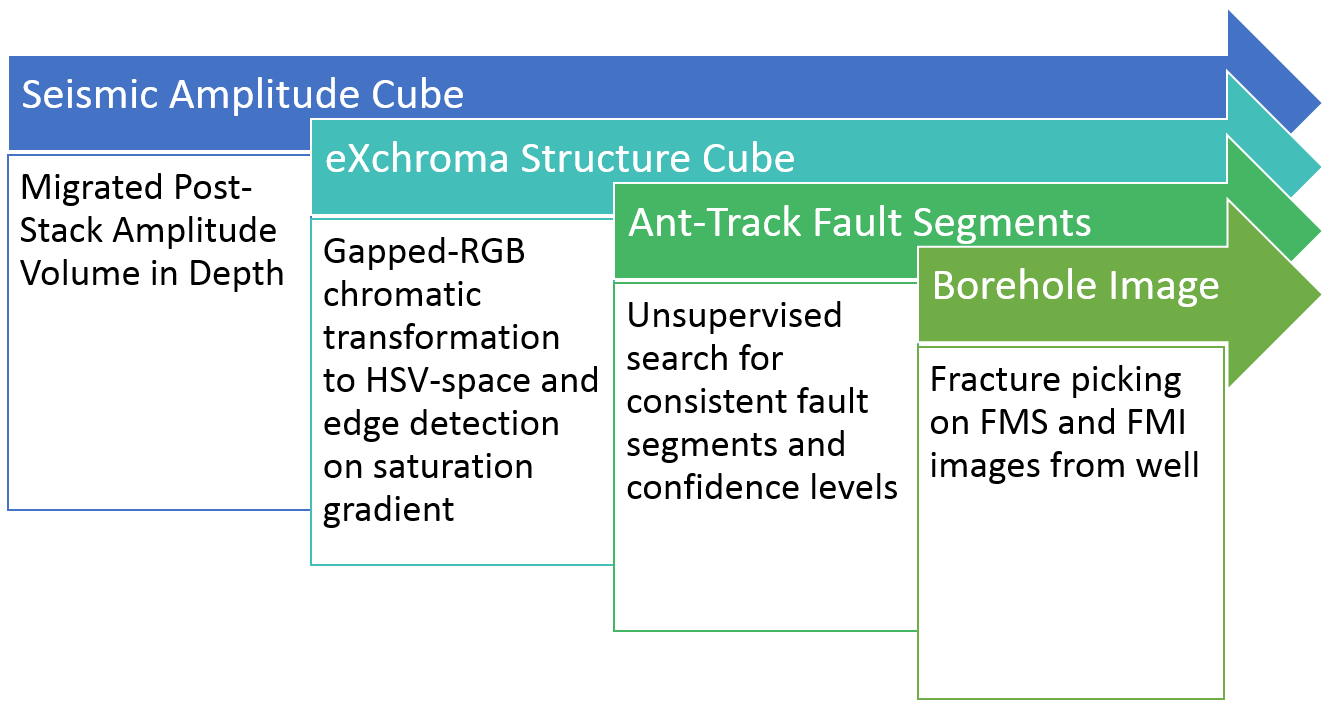
\includegraphics[width=\textwidth]{figures/fracture-workflow.PNG}
    \caption{Workflow to identify fractures in post-stack seismic data to prepare for comparison to borehole analysis}
    \label{fig:seismic-workflow}
\end{figure}

A joint interpretation of the seismic and ant-track volumes yielded a focused seismic interpretation along the well-bore, where \acf{bhi} data were available for comparison (after the interpretation to avoid bias). These match the independent interpretation of the well data closely in orientation and distribution of fractures. It is likely that these represent fracture corridors, small faults or damage zones in the chalk. This preliminary study was able to show that seismic provides a valuable method for mapping the size, orientation and connectivity of fracture zones away from the well. 

Following this initial study, the seismic interpretation was extended for to regional fault systems and \ac{bhi} to several wells for \citet{aabo2018integrated} presented in \cref{sec:tala}. The analysis of ant-tracked attribute volumes, allowed us to relate structural trends below the resolution of amplitude seismic to features at different scales. This interpretation suggests that the fracture pattern is more complex than previously suggested. We propose that fracture generation and propagation in the field is in part controlled by the regional maximum horizontal stress from the seismic interpretation in addition to the halokinesis in the South Central Graben. 

The seismic analysis was correlated with the fracture analysis from \ac{bhi} data and core analysis in multiple wells. The fracture analysis was particularly dependent on the Terzaghi-correction \citep{terzaghi1965sources} to obtain the in-situ fracture orientation. This work identified two main fracture trends in the Danian Ekofisk reservoir. The main fracture set strikes sub-parallel to the regional NE/NNE maximum horizontal stress present on all horizontal/deviated wellbores and core. The vertical fracture distribution of the Kraka Field studied in a single well, due to availability. Within this single well the NE/NNE fracture distribution was continuous. This main NNE/NE fracture trend was traced from well scale to ant-tracked scale bridgeing the scale-gap. Regional large-scale faults interpreted on the raw amplitude seismic are present in the ant-tracked cube, trending NE, which indicates that the NNE trend is representative for smaller-scale lineations, with a Northern deviation on regional scales. 

Further research into the porosity and sedimentology of the chalk reservoirs conducted on microscoping scales focused on identifying porosity using \acf{bsem} in \cref{section:gaussian}, which comprises the third paper in this chapter \citep{dramsch2018gaussian}. Identifying the grain size and orientation of the oolites is usually a manual work-intensive task, ideal for computer vision tasks, considering the good contrast of light-grey to white oolites and the black background. Unfortunately, training data was not available, which led me to experiment with unsupervised clustering to find the ideal boundary of the grain. Gaussian Mixture Models learnt a two-fold representation that separated the background well from the rock. Any single-valued decision boundary will be non-smooth, which can be alleviated by morphological filtering. Smooth boundaries are essential for chalk grains, as geologists are interested in the perimeter of the oolites to calculate the specific surface. The optimal boundary of chalk grains could then be used to generate training data for more sophisticated machine learning systems.

% This chapter enabled me to explore the Danish North Sea data in Kraka, Dan and Halfdan, as well as, implement data science principles on geological problems. Collaborating with geologists on these papers resulted in a better understanding of underlying processes in the chalk and 4D effects of production, due to compaction, stimulation and chalk weakening. The seismic analysis improved my understanding of the geological structures and trendlines in the South Central Graben area, while contributing to an improved understand of the scale-dependence of the stress fields and a method capable of extracting an optimal boundary of chalk in \ac{bsem}. 

In the first study of this chapter \citep{aabo2017correlation} I applied an image processing workflow to enhance the vertical resolution of seismic data. Consequently, I could transform the data to introduce a biologically inspired software algorithm to enhance and identify lineaments for interpretation. This work was essential in enabling a localized pilot study to relate localized features from well-scale \ac{bhi} to enhanced seismic-scale, verifying the seismic image analysis. This pilot study fed into a larger study \citep{aabo2018integrated}, where a fracture study from core and \ac{bhi} was related to both the enhanced ant-tracked volume and a regional fault interpretation, updating the understanding of the fracture generation in the Salt Dome Process in the Danish South Central Graben area. The third study solved a manual process using an unsupervised image analysis tool paired with strong data science principles, providing a novel reliable tool to geologists in \ac{bsem} analysis.

%!TEX root = ../Thesis.tex
\section{Foundational Research}

The foundational research in this thesis includes publications on \acl{dl} and 4D seismic in \cref{sec:foundations}. These publications apply a signal processing-approach to both 4D seismic and \acl{ml}. I include a paper that takes a tutorial-view of dynamic time-warping a 4D seismic time shift analysis tool and introduces a novel constraint to improve performance of the algorithm. I then go on to present a possible source of misclassification in neural networks on non-stationary physical data such as seismics. I further investigate a possible solution to the aliasing problem of \aclp{cnn} for seismic, including complex-valued operations withing the network. I further investigate the assumption that massive interpreted datasets have to be available for successful training of \aclp{dnn} and present a working solution for smaller datasets.

\begin{figure}[!hb]
    \subbottom[\citet{Itakura1975} Parallelogram]{%
     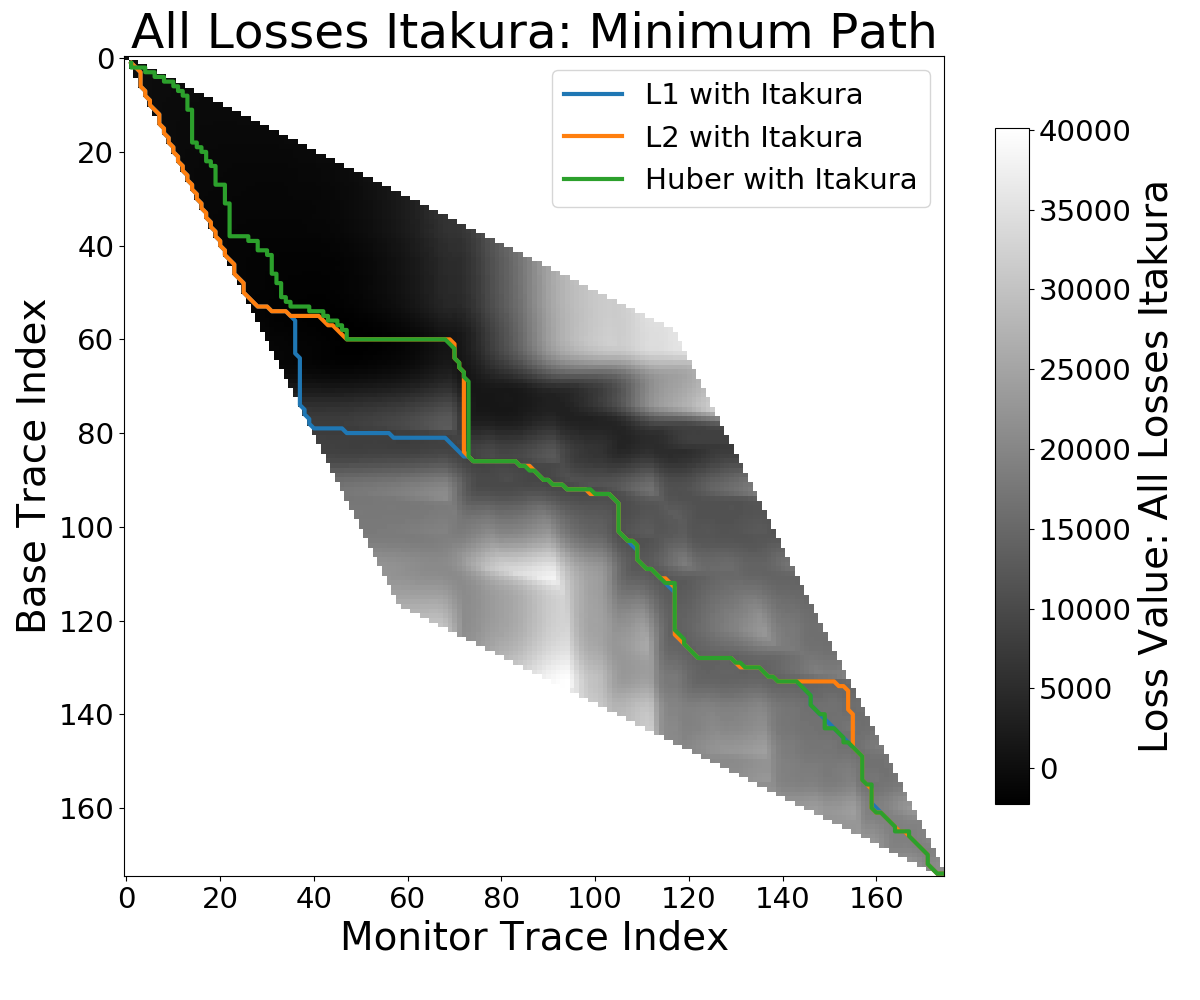
\includegraphics[width=.3\textwidth]{figures/minimum_path_all_losses_itakura_.png} \label{fig:itakura}
    }
    ~
    \subbottom[\citet{Sakoe1978} Disc]{%
     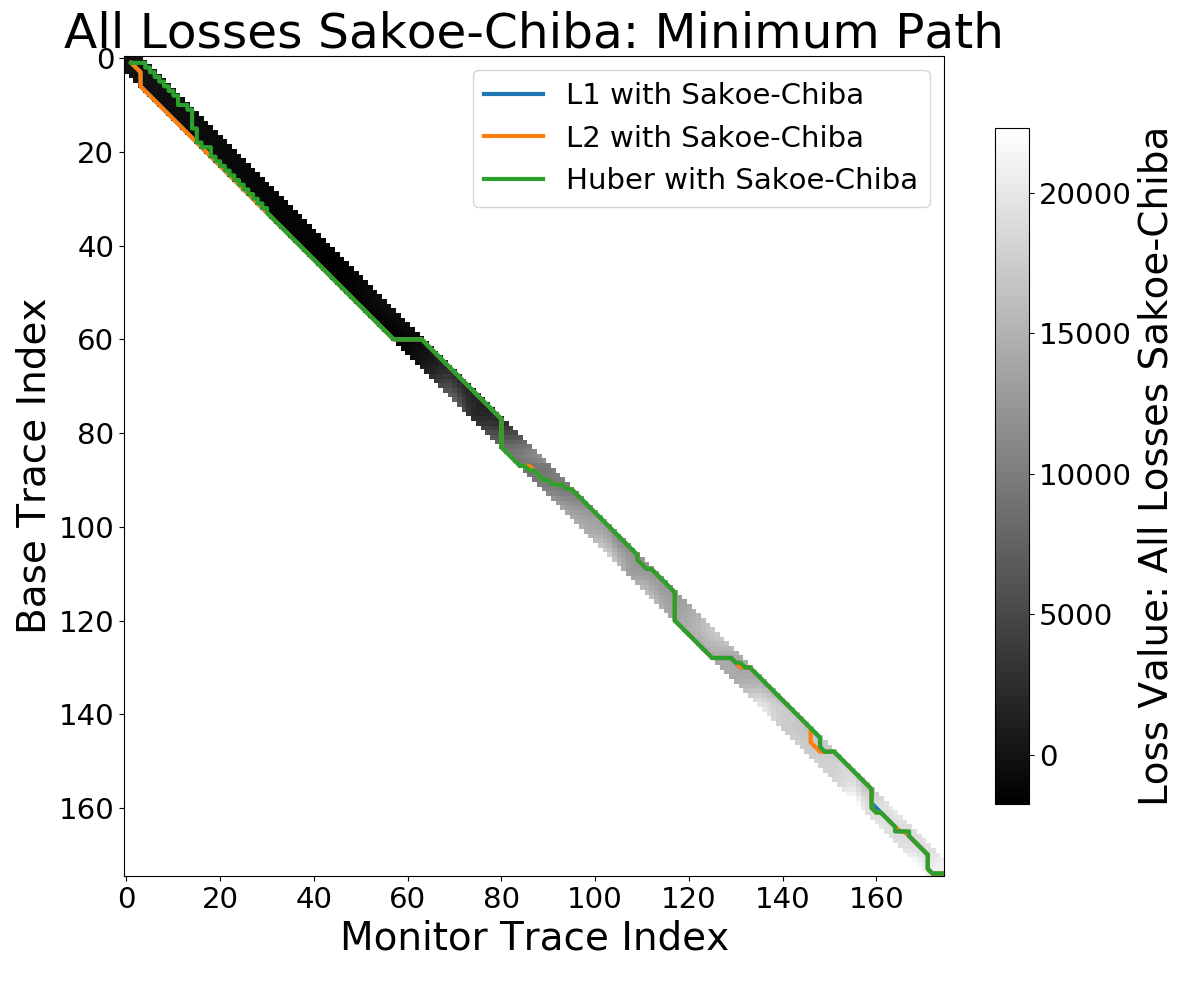
\includegraphics[width=.3\textwidth]{figures/minimum_path_all_losses_sakoe_chiba_.png} \label{fig:sakoe}
    }
    ~
    \subbottom[LB\_Envelope \citep{keogh2005exact}]{%
     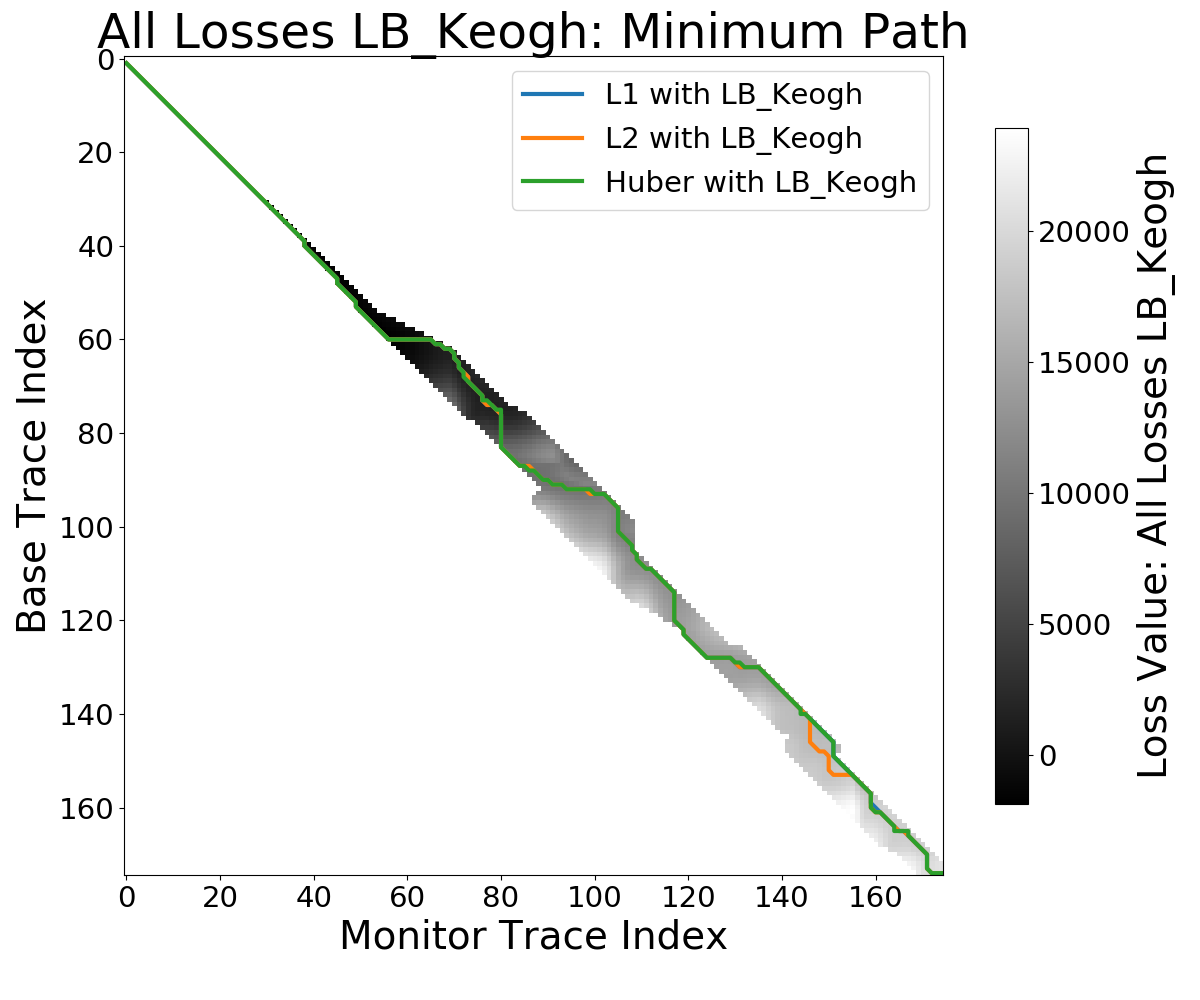
\includegraphics[width=.3\textwidth]{figures/minimum_path_all_losses_lb_keogh_.png}\label{fig:lbk}
    }
\caption{Minimum path for constraint masks for cumulative cost in \ac{dtw}. Images show the optimum path for different loss functions $L_1$, $L_2$, and Huber loss \citep[from][]{dramsch2019dtw}}
\label{fig:constraints}
\end{figure} 
% dramsch2019dtw
\citet{dramsch2019dtw} presents a tutorial of \acf{dtw}. \ac{dtw} is a powerful signal processing tool introduced to 4D seismic analysis by \citep{Hale2013} on synthetic data. 4D seismic data relies on alignment of the seismic volumes. This enables interpreters to compare the amplitudes differences of the data. Due to the capability of \ac{dtw} to match arbitrary time-series, it is applicable to 4D time shifts, seismic-well ties, well-to-well ties, and seismic pre- and post-stack migration \citep{Luo*2014}.  \ac{dtw} is known to be computationally slow and expensive, while extracting poor matches on seismic field data. This tutorial paper goes into detail of the \ac{dtw} algorithm, exploring similarity measures, optimization, and constraints interactively through reproducible implementation in Python.

\begin{algorithm}
\begin{algorithmic}
\Procedure{DTW}{$a,b$}
\State Given: Trace $a$ and Trace $b$ of lengths $n$.
\Function{Calculate distance matrix $D$}{$a,b$}
    \State $D \gets dist(a,b)$
\EndFunction
\Function{Calculate Cumulative Cost $C$}{$D$}
\State $C[0,0] \gets 0$
\For {$i = 1$ to $n$} \Comment{Populate Edge}
    \State $C[0,i] \gets D[0,i] + C[0,i-1]$
    \State $C[i,0] \gets D[i,0] + C[i-1,0]$
\EndFor
\For {$i = 1$ to $n$} \Comment{Fill Cumulative Cost Matrix}
    \For {$j = 1$ to $n$} 
        \State $C_{min} \gets \textbf{min} \{C[i,j-1], C[i-1,j-1], C[i-1,j]\}$
        \State $C[i,j] \gets D[i,j] + C_{min}$
    \EndFor
\EndFor
\EndFunction
\Function{Backtrack minimum cost path $P$}{$C$}
\State $P \gets C[n,n]$
\While {$i > 0 | j > 0$}
    \State $i, j \gets \textbf{index} \{ P[last] \}$
    \State $C_{min} \gets \textbf{min} \{C[i,j-1], C[i-1,j-1], C[i-1,j]\}$
    \State $P.\textbf{append} \gets \textbf{index} \{ C_{min} \}$
\EndWhile
\EndFunction
\State \Return {P}
\EndProcedure
\end{algorithmic}
\caption{\acl{dtw} algorithm consists of calculating the element-wise distance matrix, cumulative cost and then find the optimal path in the cumulative cost matrix} \label{dtw}
\end{algorithm}

The \ac{dtw} algorithm, represented in \cref{dtw}, relies on calculating a distance matrix sample-wise between two traces. This is the first avenue of optimization we explore in this paper. The commonly used $L_1$ norm to calculate the distance norm is shown to perform worst out-of-the-box calculating $|b-a|$. Alternatively, the euclidean distance or $L_2$ norm can be used, which modifies the calculation to $(b-a)^2$. The difference between $L_1$ and $L_2$ is significant in the sense that the $L_1$ norm is not differentiable or convex, however it scales linearly for outliers. The $L_2$ norm converges fast close to zero, however the error "explodes" for outliers. We introduce a constraint used in convex optimization, which combines the advantages of the $L_1$ norm and $L_2$ norm, namely the Huber loss:

\begin{equation}
L_\delta (a, b) = 
\begin{cases}
 \frac{1}{2} (b-a)^2 & \text{for } |b-a| \le \delta, \\
 \delta (|b-a| - \frac{1}{2} \delta), & \text{otherwise.}
\end{cases}
\label{eq:huber}
\end{equation}

which is convex for small values, scales linearly for outliers and is differentiable for all values of $\mathbb{R}$, with $\delta$ being a scaling factor.

Additionally, the search space on the cumulative distance matrix can be constrained to both increase performance and avoid non-optimal solutions. The different contraint strategies are presented in \cref{fig:constraints}. The Itakura parallelogram \citep{Itakura1975} in \cref{fig:itakura} describes a parallelogram that that has the largest width agress the diagonal of the matrix, providing the most flexibility for the \ac{dtw} algorithm in the center parts of the seismic traces. The Sakoe-Chiba disc \citep{Sakoe1978} follows a different strategy, which provides a constant maximum warp path. This strategy in \cref{fig:sakoe} introduces a global maximum time shift. Contrary to these two global constraints, we introduce the LB\_Keogh \citep{keogh2005exact} constraint in the paper. This lower bounding method provides a mathematical lower bound for the \ac{dtw} algorithm. We use this lower bound to constrain the warp path, which provides larger variability to high amplitude areas, where cycle-skipping can occur, presented in \cref{fig:lbk}. 

\begin{figure}[!ht]
    \centering
    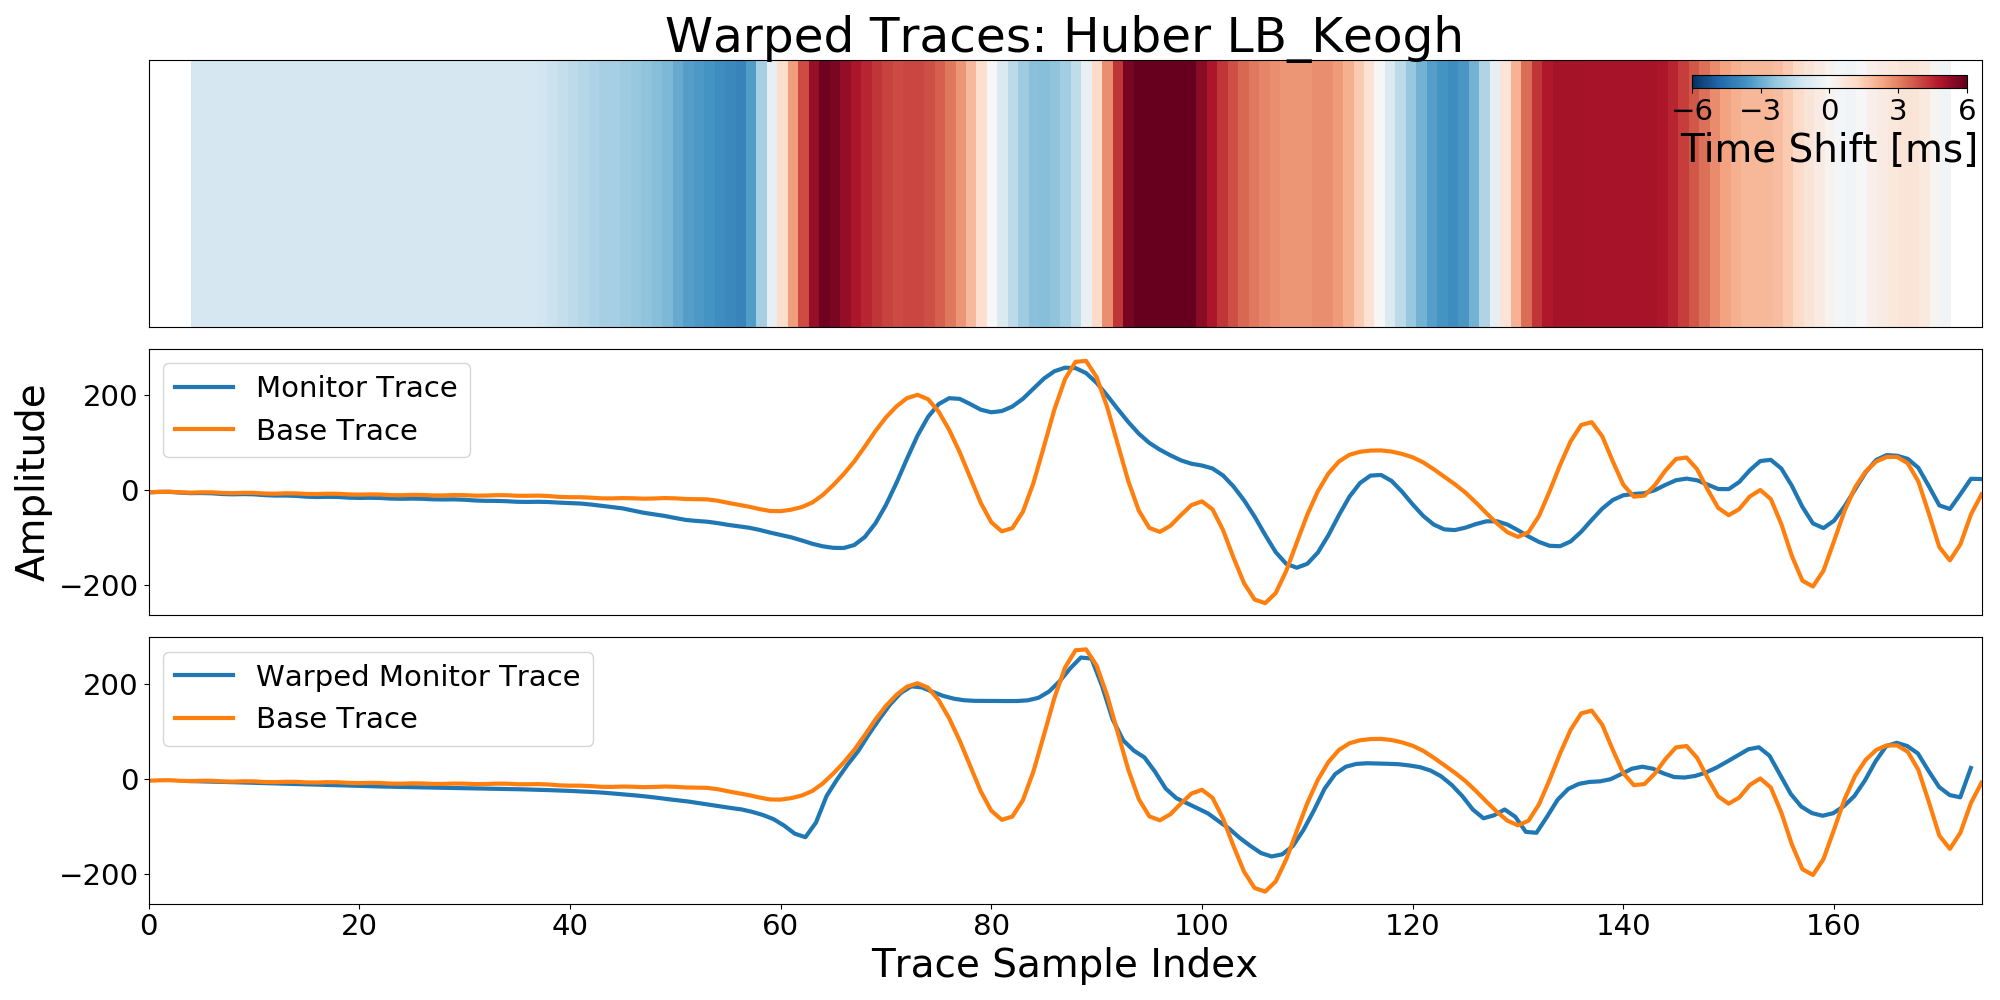
\includegraphics[width=\textwidth]{figures/time_shift_huber_lb_keogh.png}
    \caption{Time shifts and warped traces \citep[from][]{dramsch2019dtw}}
    \label{fig:time-shifts-warped}
\end{figure}

% dramsch2018information
In the workshop paper \citetitle{dramsch2018information} \citep{dramsch2018information} the insight from applying the LB\_Keogh constraint was transferable to \aclp{cnn}. \acp{cnn} apply a windowed convolution to the input data. Windowed areas of non-stationary physical data can be offset from the usually baselevel of an amplitude of zero. In the case of seismic data, traces tend to be zero-centered. In the case of a simple activation of a single neuron in a \ac{nn} with $\sigma(w\cdot x + b)$ (cf. \cref{section:nn}), this equates to a bias of $b=0$. Seismic data contains sections that fall within the range of most patches, where the reflection response is entirely offset from zero, which equates to a mean-shift within the network. This paper served as a preliminary study for \citet{dramsch2019complex}, which explores a solution for this property of patch-based training in \acp{cnn} that deteriorates the generalization.

\begin{figure}
    \centering
    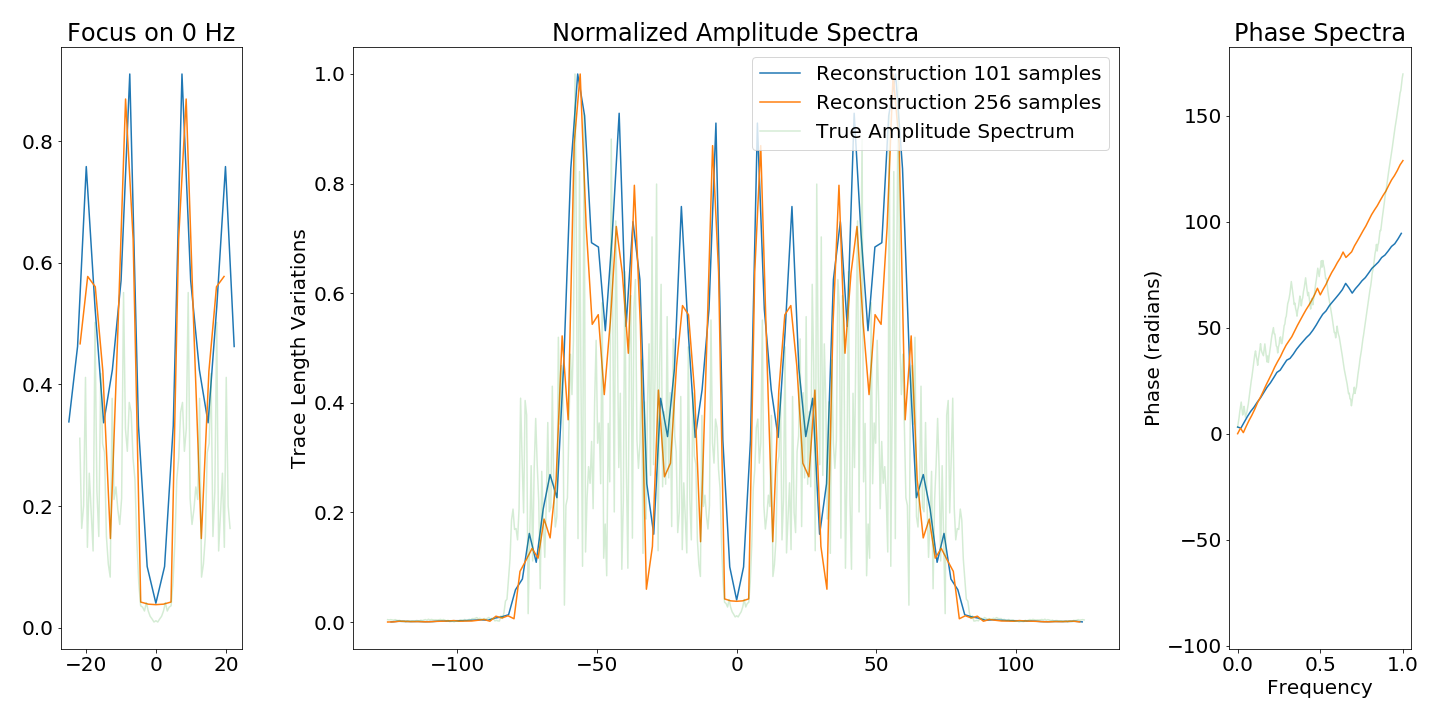
\includegraphics[width=\textwidth]{figures/information-windowing.png}
    \caption{Normalized spectra of windows of trace with "offset" zero. Aliasing of the low frequencies is visible.Phase information not reconstructed from windowed data, slope depending on the window size. Data tapered before \ac{fft} \citep[from][]{dramsch2018information}}
    \label{fig:seismic-window}
\end{figure}

\aclp{nn} apply real-valued transformations on the data, discarding phase information entirely. \cref{fig:seismic-window} shows the spectra of the full trace in green as a background, with two selected cutouts of different sizes overlaid. It is clear that both windows show a sufficiently good reconstruction of the original amplitude spectrum, except for the offset at the low frequencies. The slope of the phase spectrum is reconstructed somewhat by the larger window, but non can reconstruct the notch. Many deterministic signals contain significant information in the phase of the signal. Discarding the phase information leads to low-frequency aliasing analogous to the Nyquist-Shannon theorem for high frequencies.

% dramsch2019complex
In the paper \citetitle{dramsch2019complex} \citep{dramsch2019complex} I explore complex-valued deep convolutional networks to leverage non-linear feature maps and show that in non-stationary data, the phase content improves generalization of \acp{cnn}. Furthermore, complex-valued networks result in a smaller network with better performance compared to a larger real-valued network. In this study I implemented a deep convolutional \acl{ae} to compress 2D slices from a 3D seismic cube to evaluate the reconstruction error. There is a difference of network implementations, where complex-valued neurons are represented as two feature maps, one for the real component and complex component each. Therefore, matching the networks proved to be a complicated task, which led me to build four different architectures that get progressively bigger and compare the results.

The work in \citetitle{dramsch2019complex} \citep{dramsch2019complex} was in part based on reconstruction to test lossy compression and reconstruction of seismic data. Another reason to implement an unsupervised method was the limited availability of realiable interpretations of seismic data. Defining a decision boundary for seismic interpretation is only in the beginning stages of research, which leads us to the decision to inspect reconstructed seismic numerically as signal analysis is well-explored in seismic data processing. Therefore, analysing the result in the \ac{fk}-domain was possible and gave additional insight to the denoising effect of the \ac{ae}.

Nevertheless, some interpretations are available openly and companies often have a plethora of interpretations and re-interpretations of seismic data, making automatic seismic interpretation a topic of interest as evidenced by \cref{tab:geonn}. However, \aclp{dnn} are notorious for needing large numbers of diverse annotated samples. That is often prohibitive to geoscience applications of \acl{ml}. In \citetitle{dramsch2018deep} \citep{dramsch2018deep} we show that \aclp{sota} \aclp{cnn} pre-trained on ImageNet can be transferred to perform \acl{asi}. The pre-trained network decreases both training time and data requirements significantly, while not compromising accuracy. A pre-trained network with diverse generalizable learned filters seems to alleviate some limitations of smaller non-diverse data sets used in the fine-tuning process.

\begin{figure}[!ht]
    \subbottom[Waldeland CNN trained from scratch]{%
     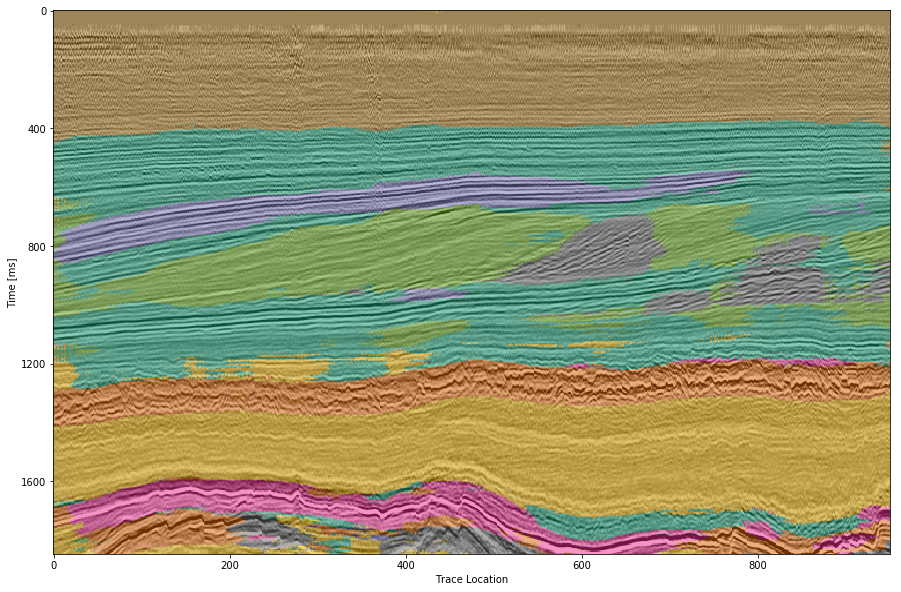
\includegraphics[width=.5\textwidth]{figures/pred1_i.png} \label{fig:asi_pred_waldeland}
    }
    \subbottom[Pre-trained VGG-16]{%
     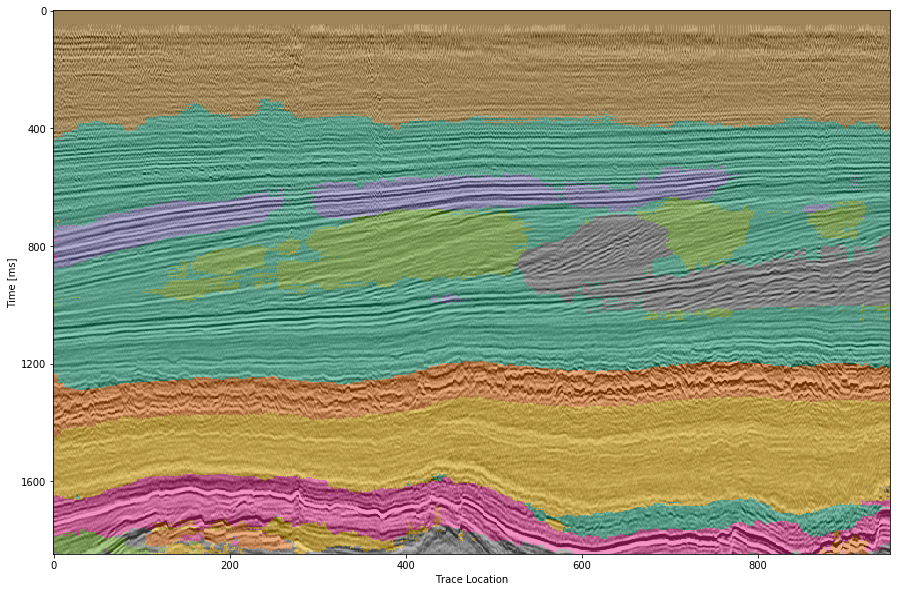
\includegraphics[width=.5\textwidth]{figures/vgg1_i.png} \label{fig:asi_pred_vgg}
    }
\caption{\acl{asi} on two networks, trained from scratch and fine-tuned on pre-trained VGG-16 architecture. The pre-trained network generating a more consistent seismic interpretation, however showing an overall deficiency in diverse training data \citep[from][]{dramsch2018deep}}
\label{fig:asi}
\end{figure}

This chapter summarizes the foundational work conducted to enable the developments of concrete applications of \acl{dl} in geophysics. These foundations touch on signal processing fundamentals in 4D seismic exploring metrics and constraints, then introducing a new constraint for \acl{dtw} in 4D seismics. The work in \aclp{dnn} includes an investigation into aliasing of patch-based training of \aclp{cnn} and including phase information in complex-valued neural networks. Finally, leading to an exploration of transfer learning for efficient training of deep learning models in \acl{asi}.

%!TEX root = ../Thesis.tex
\section{Machine Learning in 4D Seismic Inversion}

A primary application of \acl{ml} is building regression models. These regressions are suited for application in physical inversion problems, considering the value of priors in non-unique solution spaces. This chapter consists of two workshop papers that illuminate a \ac{dl} solution approach from a network architecture analysis in the paper titled \citetitle{dramsch2019including} \citep{dramsch2019including} and a data perspective in the paper titled \citetitle{dramsch2019deep} \citep{dramsch2019deep}.

\begin{figure}
    \centering
    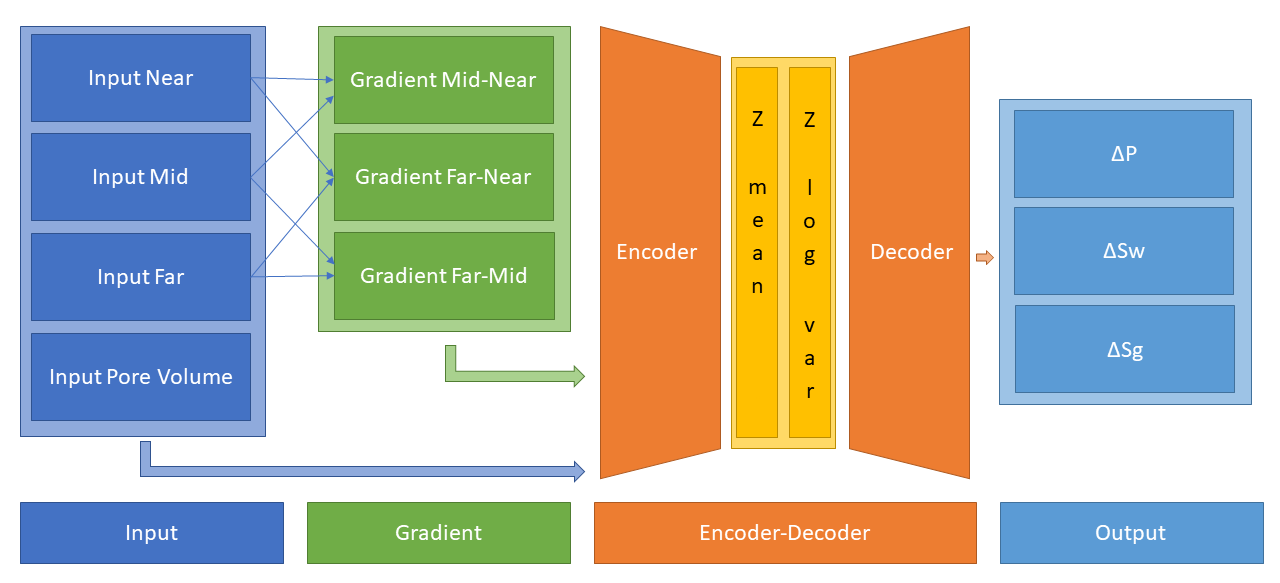
\includegraphics[width=\textwidth]{figures/AVO-Net.png}
    \caption{Architecture includes automatic physics-based gradient calculation of input seismic and an variational encoder-decoder architecture to invert seismic data for pressure and saturation changes \citep[from][]{dramsch2019including}}
    \label{fig:avo-net}
\end{figure}

Traditionally, 4D seismic \acf{qi} often relies on priors to reduce variance in the face of uncertainty. The inversion problem in this chapter is a pressure-saturation inversion from seismic amplitude difference maps in the Schiehallion field. The Schiehallion field is a stacked turbidite reservoir in the UK North Sea, which makes it very heterogeneous and compartmentalized. The T31 sandstone reservoir has the most lateral extent with the thickness ranging from 5~m to 30~m. The small thickness of the reservoir layer results in the entire reservoir being contained in a single trough of a seismic wavelet, which leads us to treat the network as a 2D map instead of a 3D problem. The data available consists of simulation and field data with several timesteps of seismic data in near-, mid-, and far-angle stacks, and pore volumes, as well as, pressure changes and saturation changes for water and gas from simulation.

In \citet{dramsch2019including} we present a novel network structure that explicitly includes AVO gradient calculation within the network as physical knowledge, shown in \cref{fig:avo-net}. The network architecture was chosen to follow an encoder-decoder architecture as a forcing function for information distillation. Additionally, the bottleneck layer implements a variational encoding layer to be less susceptible to noisy input. The network explicitly includes AVO gradient calculation in the network architecture, considering it is physical knowledge we know will stabilize pressure and saturation change separation. Including basic physics knowledge leads to the network learning residual information, essentially defining another forcing function for the networks learning process.

The initial phase was carried out on simulation data with a train test split, leaving a full 4D time step as validation set. \acl{nas} was applied to the network to determine depth and width of the architecture, using a \ac{tpe} hyper-parameter search \citep{bergstra2015hyperopt}. Afterwards, to transfer the network to field data, the input of the network was combined with additive Gaussian noise \citep{bishop1995training} to train the network for noisy field data input. This was a manual process of estimating good noise levels.
%\aclp{dnn} can learn these data-dependent priors from training data.

\begin{figure}
    \centering
    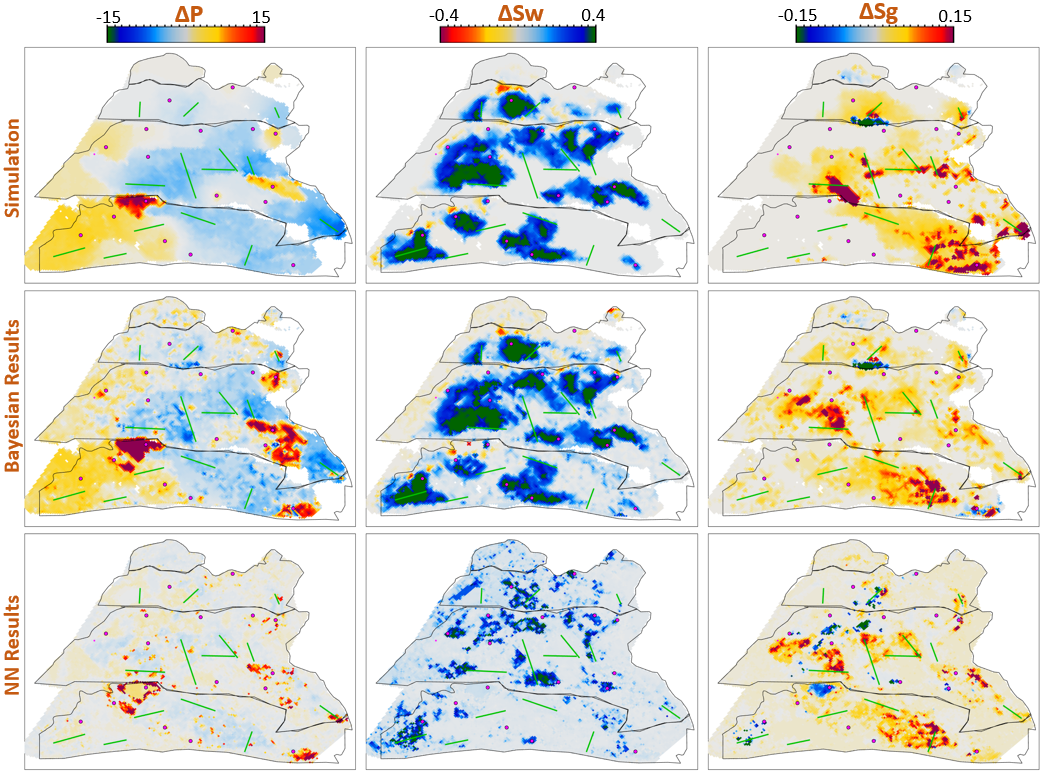
\includegraphics[width=\textwidth]{figures/NN_results.PNG}
    \caption{4D QI inversion results from Bayesian inversion and \acl{nn} inversion. Bayesian inversion closely resembles simulation output. \ac{nn} result showing good coherency, consistent amplitudes, but problems in strong changes of gas saturation \citep[from][]{dramsch2019deep}}
    \label{fig:avo-net-results}
\end{figure}

The workshop paper \citet{dramsch2019deep} contains these results compared to the simulation results and Bayesian inversion results, shown in \cref{fig:avo-net-results}. These initial results on limited training data show that the stochastic process can extract pressure saturation information from field data, after training on simulation data. While the overall result is promising, regions of strong gas saturation changes present a problem. This could be contingent problems in the modelling as well as the fact, that they generate strong amplitude differences and are far in between, essentially behaving like outliers. 

Learning meaningful information in deep neural networks is often contingent on interpreting the neural network. The results presented in \cref{fig:avo-net-results} contain three indicators that the network learned a meaningful inversion regression for the Schiehallion field. The network gets the overall trend in increase and decrease of pressure and saturation correct. Additionally, the range of output values for the network is unconstrained, but the network provides values in the ranges, that are expected from the simulation and Bayesian inversion results.  However, and more interestingly, the networks does not contain spatial information, being a feed-worward \ac{dnn} not a \ac{cnn}, yet returns continuous albeit noisy outputs when assembled into maps.

This chapter comprised of two workshop papers, shows a working implementation of a machine learning system inverting pressure-saturation data from seismic. Moreover, an implementation of a network trained on simulation data that is transferred to field data by noise modelling is presented. Finally, we show that including basic physics in the network architecture stabilizes training, making the case for physics-based \acl{ml}. Two journal papers are in preparation but not included in this thesis that analyze the network structure and the training data in detail \citep{corte2019exploring,dramsch2020physics}. 


% dramsch2019physics
% We present a novel neural network architecture that trains on synthetic data and provides insights into observed field seismic. The network explicitly includes AVO gradient calculation within the network as physical knowledge to stabilize pressure and saturation changes separation. We apply the method to Schiehallion field data and go on to compare the results to Bayesian inversion results. Despite not using convolutional neural networks for spatial information, we produce maps with good signal to noise ratio and coherency.

% dramsch2019deep
% Geoscience data often have to rely on strong priors in the face of uncertainty. Additionally, we often try to detect or model anomalous sparse data that can appear as an outlier in machine learning models. These are classic examples of imbalanced learning. Approaching these problems can benefit from including prior information from physics models or transforming data to a beneficial domain. We show an example of including physical information in the architecture of a neural network as prior information. We go on to present noise injection at training time to successfully transfer the network from synthetic data to field data.

%!TEX root = ../Thesis.tex
\section{Machine Learning in 4D Seismic Time-Shift Extraction}

This final chapter consists of the submitted journal paper \citetitle{dramsch20193dwarping}. This paper presents a novel 3D warping technique for the estimation of 4D seismic time-shifts.

4D seismic time shift extraction is often done in 1D, due to time constraints and often sub-par performance of 3D algorithms. This chapter explores and summarizes conventional 3D warping methods and machine learning approaches. Many of these algorithms rely on classical cross-correlational or optical flow approaches. These approaches suffer from the same limitations in \acl{ml} systems just like conventional algorithms. In this chapter I apply the medical Voxelmorph algorithm to match 4D seismic data.

The algorithm is trained in an unsupervised, or rather self-supervised way to avoid the bias from time shifts that were extracted from another method. The main assumption in the Voxelmorph image alignment depends on diffeomorphic warp velocity fields. The diffeomorphic assumption transfer well to the geological reality that the the mathematical topology stays constant, resulting in reflectors neither crossing nor generating loops. 

\begin{figure}
    \centering
    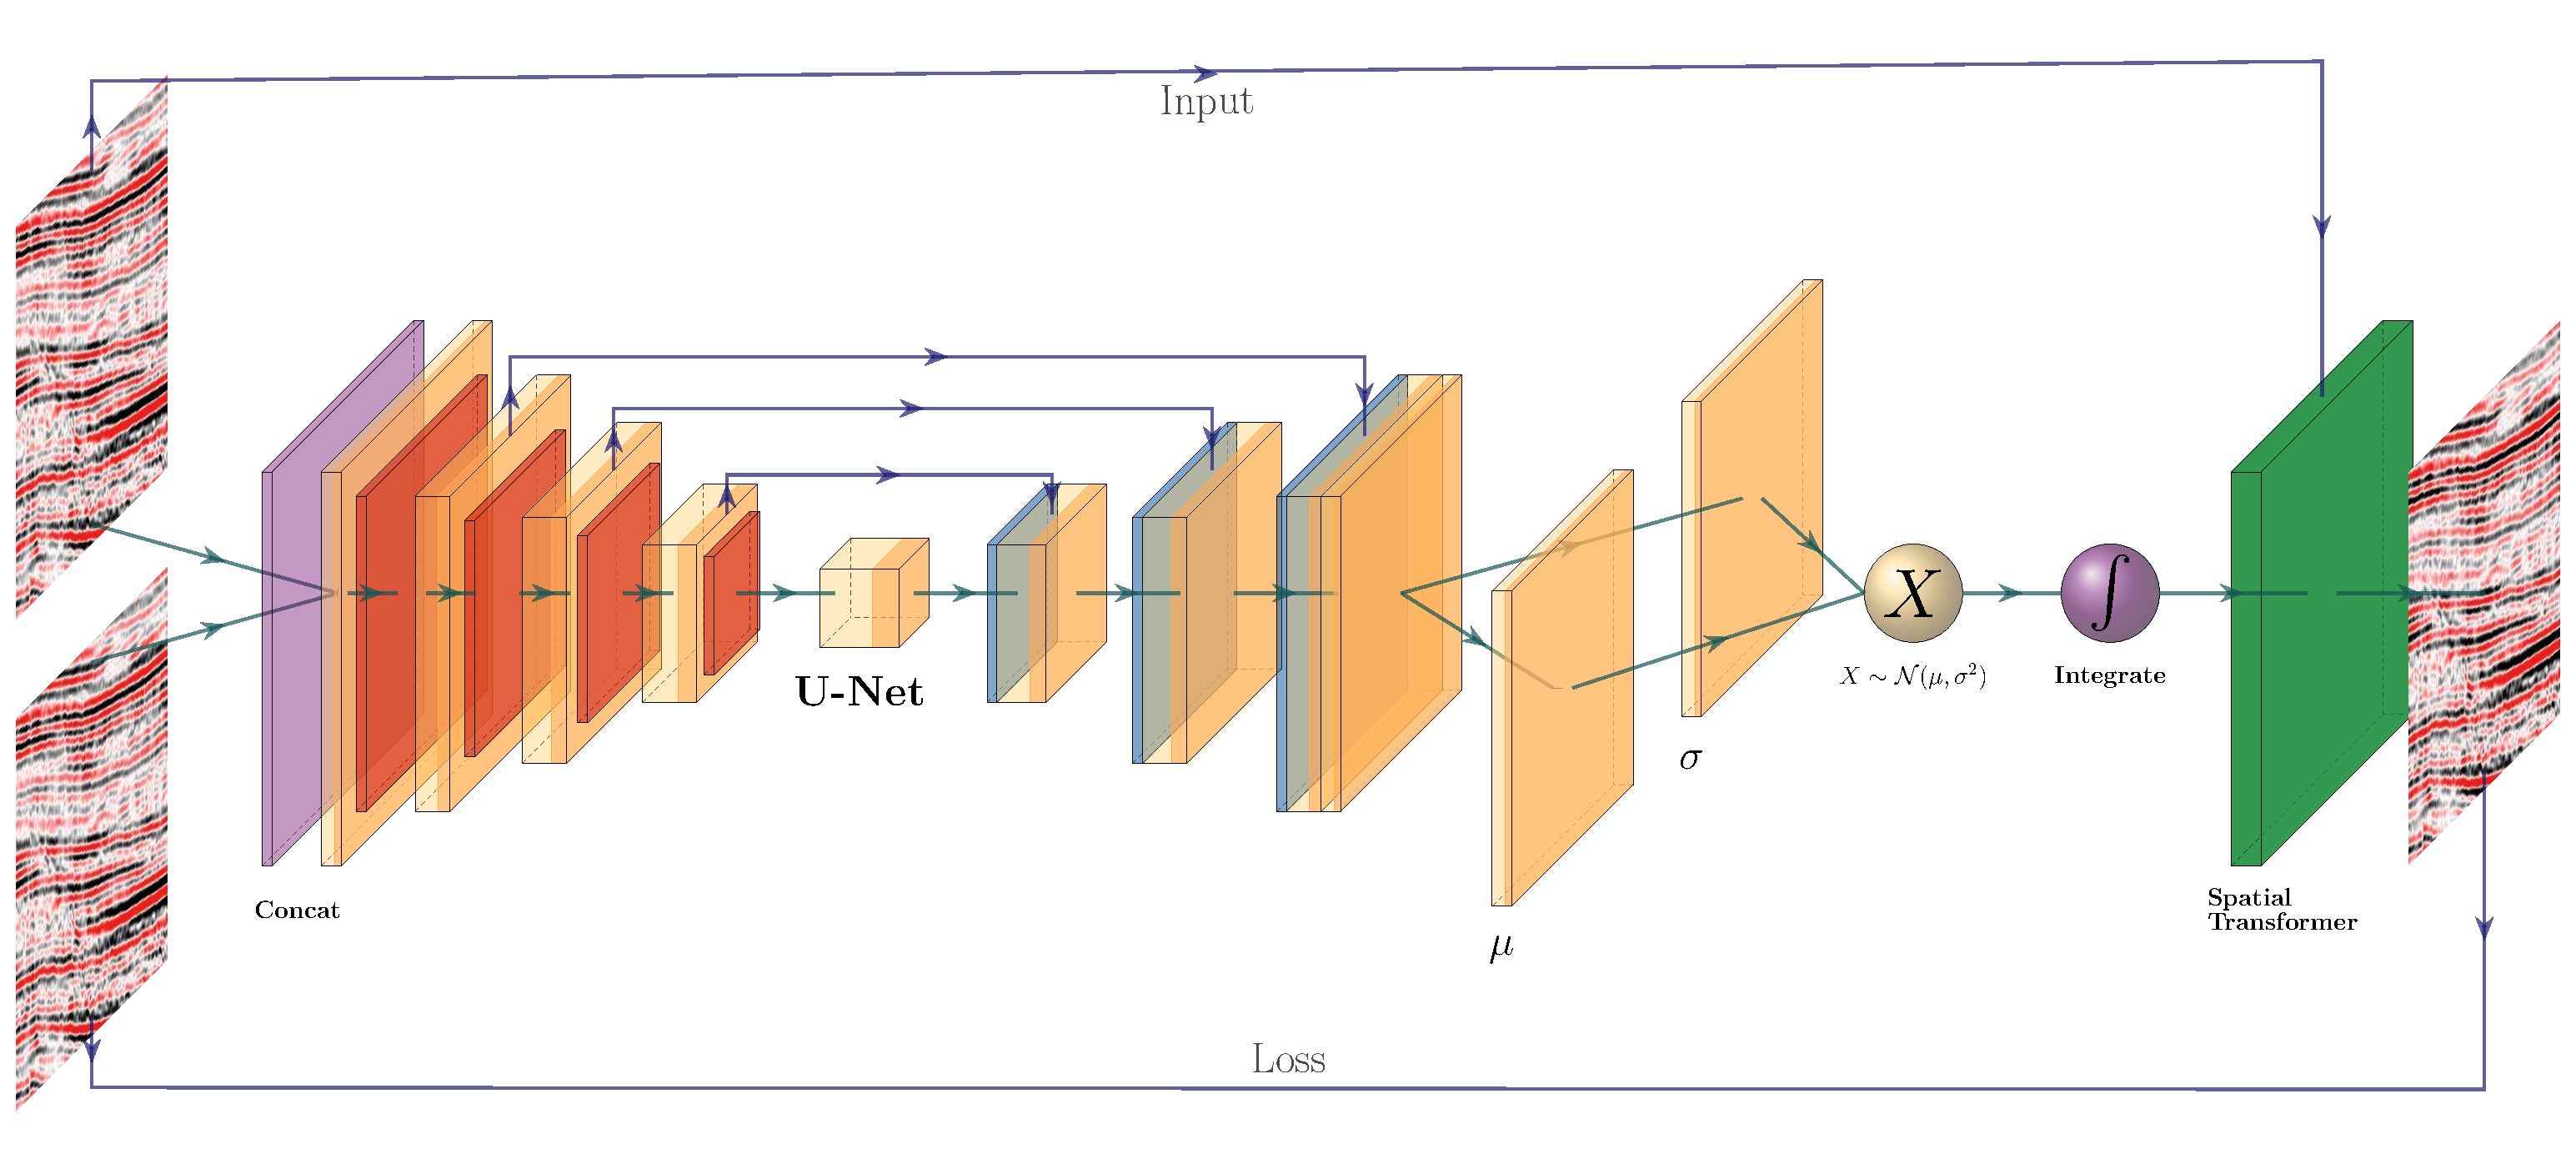
\includegraphics[width=\textwidth]{figures/Voxelmorph.pdf}
    \caption{Voxelmorph Architecture}
    \label{fig:voxelmorph}
\end{figure}
\todo{Extend Description}

The architecture in the network uses the U-Net architecture to input two 3D seismic volumes and extract a static warp velocity field, shown in \cref{fig:voxelmorph}. The static velocity field is extracted as a Gaussian distribution to measure the co-variance and provide uncertainty value of the three-dimensional warp field. The neural network itself does not warp the seismic data, to increase transparency of the process. The architecture following the U-net samples the extracted velocity distribution and integrates this value to obtain the diffeomorphic flow. These values are passed to a dense 3D warping mechanism to enable the unsupervised training. The losses involved are a \acf{kl} on the stationary velocity field and \ac{mse} on the difference between that warped monitor volume and the base volume.

In the paper we present the modified self-supervised \acl{nn} system and test the results on the training data itself and two generalization test sets. The first test set is on the same field but recorded at different times to the training set, ensuring a similar underlying geology, whereas, the second test set is taken from an adjacent field, recorded at different times, testing the full transfer of the trained network. We go on to test the original Voxelmorph architecture, which uses upsampled velocity fields and evaluate the results against our modified architecture, which uses the full flow field. Overall, this technique introduces a generalizable \acl{dl} approach to extract 3D time-shifts with uncertainty measures from raw stacked 4D seismic data.

\section{Contributions of this Study}



\chapter{Data Preparation and Analysis}
\label{sec:dataprep}
% %!TEX root = ../Thesis.tex
%\chapter{Long chapter title with $\pi$ $π$ or π}
%\chapter{Long chapter title with \texorpdfstring{$\pi$ $π$ or π}{π π or π}}
\section{Correlation of Fractures From Core, Borehole Images and Seismic Data in a Chalk Reservoir in the Danish North Sea}
\label{seg:talaEAGE}
\paragraph{Abstract:} We present an integrated fracture study in the Ekofisk chalk reservoir of the Kraka Field, offshore Denmark, based on core, borehole images and seismic data. The core contains numerous fractures ranging from short (cm-scale) fractures, mostly associated with chert or stylolites, to large (m-scale) open, slickensided fractures likely related to halokinesis. On borehole images, especially larger fractures are identified, coinciding in dip and dip-azimuth. Seismic data at an approximate resolution of 40m would not resolve these local features around the well-bore. We show that chromatic analysis combined with an ant-tracking algorithm extracts several lineaments (> m-scale) from the seismic data. These correlate closely in orientation and distribution with the fractures logged in the well data. It is likely that these represent fracture corridors, small faults or damage zones in the chalk. The seismic data therefore provides a valuable method for mapping the size, orientation and connectivity of fracture zones away from the well. This gives insights into the scalability of local stress fields, and fracture distributions. 

{\vfill\hfill\newline\fbox{\parbox{.97\textwidth}{\fullcite{aabo2017correlation}}}}

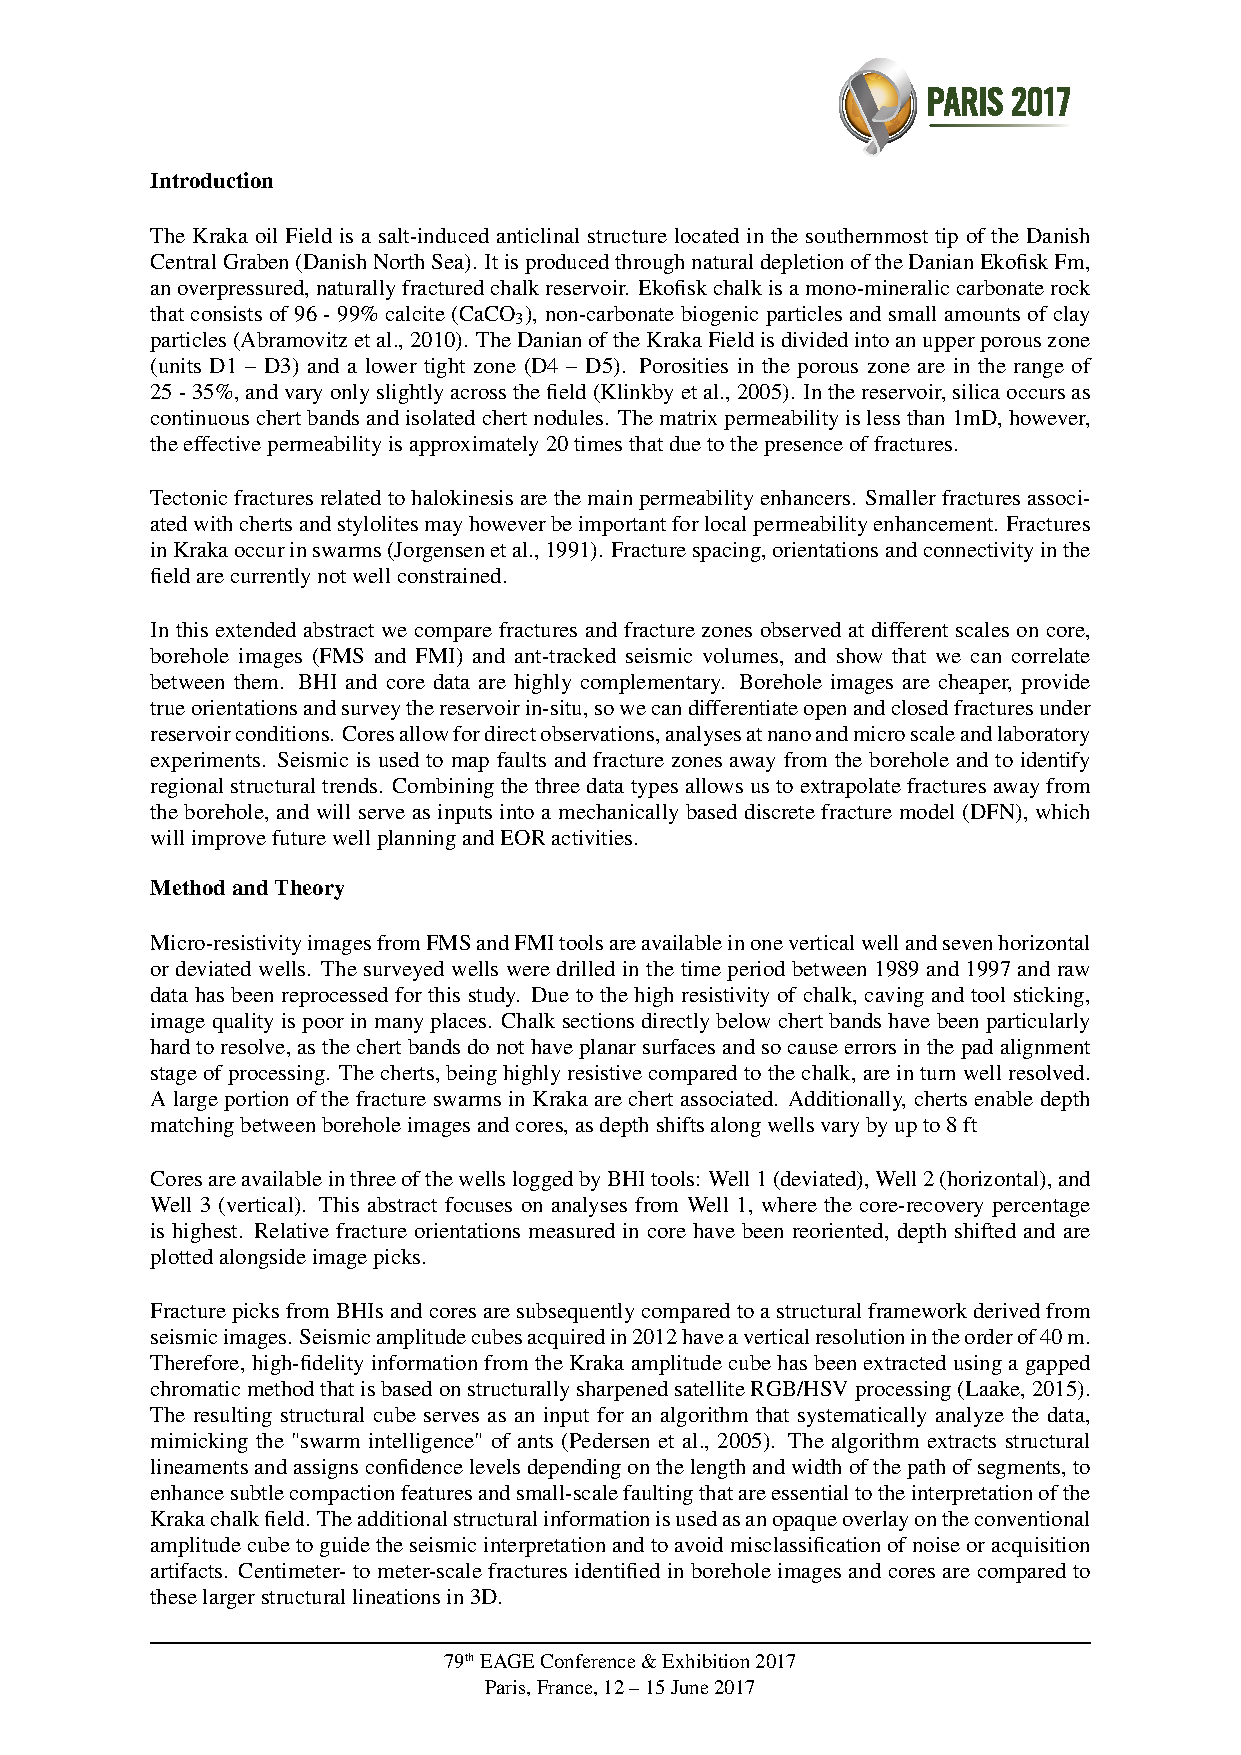
\includepdf[pages=1-4,pagecommand={},width=1.2\textwidth,offset=0.7cm -1.5cm]{papers/2017.1}

\todo{Fix Alignment}
% %!TEX root = ../Thesis.tex
%\chapter{Long chapter title with $\pi$ $π$ or π}
%\chapter{Long chapter title with \texorpdfstring{$\pi$ $π$ or π}{π π or π}}
\section{An Integrated Approach to Fracture Characterization of the Kraka Field}
\label{seg:tala}

\paragraph{Abstract:} Oil and gas production of tight chalk reservoirs frequently rely on the presence of natural fractures, which increases the effective permeability of the reservoirs.  Knowledge of these fracture systems can therefore be used strategically in well planning as well as in IOR and EOR efforts.  Here we present an integrated workflow for fracture characterization in chalk, developed in the Kraka Field, located in the Danish sector of the North Sea.  The workflow is based on data from borehole images, cores and seismic.  By introducing two ant-tracked attribute volumes, which display structural trends below the resolution of amplitude seismic, we are able to correlate features at different scales.  In Kraka, this approach has revealed that the fracture pattern is more complex than previously suggested.  We propose that fracture generation and propagation in the field is in part controlled by the regional maximum horizontal stress and in part formed in response to salt movements.

{\vfill\hfill\newline\fbox{\parbox{.97\textwidth}{\fullcite{aabo2018integrated}}}}

\includepdf[pages=1-12,pagecommand={},width=1.2\textwidth,offset=0.7cm 0.1cm]{papers/2018.1}
\todo{Fix Alignment} 
% %!TEX root = ../Thesis.tex
%\chapter{Long chapter title with $\pi$ $π$ or π}
%\chapter{Long chapter title with \texorpdfstring{$\pi$ $π$ or π}{π π or π}}
\section[Gaussian Mixture Models for Robust Unsupervised Scanning-Electron Microscopy Image Segmentation of North Sea Chalk]{Gaussian Mixture Models for Robust Unsupervised Scanning-Electron Microscopy Image Segmentation of North Sea Chalk}
\label{section:gaussian}
\paragraph{Abstract:} Scanning-Electron images from North Sea Chalk are studied for important rock properties. To relieve this manual labor, we investigated several standard image processing methods that underperformed on complicated chalk. Due to the lack of manually labeled data, deep neural networks could not be adequately applied. Gaussian Mixture Models learnt a two-fold representation that separated the background well from the rock. Subsequent morphological filtering cleans up the prediction and enables automatic analysis. 

{\vfill\hfill\newline\fbox{\parbox{.97\textwidth}{\fullcite{dramsch2018gaussian}}}}
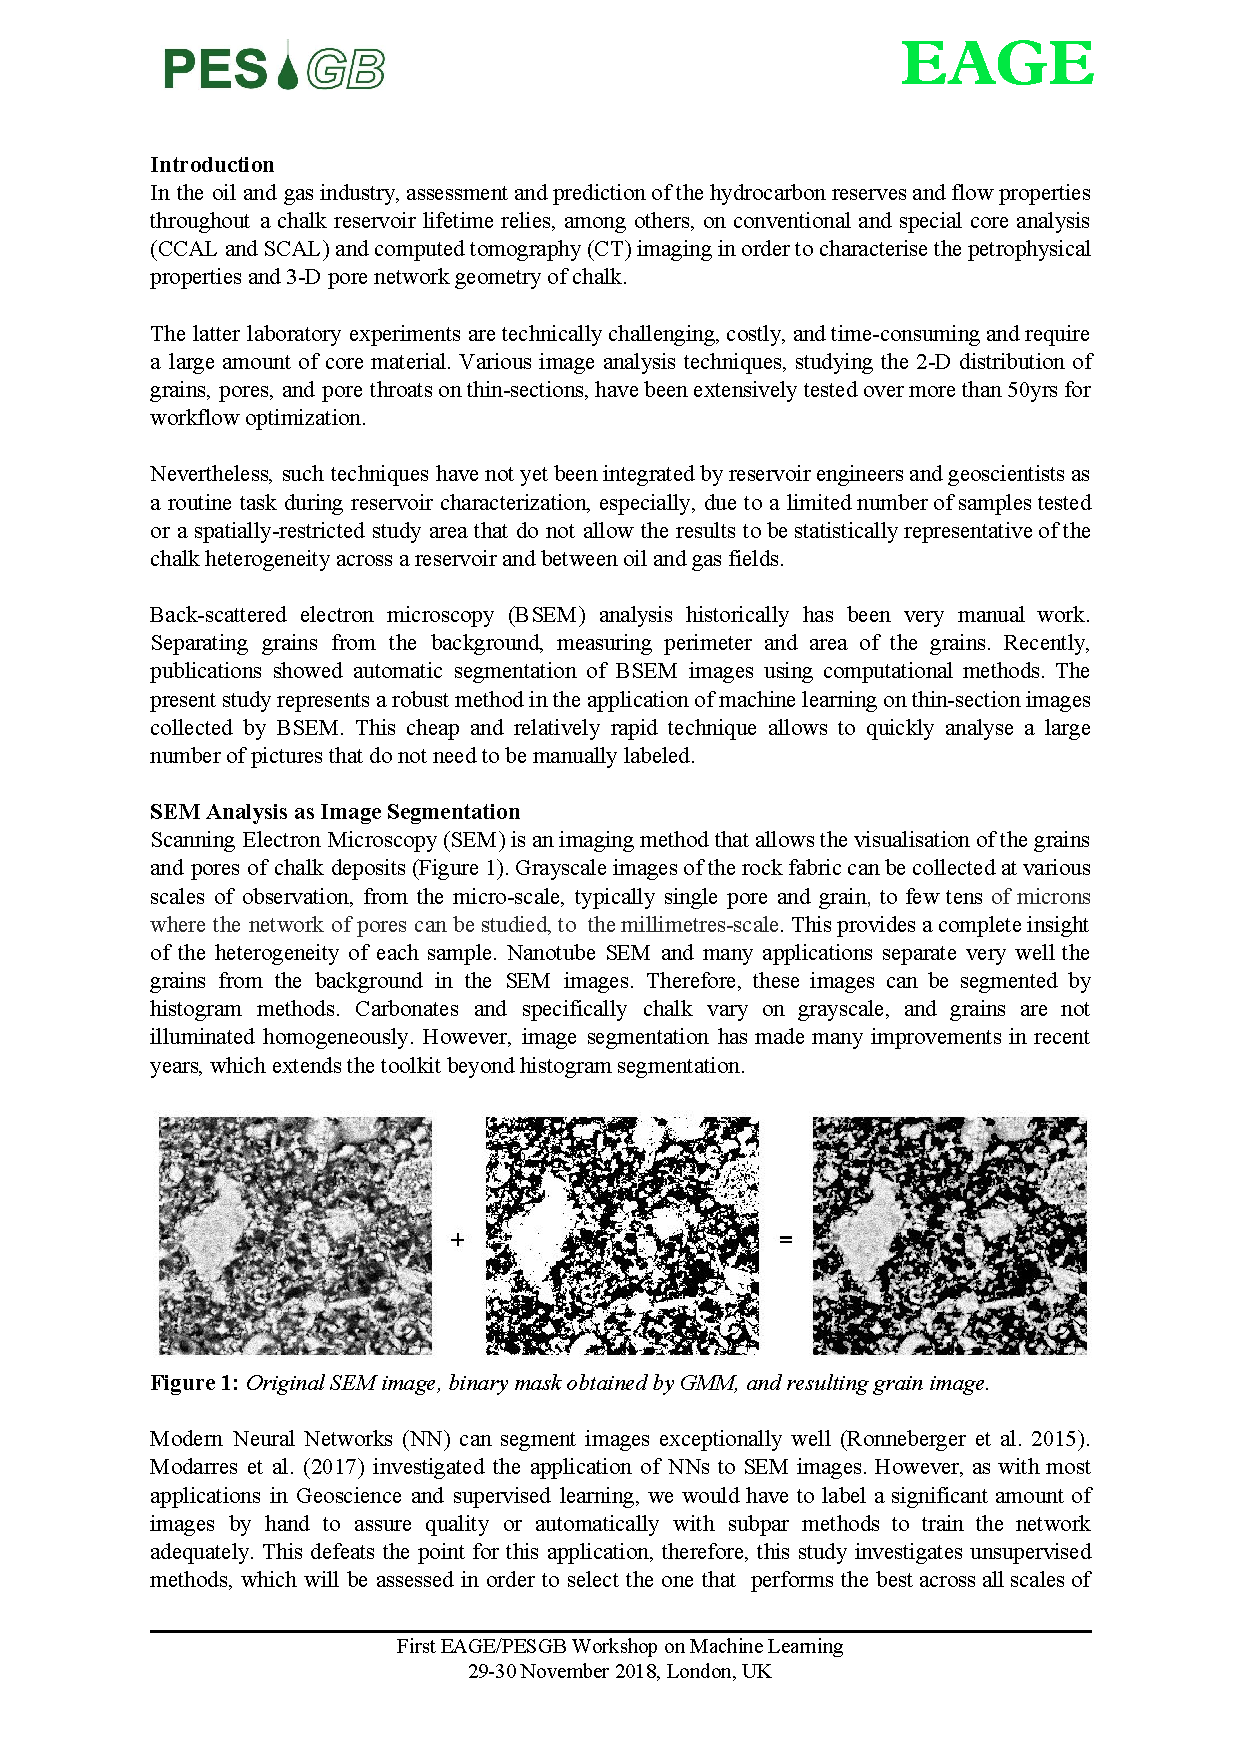
\includepdf[pages=1-2,pagecommand={},width=1.2\textwidth,offset=0.7cm -1.5cm]{papers/2018.2}

\chapter{Foundations of Deep Learning for Seismic Data Analysis}
\label{sec:foundations}
% %\section[Dynamic Time Warping Tutorial Paper]{Let's do the Time Warp again!}
\section[Dynamic Time Warping Tutorial Paper]{Revisiting Dynamic Time Warping -- A practical tutorial in Python on North Sea field data}

\paragraph{Abstract:} This tutorial revisits Dynamic Time Warping for geoscientific applications.  This algorithm can be used to match arbitrary time-series, which is applicable to 4D time shifts, seismic-well ties, well-to-well ties, and seismic pre- and post-stack migration.  DTW is notorious to be computationally slow and expensive, while under-performing on seismic field data.  We show that a choice of similarity measures, optimization, and constraints can both speed up calculation and significantly improve results.  We show a full implementation in Python code on 4D seismic traces recorded over 10 years apart. Moreover, we explore recent developments in DTW and the significance to machine learning metrics

{\vfill\hfill\newline\fbox{\parbox{.97\textwidth}{\fullcite{dramsch2019dtw}}}}

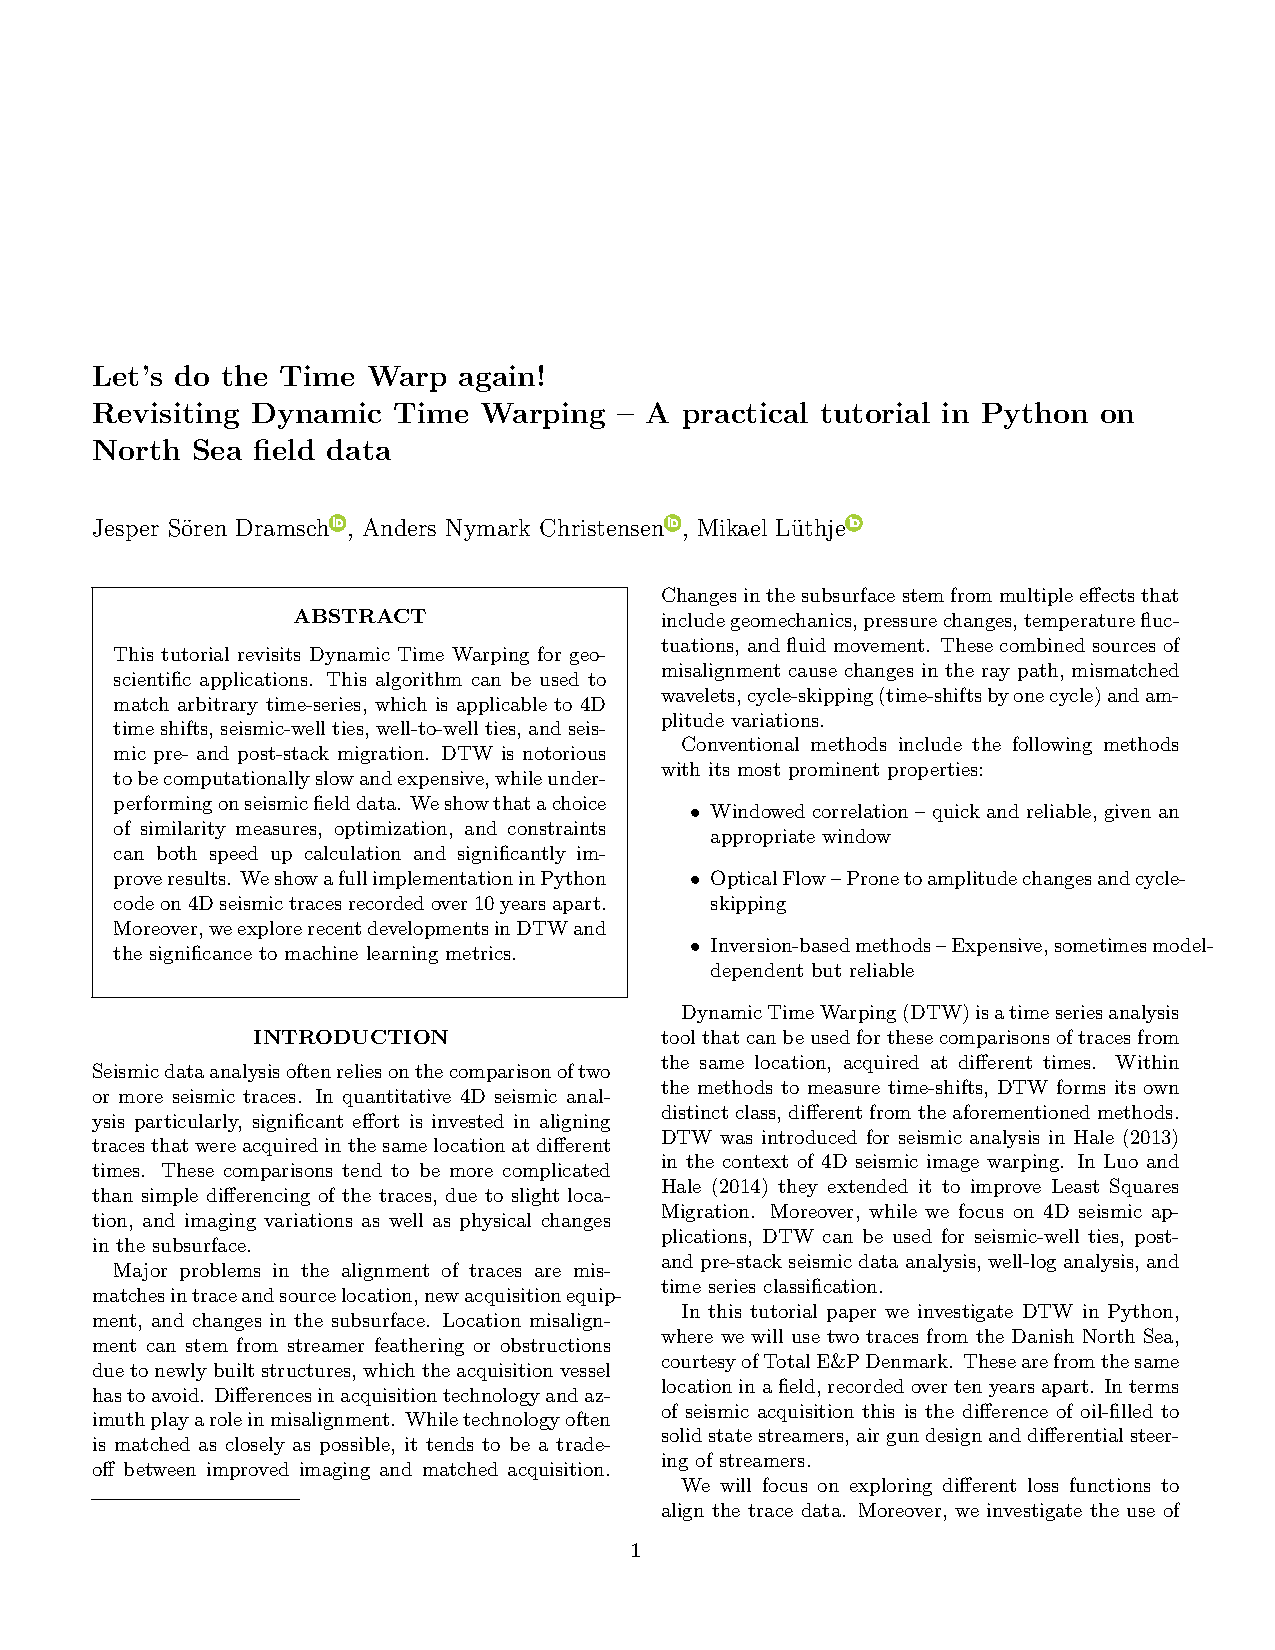
\includepdf[pages=1-11,pagecommand={},width=1.2\textwidth,offset=0.7cm 0.1cm]{papers/2019.4}
\todo{Check Page Numbers}
\todo{Fix Alignment}

% %!TEX root = ../Thesis.tex
%\chapter{Long chapter title with $\pi$ $π$ or π}
%\chapter{Long chapter title with \texorpdfstring{$\pi$ $π$ or π}{π π or π}}
\chapter[Complex-valued neural networks for machine learning on non-stationary physical data]{Complex-valued\\neural networks\\for machine learning on\\\hspace*{-2cm}non-stationary physical data}

\todo{Include Abstract}

{\vfill\hfill\newline\fbox{\parbox{.97\textwidth}{\fullcite{dramsch2019complex}}}}
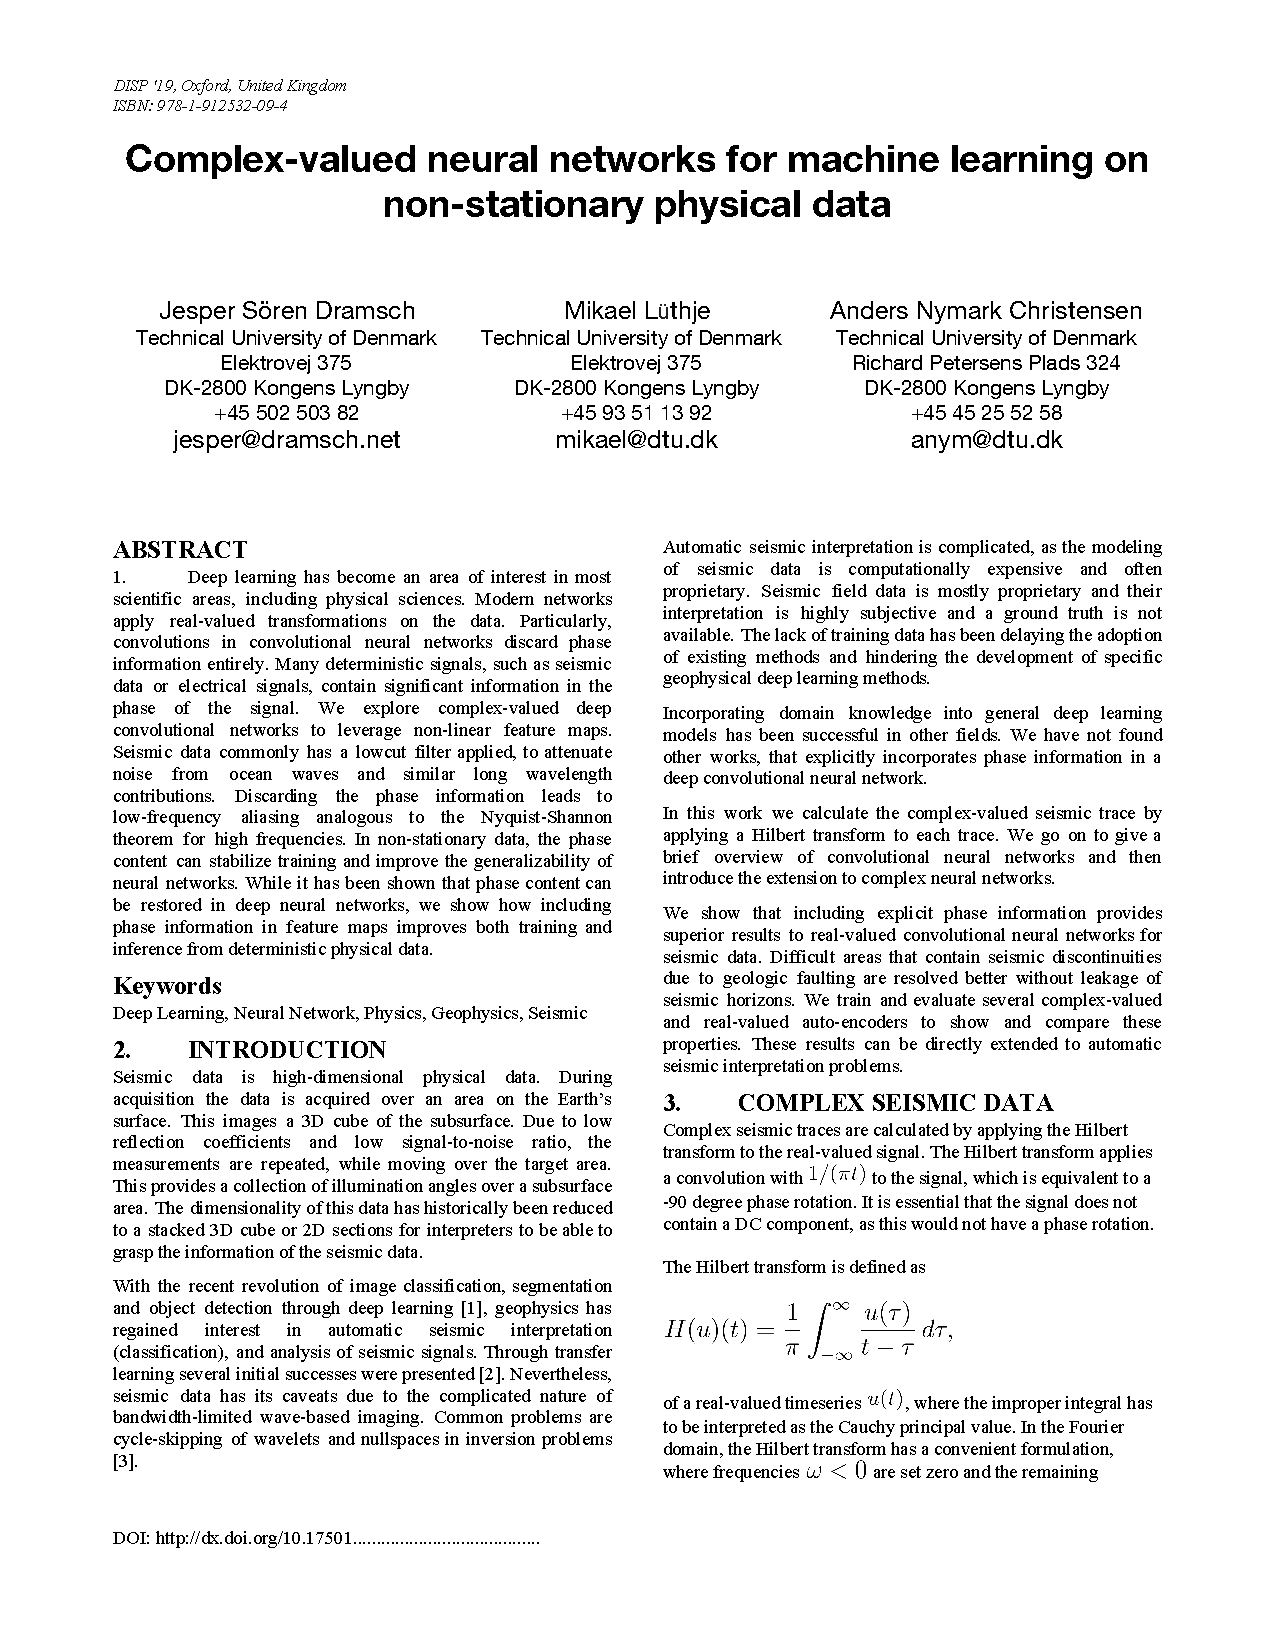
\includepdf[pages=1-6,pagecommand={},width=1.2\textwidth,offset=0.7cm 0.1cm]{papers/2019.1}
\todo{Check Page Numbers}
\todo{Fix Alignment}
% %!TEX root = ../Thesis.tex
%\chapter{Long chapter title with $\pi$ $π$ or π}
%\chapter{Long chapter title with \texorpdfstring{$\pi$ $π$ or π}{π π or π}}
\section{Information Theory Considerations in Patch-based Training of Deep Neural Networks on Seismic Time-Series}

\paragraph{Abstract:} Recent advances in machine learning relies on convolutional deep neural networks. These are often trained on cropped image patches. Pertaining to non-stationary seismic signals this may introduce low frequency noise and non-generalizability.

{\vfill\hfill\newline\fbox{\parbox{.97\textwidth}{\fullcite{dramsch2018information}}}}

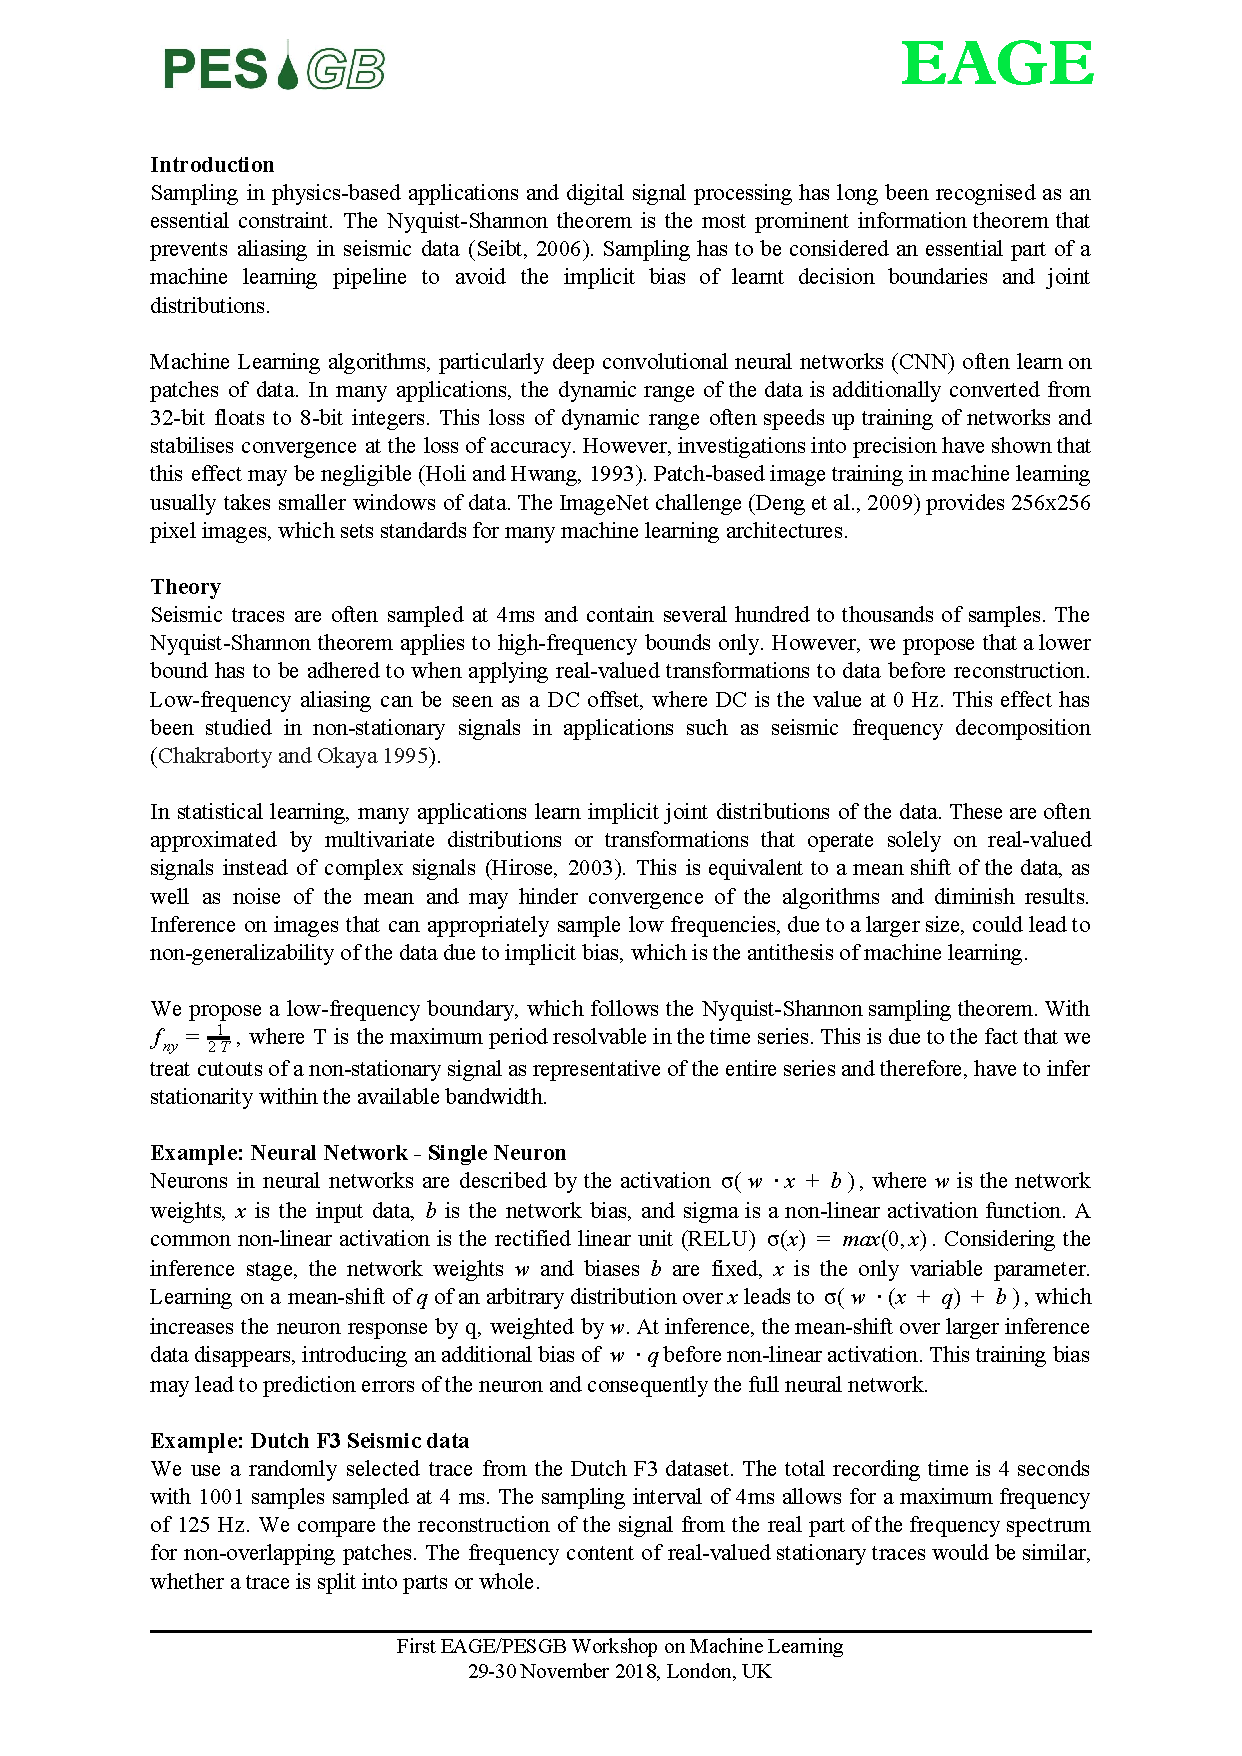
\includepdf[pages=1-2,pagecommand={},width=1.2\textwidth,offset=0.7cm -1.5cm]{papers/2018.3}
\todo{Check Page Numbers}
\todo{Fix Alignment}
% %!TEX root = ../Thesis.tex
%\chapter{Long chapter title with $\pi$ $π$ or π}
%\chapter{Long chapter title with \texorpdfstring{$\pi$ $π$ or π}{π π or π}}
\chapter{Deep learning seismic facies on state of the art CNN architectures}

We explore propagation of seismic interpretation by deep learning in stacked 2D sections. We show the application of state-of-the-art image classification algorithms on seismic data. These algorithms were trained on big labeled photograph databases. We use transfer learning to benefit from pre-trained networks and evaluate their performance on seismic data.

{\vfill\hfill\newline\fbox{\parbox{.97\textwidth}{\fullcite{dramsch2018deep}}}}

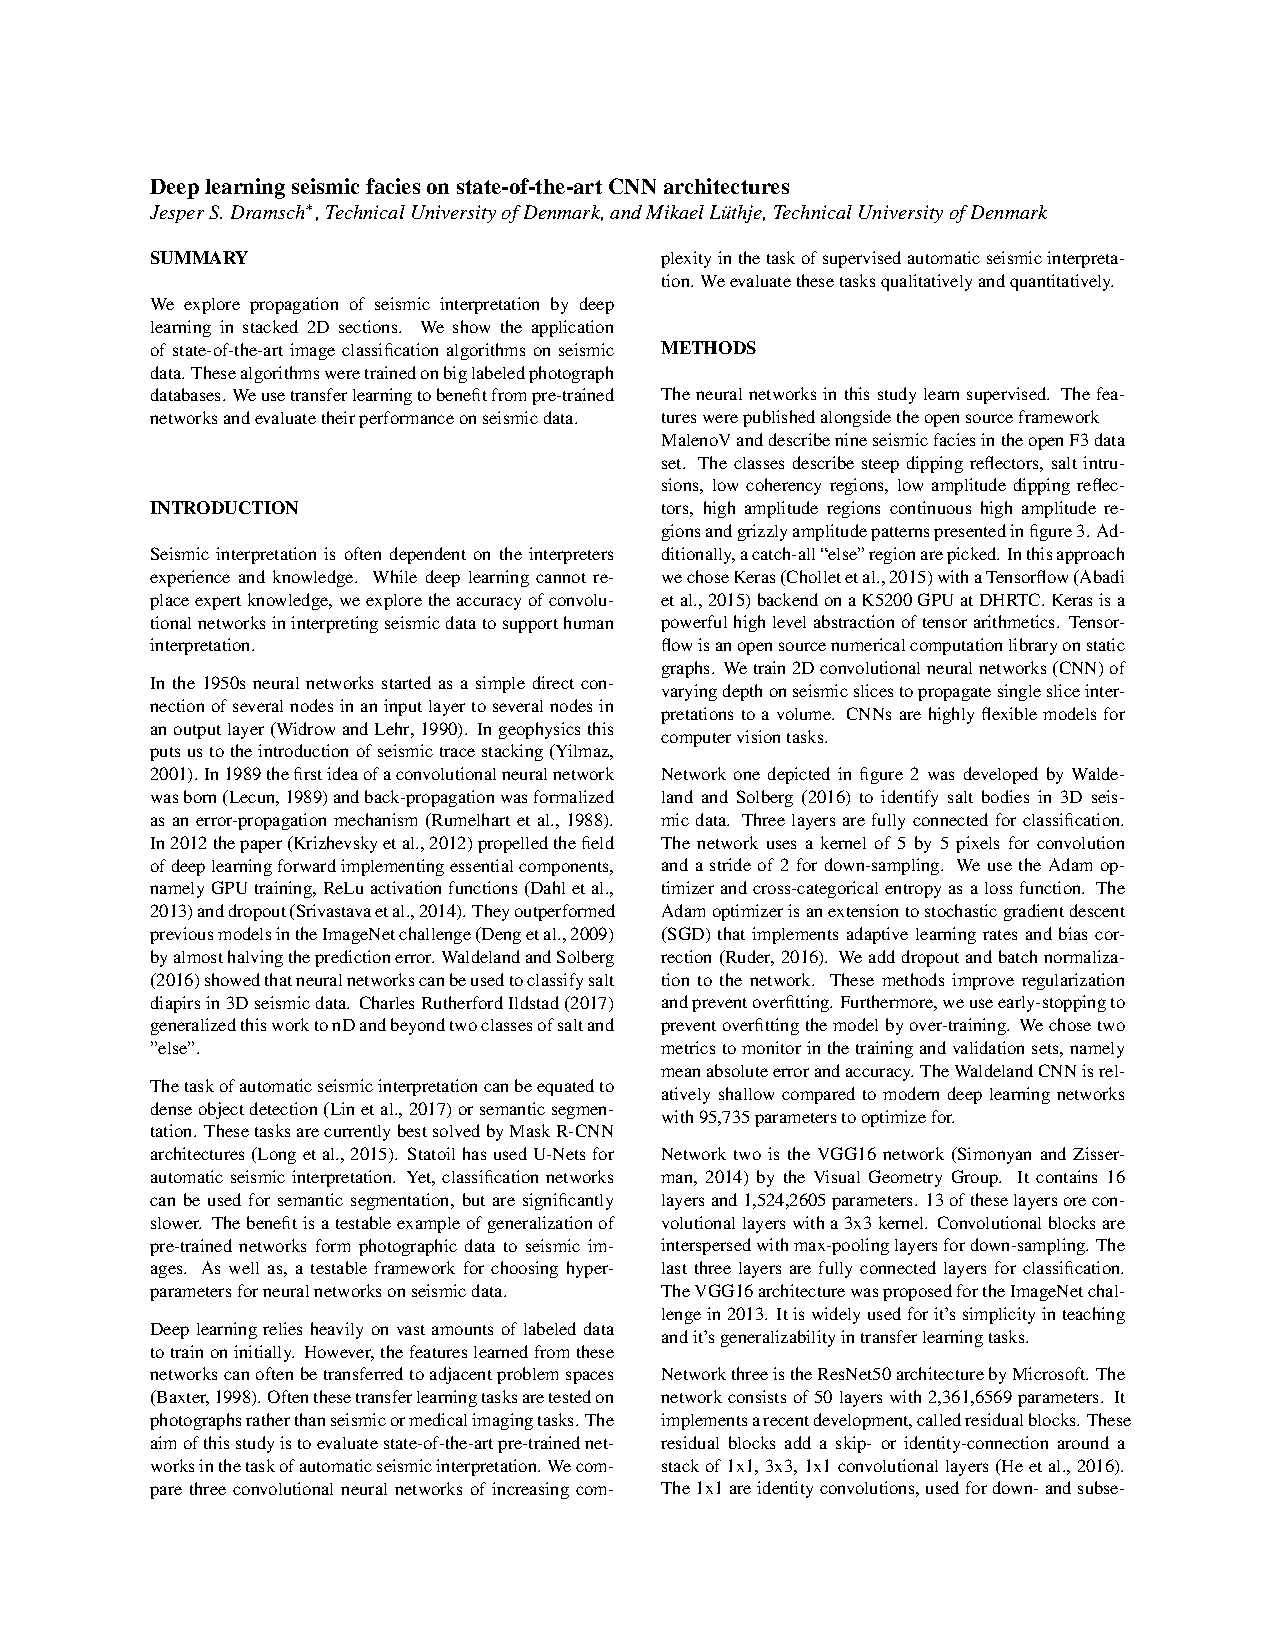
\includepdf[pages=1-4,pagecommand={},width=1.2\textwidth,offset=0.7cm -1.5cm]{papers/2018.4}
\todo{Check Page Numbers}
\todo{Fix Alignment}


\chapter{Deep Neural Networks for 4D Seismic Inversion}
\label{sec:inversion}
% %!TEX root = ../Thesis.tex
%\chapter{Long chapter title with $\pi$ $π$ or π}
%\chapter{Long chapter title with \texorpdfstring{$\pi$ $π$ or π}{π π or π}}
\chapter[Including Physics in Deep Learning – An Example from 4D Seismic Pressure Saturation Inversion]{Including Physics in\\Deep Learning\\An Example from\\4D Seismic Pressure Saturation Inversion}

\todo{Include Abstract}
{\vfill\hfill\newline\fbox{\parbox{.97\textwidth}{\fullcite{dramsch2019physics}}}}
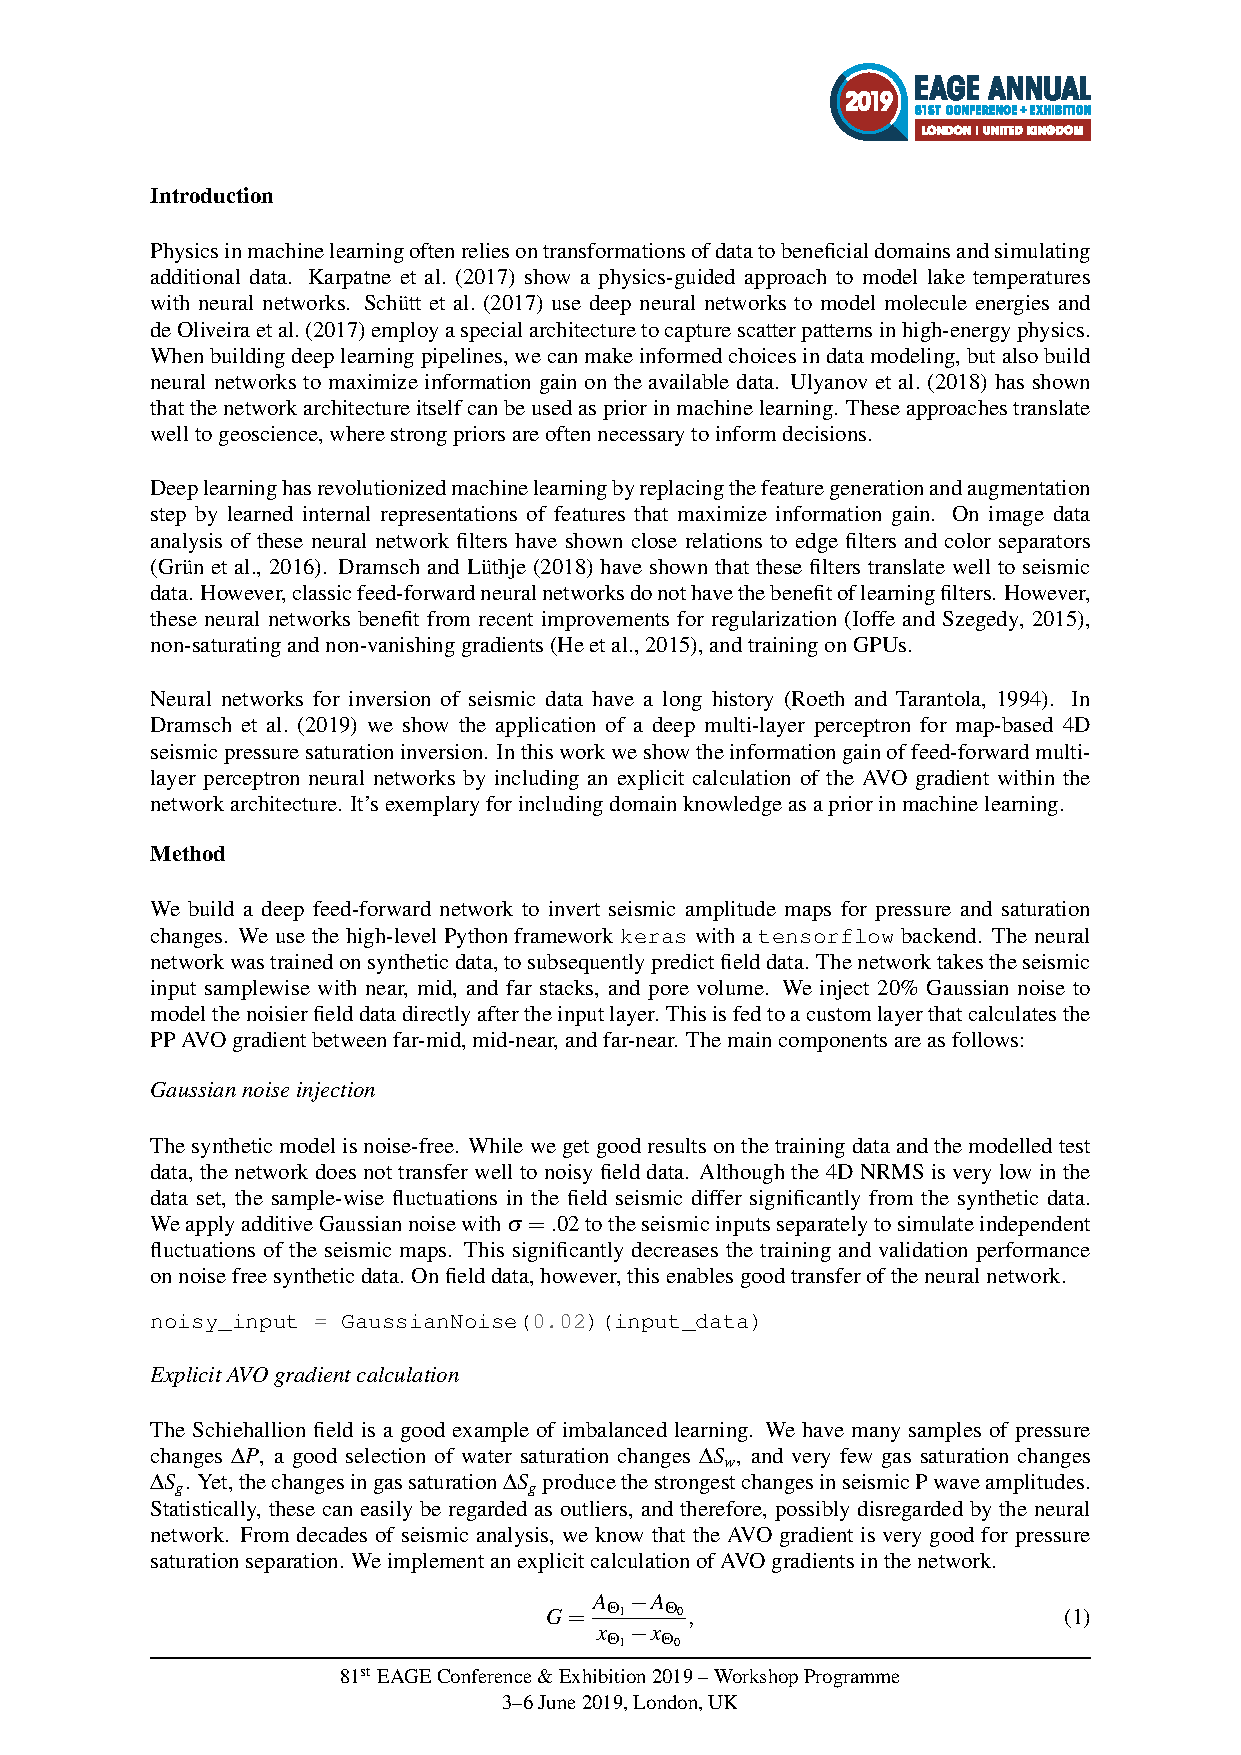
\includepdf[pages=1-4,pagecommand={},width=1.2\textwidth,offset=0.7cm -1.5cm]{papers/2019.3}


\todo{Check Page Numbers}
\todo{Fix Alignment}
% %!TEX root = ../Thesis.tex
%\chapter{Long chapter title with $\pi$ $π$ or π}
%\chapter{Long chapter title with \texorpdfstring{$\pi$ $π$ or π}{π π or π}}
\section[Deep Learning Application for 4D Pressure Saturation Inversion Compared to Bayesian Inversion on North Sea Data]{Deep Learning Application\\for 4D Pressure Saturation Inversion Compared to Bayesian Inversion on\\North Sea Data}

\paragraph{Abstract:} In this work we present a deep neural network inversion on map-based 4D seismic data for pressure and saturation. We present a novel neural network architecture that trains on synthetic data and provides insights into observed field seismic. The network explicitly includes AVO gradient calculation within the network as physical knowledge to stabilize pressure and saturation changes separation. We apply the method to Schiehallion field data and go on to compare the results to Bayesian inversion results. Despite not using convolutional neural networks for spatial information, we produce maps with good signal to noise ratio and coherency.

{\vfill\hfill\newline\fbox{\parbox{.97\textwidth}{\fullcite{dramsch2019deep}}}}

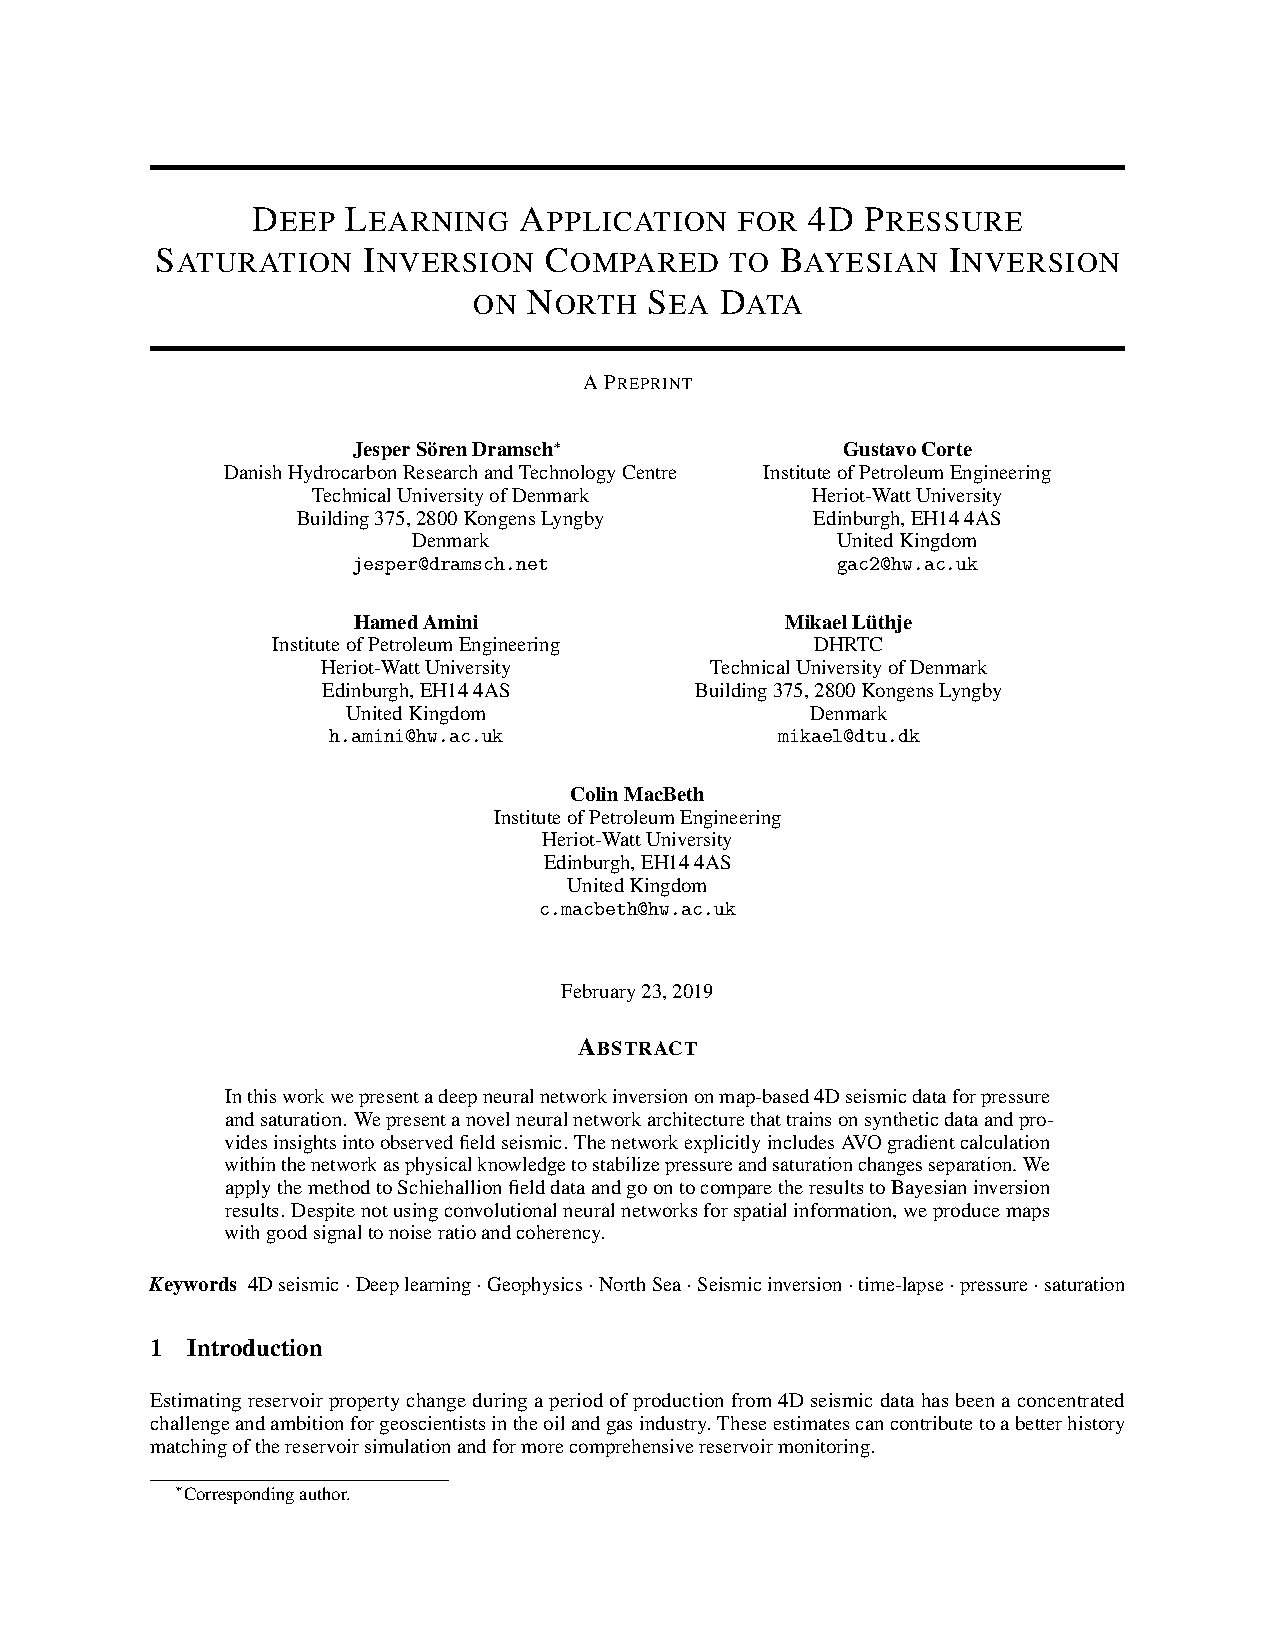
\includepdf[pages=1-5,pagecommand={},width=1.2\textwidth,offset=0.7cm -1.5cm]{papers/2019.2}
\todo{Check Page Numbers}
\todo{Fix Alignment}

\chapter{Deep Convolutional Networks for 4D Time Shift Extraction}
\label{sec:timeshift}
%  include{chapters/Paper3DWarping}

%%!TEX root = ../Thesis.tex
\chapter{Conclusion}
Morbi pharetra ligula integer mollis mi nec neque ultrices vitae volutpat leo ullamcorper. In at tellus magna. Curabitur quis posuere purus. Cum sociis natoque penatibus et magnis dis parturient montes, nascetur ridiculus mus. Suspendisse tristique placerat feugiat. Aliquam vitae est at enim auctor ultrices eleifend a urna. Donec non tincidunt felis. Maecenas at suscipit orci.


\appendix

%!TEX root = ../Thesis.tex
\chapter{ImageNet Results}
\vspace*{-12pt}
\begin{longtabu} to \textwidth {ll|r|r|r}
\toprule
Name & Citation & Top-1 [\%] & Top-5 [\%] & Param [M] \\
\bottomrule
\toprule
AlexNet         & \citet{krizhevsky2012imagenet} & 63,3    & 84,6   &  60  \\
\bottomrule
VGG-16          & \citet{simonyan2014very}       & 74,4    & 91,9    & 138     \\
VGG-19          & \citet{simonyan2014very}       & 74,5    & 92,0    & 144    \\
\bottomrule
AmoebaNet-B   & \citet{real2019regularized}    & 82,3    & 96,1    & 84      \\
AmoebaNet-C   & \citet{real2019regularized}    & 83,1    & 96,3    & 155,3      \\
\bottomrule
DenseNet-201  & \citet{huang2017densely}       & 78,5    & 94,4    & 20      \\
\bottomrule
EfficientNet-B1  & \citet{tan2019efficientnet}  & 78,8     & 94,4     & 7,8     \\
EfficientNet-B2  & \citet{tan2019efficientnet}  & 79,8     & 94,9     & 9,2      \\
EfficientNet-B3  & \citet{tan2019efficientnet}  & 81,1     & 95,5     & 12      \\
EfficientNet-B4  & \citet{tan2019efficientnet}  & 82,6     & 96,3     & 19      \\
EfficientNet-B5  & \citet{tan2019efficientnet}  & 83,3     & 96,7     & 30      \\
EfficientNet-B6  & \citet{tan2019efficientnet}  & 84,0     & 96,9     & 43      \\
EfficientNet-B7  & \citet{tan2019efficientnet}  & 85,0     & 97,2     & 66      \\
\bottomrule
Inception V1        & \citet{szegedy2015going}       & 69,8     & 89,9     & 5      \\
Inception V2        & \citet{ioffe2015batch}         & 74,8     & 92,2     & 11,2      \\
Inception V3        & \citet{szegedy2016rethinking}  & 78,8     & 94,4     & 23,8       \\
InceptResNet V2     & \citet{szegedy2017inception}   & 80,1     & 95,1     & 55,8     \\
\bottomrule
  MixNet-S          & \citet{tan2019mixconv}    & 75,8      & 92,8     & 4,1     \\
  MixNet-M          & \citet{tan2019mixconv}    & 77,0      & 93,3     & 5      \\
  MixNet-L          & \citet{tan2019mixconv}    & 78,9      & 94,2     & 7,3      \\
  NasNet-A6         & \citet{zoph2018learning}  & 82,7      & 96,2     & 89      \\
  MNasNet-A1        & \citet{tan2019mnasnet}    & 76,7      & 93,3     & 5,2      \\
  MNasNet-A3        & \citet{tan2019mnasnet}    & 75,2      & 92,5     & 3,9      \\
  FixPNasNet-5      & \citet{touvron2019fixing} & 83,7      & 96,8     & 86,1      \\
\bottomrule
  ResNet-50-D         & \citet{he2019bag}          & 77,1     & 93,5     & 25     \\
  FixResNet-50        & \citet{touvron2019fixing}  & 79,1     & 94,6     & 25,6      \\
  ResNet-101          & \citet{he2016deep}         & 78,2     & 93,9     & 40      \\
  ResNeXt-101         & \citet{xie2017aggregated}  & 80,9     & 95,6     & 83,6     \\
  Oct-ResNet-152      & \citet{chen2019drop}       & 82,9     & 96,3     & 67     \\
\bottomrule
\caption{ImageNet results of different neural network architectures (Partial resource from \href{https://paperswithcode.com/}{Papers With Code})\vspace*{-5cm}}
\label{tab:imagenet-sota}
\end{longtabu}
%!TEX root = ../Thesis.tex
\chapter{Publications of Neural Networks in Geoscience}

\begin{longtabu} to \textwidth {l|X}
\toprule
Topic & Publications \\
\bottomrule
\toprule
Digital Rock Model & \citet{Mosser2017-ml,Mosser2018-gl,Sudakov2018-cj,Mosser2018-cr}\\
\midrule
First Break Picking & \citet{Murat1992-qs, McCormack1993-ul, Dai1995-ke, Dai1997-ta, Ross2018-kt} \\
\midrule
\acl{gpr} & \citet{Al-Nuaimy2000-sa, Gamba2000-va, Shihab2002-po, Shihab2002-ne, Youn2002-rn, Birkenfeld2010-rd, Cui2010-rn, Maas2013-wb, Nunez-Nieto2014-il, Mertens2016-os, Hansen2017-rq, Kilic2018-to}\\
\midrule
Mineral Prospectivity Mapping & \citet{Porwal2003-pm, Oh2010-wm, Chen2014-zv,Chen2015-ih,Jafrasteh2016-vj}\\
\midrule
Property Estimation & \citet{Bagheripour2014-ak,Iturraran-Viveros2014-rk,Boateng2017-uf,Kuroda2016-sm}\\
\midrule
Seismic Deconvolution &  \citet{Zhao1988-hu, Wang1997-is, CalderonMacias1997-pl, Harrigan1991-ij}\\
\midrule
Seismic Horizon Picking & \citet{Huang1990-hj, Legget1996-nk, Zhang2001-hy, Leggett2003-vq}\\
\midrule
\acl{asi} & \citet{Meldahl2001-bb, Strecker2002-dp, Klose2006-xh, Zheng2014-il, Marroquin2014-gg, Qi2016-qy, Zhao2016-ya, Roden2015-ek,Huang2017-fk, Lewis2017-ek, Waldeland2017-tx, Guo2017-ij, Zhao2017-gv, Veillard2018-sg, Araya-Polo2017-ky,dramsch2018deep, Chevitarese2018-kd, Gramstad2018-ql, Guitton2018-gd, Purves2018-dy, Shafiq2018-qt, Shafiq2018-ed, Waldeland2018-hj, AlRegib2018-yr, Le_Bouteiller2018-ma, Li2018-bm, Sacrey2018-pk, Shafiq2018-rp, Wu2018-hg}\\
\midrule 
Seismic Inversion & \citet{Roth1994-na, Langer1996-fv, Iturraran-Viveros2012-ta, Ansari2014-ci, Verma2014-jx, Golsanami2015-ul, Schuster2018-sj, Araya-Polo2018-xf, Mosser2018-nf, Mosser2018-hm, Richardson2018-py}\\
\midrule
Seismic Processing & \citet{McCormack1993-ul, Ashida1996-gk,Patel2016-vp, Bhowmick2018-lr}  \\
\midrule
Seismic Tomography & \citet{Bauer2008-pv, Braeuer2015-yj}\\
\midrule
Seismic Well-Tie & \citet{Chaki2018-mr}\\
\midrule
Seismology & \citet{Dowla1990-rd,Romeo1994-ih,Musil1996-xj,Musil1996-ch,Falsaperla1996-bj,Dai1997-tu, Wang1997-is,Langer1996-fv,Scarpetta2005-xf,Esposito2006-xw,Gentili2006-tp,Langer2003-lh, Meier2007-tj,Meier2007-sh,Castellaro2007-mp,Draelos2015-yh,Ross2018-rx,Zhu2018-ma}\\
\midrule
Well-Log analysis & \citet{Huang1996-eg, Fung1997-kw, Bhatt2002-kj, Helle2002-ju, Asoodeh2014-mm, Anifowose2017-bx, Saporetti2018-sq, Maiti2010-dw, Chang2002-oi, Bauer2015-hy, Emelyanova2017-vy, Carreira2018-bp} \\
\acl{vsp} & \citet{Dai1994-fs}\\
\bottomrule
\caption{Neural Networks in Geoscience}
\label{tab:geonn}
\end{longtabu}

\backmatter
%!TEX root = ../Thesis.tex
\chapter{Acronyms}

%\section{Machine Learning}
\begin{acronym}[DCGANS]
\acro{ae}[AE]{AutoEncoder}
\acro{agi}[AGI]{Artificial General Intelligence}
\acro{ai}[AI]{Artificial Intelligence}
\acro{api}[API]{Application Programming Interface}
\acro{asi}[ASI]{Automatic Seismic Interpretation}
\acro{auc}[AUC]{Area Under Curve}
\acro{ann}[ANN]{Artificial Neural Network}
\acro{bhi}[BHI]{Borehole Imaging}
\acro{bn}[BN]{Batch Normalization}
\acro{bsem}[BSEM]{Backscatter Scanning-Electron Microscopy}
\acro{cnn}[CNN]{Convolutional Neural Network}
\acro{cmyk}[CMYK]{Cyan-Magenta-Yellow-blacK}
\acro{cpu}[CPU]{Central Processing Unit}
\acro{dcgan}[DCGAN]{Deep Convolutional Generative Adversarial Network}
\acro{dl}[DL]{Deep Learning}
\acro{dnn}[DNN]{Deep Neural Network}
\acro{dt}[DT]{Decision Tree}
\acro{dtw}[DTW]{Dynamic Time Warping}
\acro{elu}[ELU]{Expenantial Linear Unit}
\acro{em}[EM]{Expectation-maximization}
\acro{fcn}[FCN]{Fully Convolutional Network}
\acro{fk}[FK]{Frequency-Wavenumber}
\acro{fgpa}[FGPA]{Field Programmable Gate Array}
\acro{ftt}[FFT]{Fast Fourier transform}
\acro{gan}[GAN]{Generative Adversarial Network}
\acro{gmm}[GMM]{Gaussian mixture model}
\acro{gpr}[GPR]{Ground Penetrating Radar}
\acro{gpu}[GPU]{Graphical Processing Unit}
\acro{hmm}[HMM]{Hidden Markov Model} 
\acro{hsv}[HSV]{Hue-Saturation-Value}
\acro{iid}[iid]{independent and identically distributed}
\acro{kl}[KL]{Kullback-Leibler divergence}
\acro{knn}[KNN]{Nearest Neighbour}
\acro{lime}[LiME]{local interpretable model-agnostic explanation}
\acro{lrelu}[LReLu]{Leaky Rectified Linear Unit}
\acro{lstm}[LSTM]{Long Short-Term Memory}
\acro{mae}[MAE]{Mean Absolute Error}
\acro{mcmc}[MCMC]{Markov Chain Monte Carlo}
\acro{ml}[ML]{Machine Learning}
\acro{mlp}[MLP]{Multi-Layer Perceptron}
\acro{mse}[MSE]{Mean Squared Error}
\acro{nas}[NAS]{Neural Architecture Search}
\acro{nlp}[NLP]{Natural Language Processing}
\acro{nn}[NN]{Neural Network}
\acro{nrms}[NRMS]{Normalized Root Mean Squared Error}
\acro{prelu}[PReLU]{Parameterized Rectified Linear Unit}
\acro{qi}[QI]{Qantitative Interpretation}
\acro{relu}[ReLU]{Rectified Linear Unit}
\acro{rf}[RF]{Random Forest}
\acro{rgb}[RGB]{Red-Green-Blue}
\acro{rl}[RL]{Reinforcement Learning}
\acro{rnn}[RNN]{Recurrent Neural Network}
\acro{rmm}[RMM]{Random Markov Model}
\acro{rms}[RMS]{Root Mean Squared Error}
\acro{roc}[ROC]{Receiver Operating Characteristic}
\acro{sgd}[SGD]{Stochastic Gradient Descent}
\acro{som}[SOM]{Self-Organizing Maps}
\acro{sota}[SOTA]{state-of-the-art}
\acro{svm}[SVM]{Support Vector Machines}
\acro{tf}[TF]{Tensorflow}
\acro{tpu}[TPU]{Tensor Processing Unit}
\acro{tpe}[TPE]{Tree of Parzen Estimator}
\acro{vae}[VAE]{Variational AutoEncoder}
\end{acronym}

%\section{Geoscience and Signals}
%\section{Other}
\clearforchapter
\newrefcontext[sorting=nyt]
\printbibliography

\end{document}
